\documentclass[a4paper]{report}
\usepackage[utf8]{inputenc}
\usepackage[portuguese]{babel}
\usepackage{hyperref}
\usepackage{a4wide}
\hypersetup{pdftitle={LI4 - PL1 - Grupo 1},
pdfauthor={João Teixeira, José Ferreira, Maria Silva, Miguel Solino, Pedro Oliveira},
colorlinks=true,
urlcolor=blue,
linkcolor=black}
\usepackage{subcaption}
\usepackage[cache=false]{minted}
\usepackage{listings}
\usepackage{booktabs}
\usepackage{multirow}
\usepackage{appendix}
\usepackage{tikz}
\usepackage{authblk}
\usepackage{bashful}
\usepackage{verbatim}
\usepackage{pgfgantt}
\usepackage{amsmath}
\usepackage{amssymb}
\usepackage{multirow}
\usepackage{mwe}
\usepackage[parfill]{parskip}
\usetikzlibrary{arrows,%
                petri,%
                topaths}%
\usetikzlibrary{positioning,automata,decorations.markings}
\AfterEndEnvironment{figure}{\noindent\ignorespaces}
\AfterEndEnvironment{table}{\noindent\ignorespaces}

\definecolor{solarized@base03}{HTML}{002B36}
\definecolor{solarized@base02}{HTML}{073642}
\definecolor{solarized@base01}{HTML}{586e75}
\definecolor{solarized@base00}{HTML}{657b83}
\definecolor{solarized@base0}{HTML}{839496}
\definecolor{solarized@base1}{HTML}{93a1a1}
\definecolor{solarized@base2}{HTML}{EEE8D5}
\definecolor{solarized@base3}{HTML}{FDF6E3}
\definecolor{solarized@yellow}{HTML}{B58900}
\definecolor{solarized@orange}{HTML}{CB4B16}
\definecolor{solarized@red}{HTML}{DC322F}
\definecolor{solarized@magenta}{HTML}{D33682}
\definecolor{solarized@violet}{HTML}{6C71C4}
\definecolor{solarized@blue}{HTML}{268BD2}
\definecolor{solarized@cyan}{HTML}{2AA198}
\definecolor{solarized@green}{HTML}{859900}

\lstset{
  language=Java,
  upquote=true,
  columns=fixed,
  tabsize=4,
  extendedchars=true,
  breaklines=true,
  numbers=left,
  numbersep=5pt,
  rulesepcolor=\color{solarized@base03},
  numberstyle=\tiny\color{solarized@base01},
  basicstyle=\footnotesize\ttfamily,
  keywordstyle=\color{solarized@green},
  stringstyle=\color{solarized@yellow}\ttfamily,
  identifierstyle=\color{solarized@blue},
  commentstyle=\color{solarized@base01},
  emphstyle=\color{solarized@red}
}

\begin{document}

\title{Laboratórios de Informática IV\\
\large PL1 - Grupo 1}
\author{José Ferreira (A83683) \and João Teixeira (A85504) \and Maria Silva (A83840) \and Miguel Solino (A86435) \and Pedro Oliveira (A83762)}
\date{\today}

\begin{center}
    \begin{minipage}{0.75\linewidth}
        \centering
        
\includegraphics[width=0.4\textwidth]{images/eng.jpeg}\par\vspace{1cm}
        \vspace{1.5cm}
        \href{https://www.uminho.pt/PT}
        {\color{black}{\scshape\LARGE Universidade do Minho}} \par
        \vspace{1cm}
        \href{https://www.di.uminho.pt/}
        {\color{black}{\scshape\Large Departamento de Informática}} \par
        \vspace{1.5cm}
        \maketitle
    \end{minipage}
\end{center}


\tableofcontents

\chapter{Introdução}
    \section{Motivação e Objetivos}
    Com este projeto pretendemos simplificar o processo de ir as compras e de
    gestão das nossas dispensas de casa. Queremos resolver problemas comuns do
    quotidiano, como comprar produtos que já temos em demasia ou querer cozinhar
    uma refeição e não saber o que fazer com os ingredientes que temos na
    dispensa.\\
    Queremos resolver problemas comuns do quotidiano, como comprar produtos que 
    ja temos em demasia ou querer cozinhar aquele prato que nos apetece mesmo e
    faltar algum dos ingredientes. Desta forma, ser-nos-á possível facilitar a
    vida aos utilizadores e, ao mesmo tempo, reduzir o desperdício alimentar.

    \section{Estrutura do Relatório}
    Este relatório é composto por 16 capítulos.\\
    Primeiro começamos por apresentar e contextualizar o projeto em si no mundo
    real explicando as motivações para a criação deste produto.\\
    No segundo capítulo fundamentamos o projeto da apliação a desenvolver. Em
    seguida analisamos a viabilidade económica e a utilidade deste projeto no
    mundo real.\\
    No terceiro capítulo começamos o planeamento do projeto fazendo uma análise
    das diversas etapas do projeto ao longo do tempo apresentando um plano de
    desenvolvimento.\\
    No quarto capítulo descrevemos o \textbf{levantamento de requisitos}
    efetuado com a explicação dos requisitos funcionais e não-funcionais de
    forma detalhada.\\
    No quinto capítulo apresentamos o \textbf{modelo de domínios} da
    aplicação.\\
    No sexto e sétimo capítulo apresentamos e descrevemos os \textbf{Use Cases}
    do projeto.\\
    Finalmente, a partir do capítulo oito, inclusive, começamos a descrever o
    desenvolvimento do projeto propriamente dito.\\
    No capítulo oito apresentamos a \textbf{arquitetura da camada de negócios}
    e a estrutura desta.\\
    No capítulo nove apresentamos os \textit{mockups} da aplicação realizados
    com \textit{AdobeXD}.\\
    No capítulo dez explicamos a \textbf{metodologia da implementação} e no
    capítulo seguinte apresentamos as ferramentas utilizadas para a
    implementação.\\
    No capítulo doze realçamos algumas partes do trabalho mais relevantes que
    exemplificam as tecnologias utilizadas.\\
    Finalmente, no capítulo treze e catorze apresentamos o produto final com
    exemplos de utilização deste.

\chapter{Plano de Desenvolvimento}
    Inicialmente o projeto foi planeado para ser desenvolvido ao longo de 10
    semanas. Assim, dividimos o projeto em duas fazes distintas: planeamento do
    projeto e desenvolvimento. Em paralelo foi planeado ser escrito o presente
    relatório.\\
    O seguinte diagrama apresenta o planeamento feito inicialmente.

    \noindent\resizebox{\textwidth}{!}{
        \begin{tikzpicture}
        \begin{ganttchart}[vgrid, hgrid]{1}{10}
            \ganttbar{Criação de Repositório}{1}{1} \\    
            \ganttbar{Definir Objetivos}{1}{2} \\    
            \ganttbar{Use Cases}{2}{2} \\    
            \ganttbar{Estudo de Mercado}{2}{2} \\
            \ganttbar{Modelação do Projeto}{3}{3} \\
            \ganttbar{Modelação de Base de Dados}{3}{4} \\
            \ganttbar{Planeamento da UI}{3}{4} \\
            \ganttbar{Desenvolvimento}{5}{10} \\
            \ganttbar{Escrita do Relatório}{1}{10} \\
            \gantttitle{1}{2}
            \gantttitle{2}{2}
            \gantttitle{3}{2}
            \gantttitle{4}{2}
            \gantttitle{5}{2}
        \end{ganttchart}
        \end{tikzpicture}
    }

    Para facilitar o desenvolvimento em paralelo e o bom cumprimento dos timings
    definidos utilizamos os projetos do github complementados com issues
    ilustrativos das tarefas a fazer.


\chapter{Levantamento de Requisitos}
    \section{Requisitos Funcionais}
        \subsection{Gestão de Utilizador}
            \textbf{Definição de Requisitos de Utilizador}
            \begin{itemize}
                \item O utilizador tem que se registar na aplicação.
                \item O utilizador tem que se autenticar na aplicação.
                \item O utiliador deve conseguir editar o seu nome, número
                de telemóvel e data de nascimento.
            \end{itemize}
            \textbf{Definição de Requisitos de Sistema}
            \begin{itemize}
                \item Durante o registo, o sistema deve pedir o nome, email,
                telemóvel, data de nascimento e password.
                \item O sistem não deve permitir registo de utilizadores com
                o mesmo email.
                \item O sistema deve armazenar os dados do utilizador
                \item O sistema deve mostrar os dados do utilizador aquando
                a edição dos mesmos.
            \end{itemize}
            
        \subsection{Gestão de Despensas}
            \textbf{Definição de Requisitos de Utilizador}
            \begin{itemize}
                \item O utilizador deve conseguir ver, adicioanr, 
                editar e remover as suas Despensas.
                \item O utilizador deve conseguir gerir as despensas que 
                lhe foram partilhadas.
            \end{itemize}
            \textbf{Definição de Requisitos de Sistema}
            \begin{itemize}
                \item O sistema deverá apresentar ecrãs ao utilizador onde
                pode ver todas as suas despensas (próprias e partilhadas) e
                o conteúdo do interior de cada despensa.
                \item O sistem deverá permitir o utilizador adicionar, editar e 
                remover as suas despensas.
                \item O sistema deverá restringuir o acesso a despensas às
                quais o utilizador não tem acesso.
                \item O sistema deverá restringuir a edição de nome e partilha
                de despensas às quais não é o dono.
                \item O sistema deverá armazenar todos os dados referentes às
                despensas do utilizador.
            \end{itemize}

        \subsection{Gestão de Wishlists}
            \textbf{Definição de Requisitos de Utilizador}
            \begin{itemize}
                \item O utilizador deve conseguir ver, adicionar, 
                editar e remover os seus Wishlists.
                \item O utilizador deve conseguir gerir os wishlists que 
                lhe foram partilhadas.
            \end{itemize}
            \textbf{Definição de Requisitos de Sistema}
            \begin{itemize}
                \item O sistema deverá apresentar ecrãs ao utilizador onde
                pode ver todas so seus wishlists (próprios e partilhados) e
                o conteúdo do interior de cada wishlist.
                \item O sistem deverá permitir o utilizador adicionar, editar e 
                remover os seus wishlists.
                \item O sistema deverá restringuir o acesso aos wishlists aos
                quais o utilizador não tem acesso.
                \item O sistema deverá restringuir a edição de nome e partilha
                de wishlists aos quais não é o dono.
                \item O sistema deverá armazenar todos os dados referentes aos
                wishlists do utilizador.
            \end{itemize}

        \subsection{Gestão de lista de compras}
            \textbf{Definição de Requisitos de Utilizador}
            \begin{itemize}
                \item O utilizador deve conseguir ver, adicionar, editar 
                e remover as suas listas de compras.
                \item O utilizador deve conseguir gerir as listas de compras 
                quel he foram partilhadas.
            \end{itemize}
            \textbf{Definição de Requisitos de Sistema}
            \begin{itemize}
                \item O sistema deverá apresentar ecrãs ao utilizador onde
                pode ver todas as suas listas de compras (próprias e 
                partilhadas) e o conteúdo do interior de cada lista de compras.
                \item O sistem deverá permitir o utilizador adicionar, editar e 
                remover as suas listas de compras.
                \item O sistema deverá restringuir o acesso a lista de compras
                às quais o utilizador não tem acesso.
                \item O sistema deverá restringuir a edição de nome e partilha
                de listas de compras às quais não é o dono.
                \item O sistema deverá armazenar todos os dados referentes às
                listas de compras do utilizador.
            \end{itemize}

        \subsection{Adicionar utilizador a uma despensa}
            \textbf{Definição de Requisitos de Utilizador}
            \begin{itemize}
                \item O utilizador deve conseguir adicionar utilizadores
                a uma das suas despensas.
                \item O utilizador deverá introduzir um email de utilizador
                válido e existente.
            \end{itemize}
            \textbf{Definição de Requisitos de Sistema}
            \begin{itemize}
                \item O sitema deverá exigir um email ao utilizador
                aquando a realização da partilha da despensa.
                \item O sistema deverá dar permissões de adicionar e editar
                produtos da despensa ao utilizador que foi partilhado.
                \item O sistema deverá restringuir a edição do nome do
                inventário, remoção do inventário e partilha do mesmo com
                outros utilizadores ao utilizador adicionado.
                \item O sistema deverá armazenar o utilizador adicionado
                na despensa partilhada.
                \item O sistema deverá negar a adição de um email que não
                existe ou não é válido.
            \end{itemize}

        \subsection{Gestão de produtos}
            \textbf{Definição de Requisitos de Utilizador}
            \begin{itemize}
                \item O utilizador deve conseguir adicionar, remover e editar 
                produtos nas suas Despensas, Wishlists e listas de compras.
                \item O utilizador deve conseguir adicionar, remover e editar 
                produtos nas suas Despensas, Wishlists e listas de compras
                patilhadas.
            \end{itemize}
            \textbf{Definição de Requisitos de Sistema}
            \begin{itemize}
                \item O sistema deverá permitir o utilizador de adicionar, 
                editar e remover os produtos das suas depensas.
                \item O sistema deverá apresentar ao utilizador na adição de
                produtos as categorias existentes, os produtos respetivos a
                essas mesmas e exigir quantidade e data de validade 
                (quando necessário).
                \item O sistema deverá restringuir a adição, edição e remoção
                de produtos de despensas, wishlists e listas de compras
                às quais não tem acesso.
                \item O sistema deverá armazenar todos os produtos adicionados
                nas despensas, wishlists e listas de compras como não armazenar
                os que foram removidos.
            \end{itemize}
        \subsection{Gestão de Receitas Favoritas}
            \textbf{Definição de Requisitos de Utilizador}
            \begin{itemize}
                \item O utilizador deverá conseguir adicionar e remover
                receitas da sua lista de receitas favoritas.
            \end{itemize}
            \textbf{Definição de Requisitos de Sistema}
            \begin{itemize}
                \item O sistema deverá apresentar ao utilizador um ecrã
                com a sua lista de receitas favoritas.
                \item O sistema deverá permitir o utilizador de adicionar e
                remover receitas favoritas da sua lista.
                \item O sistema deverá restringuir o acesso ao utilizador
                a listas de favoritos às quais não tem acesso.
                \item O sistema deverá armazenar as receitas favoritas 
                adicionadas pelo utilizador como deverá não armazenar as 
                receitas que o utilizador remover da sua lista. 
            \end{itemize}

        \subsection{Procura de Produtos}
            \textbf{Definição de Requisitos de Utilizador}
            \begin{itemize}
                \item O utilizador deverá conseguir fazer uma pesquisa
                de produtos através da inserção de palavras na caixa
                de pesquisa da página de produtos.
                \item O utilizador deverá conseguir adicionar produtos
                às suas despensas, wishlists e listas de compras dos produtos 
                visiveis na procura de produtos.
            \end{itemize}
            \textbf{Definição de Requisitos de Sistema}
            \begin{itemize}
                \item O sistema deverá apresentar ao utilizador um ecrã
                com um campo de procura e uma lista de produtos com base
                na procura realizada.
                \item O sistema deverá permitir o utilizador de pesquisar
                produtos através de palavras.
                \item O sistema deverá permitir o utilizador de adicionar
                produtos apresentados na pesquisa às suas despensas,
                wishlists e listas de compras.
                \item O sistema deverá mostrar produtos que tem armazenados.
                \item O sistema deverá armazenar os produtos que o utilizador
                adicionou às suas despensas, wishlists e listas de compras.
            \end{itemize}

        \subsection{Procura de Receitas}
            \textbf{Definição de Requisitos de Utilizador}
            \begin{itemize}
                \item O utilizador deverá conseguir fazer uma pesquisa
                de receitas através da inserção de palavras na caixa
                de pesquisa da página de receitas.
                \item O utilizador deverá conseguir adicionar receitas
                à sua lista de receitas favoritas das receitas 
                visiveis na procura de receitas.
            \end{itemize}
            \textbf{Definição de Requisitos de Sistema}
            \begin{itemize}
                \item O sistema deverá apresentar ao utilizador um ecrã
                com um campo de procura e uma lista de receitas com base
                na procura realizada.
                \item O sistema deverá permitir o utilizador de pesquisar
                receitas através de palavras.
                \item O sistema deverá permitir o utilizador de adicionar
                receitas apresentadas na pesquisa à sua lista de receitas
                favoritas.
                \item O sistema deverá mostrar receitas da API externa.
                \item O sistema deverá armazenar as receitas que o utilizador
                adicionou à sua lista de receitas favoritas.
            \end{itemize}
        \subsection{Gestão de amizades}
            \textbf{Definição de Requisitos de Utilizador}
            \begin{itemize}
                \item O utilizador deve conseguir ver, adicionar e remover
                utilizadores (amigos) da sua lista de amigos.
                \item O utilizador deve conseguir ver e remover pedidos 
                de amizade enviados.
                \item O utilizador deve conseguir aceitar e recusar pedidos 
                de amizade que lhe foram enviados.
            \end{itemize}
            \textbf{Definição de Requisitos de Sistema}
            \begin{itemize}
                \item O sistema deverá apresentar ecrãs ao utilizador onde
                pode ver todos os seus pedidos de amizade enviados, recebidos
                e amigos adicionados.
                \item O sistema deverá permitir o utilizador adicionar e 
                remover pedidos de amizade enviados.
                \item O sistema deverá permitir o utilizador adicionar e 
                remover amigos.
                \item O sistema deverá permitir o utilizador aceitar e 
                recusar pedidos de amizade recebidos.
                \item O sistema deverá restringuir o acesso a lista de amigos
                ao quais o utilizador não tem acesso.
                \item O sistema deverá armazenar todos os dados referentes às
                amizades do utilizador.
            \end{itemize}

    \section{Requisitos Não Funcionais}
    \begin{itemize}
        \item Um utilizador deve ser criado fornecendo um nome, password, email e data de nascimento
        \item Uma despensa, wishlist e lista de compras devem ser criadas com nome
        \item Os produtos devem ser adicionados com nome, quantidade e data de validade
        \item As receitas podem ser pesquisadas conforme os produtos de uma dispensa
        \item Um utilizador pode ter receitas favoritas
        \item Um utilizador pode ser amigo de um ou mais utilizadores
        \item A aplicação deverá estar disponível durante os 7 dias da semanas, 24 horas por dia
    \end{itemize}

\chapter{Modelo de Domínios}
Após a análise de requisitos desenvolvemos o seguinte modelo de domínio que
representa todas as entidades relevantes à implementação dos requisitos
previamente definidos.
\begin{figure}[H]
    \centering
        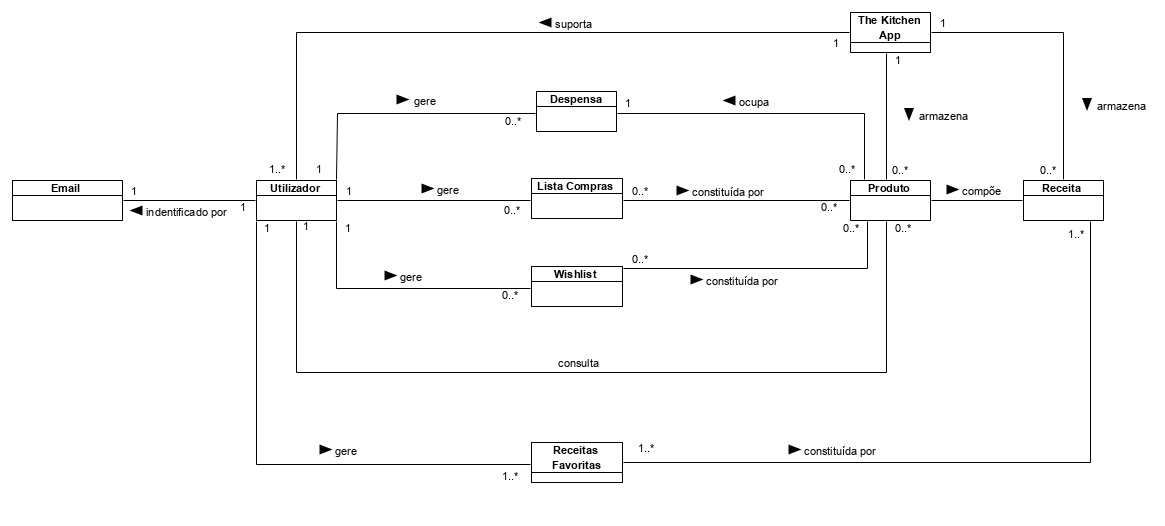
\includegraphics[width=\textwidth]{images/modelo_dominios.png}
        \caption{Modelo de Domínios}
\end{figure}

\chapter{Diagrama de Use Cases}
    \begin{figure}[H]
    \centering
        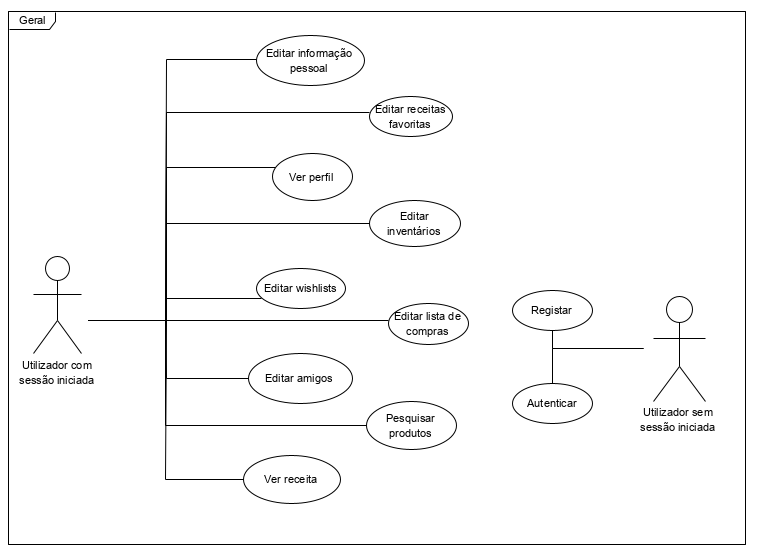
\includegraphics[width=\textwidth]{images/diagrama_use_cases.png}
    \end{figure}

\chapter{Especificação de Use Cases}
    \section{Registar}
        \begin{figure}[H]
        \centering
            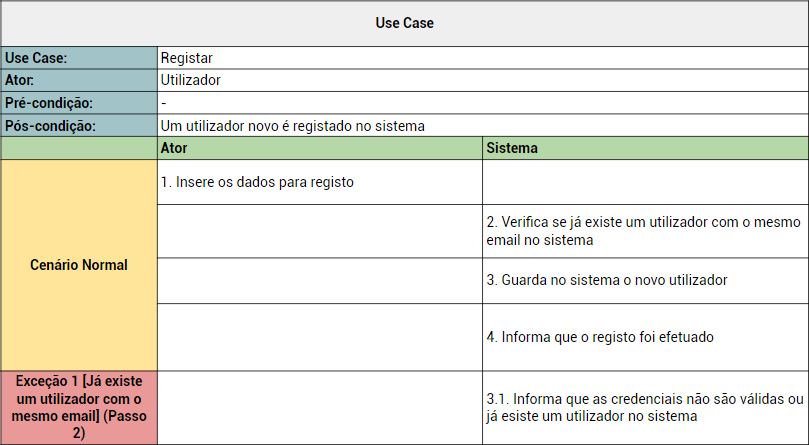
\includegraphics[width=\textwidth]{images/usecases/registar.png}
        \end{figure}

    \section{Autenticar}
        \begin{figure}[H]
        \centering
            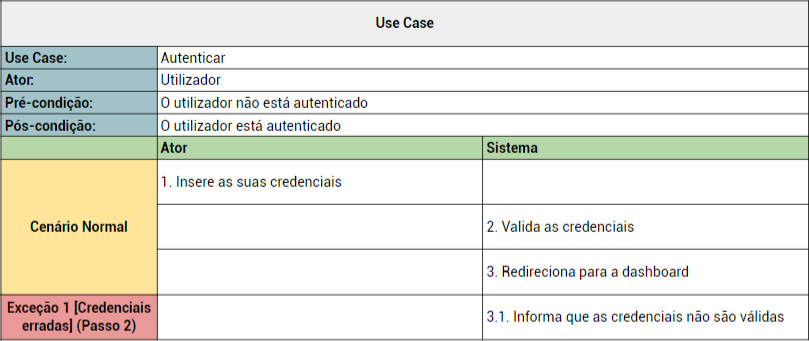
\includegraphics[width=\textwidth]{images/usecases/autenticar.png}
        \end{figure}

    \section{Editar informação pessoal}
        \begin{figure}[H]
        \centering
            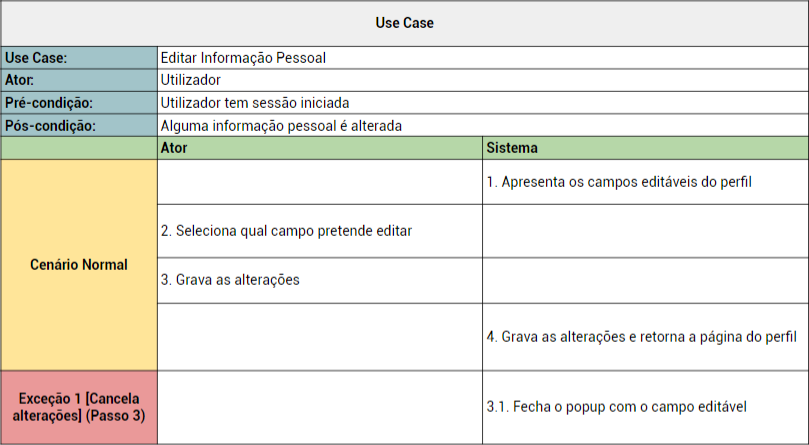
\includegraphics[width=\textwidth]{images/usecases/editar_utilizador.png}
        \end{figure}

    \section{Editar receitas favoritas}
        \begin{figure}[H]
        \centering
            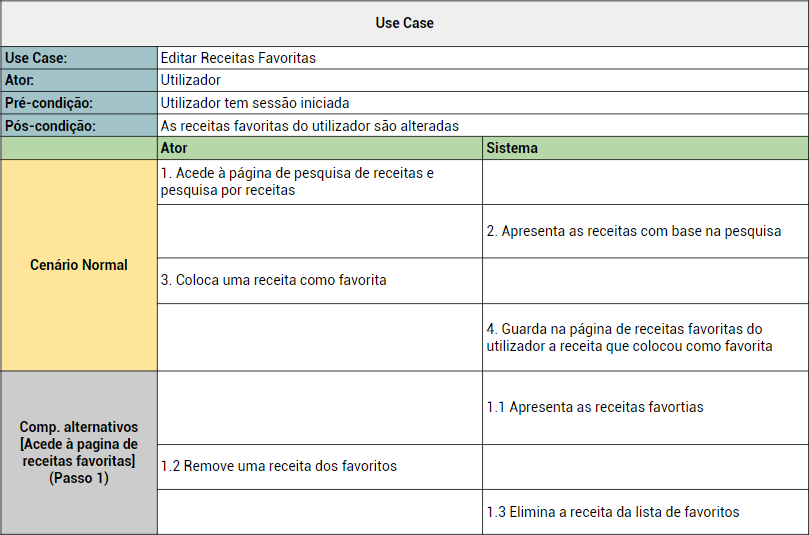
\includegraphics[width=\textwidth]{images/usecases/editar_receitas_favoritas.png}
        \end{figure}

    \section{Ver perfil}
        \begin{figure}[H]
        \centering
            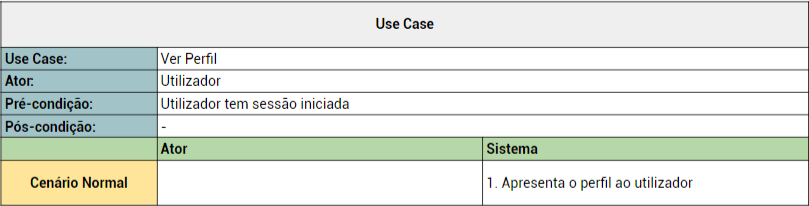
\includegraphics[width=\textwidth]{images/usecases/ver_perfil.png}
        \end{figure}

    \section{Editar inventários}
        \begin{figure}[H]
        \centering
            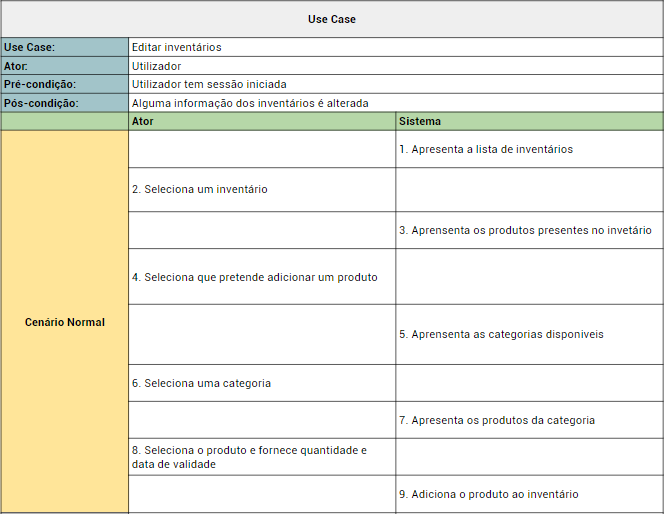
\includegraphics[width=\textwidth]{images/usecases/editar_iventarios_1.png}
            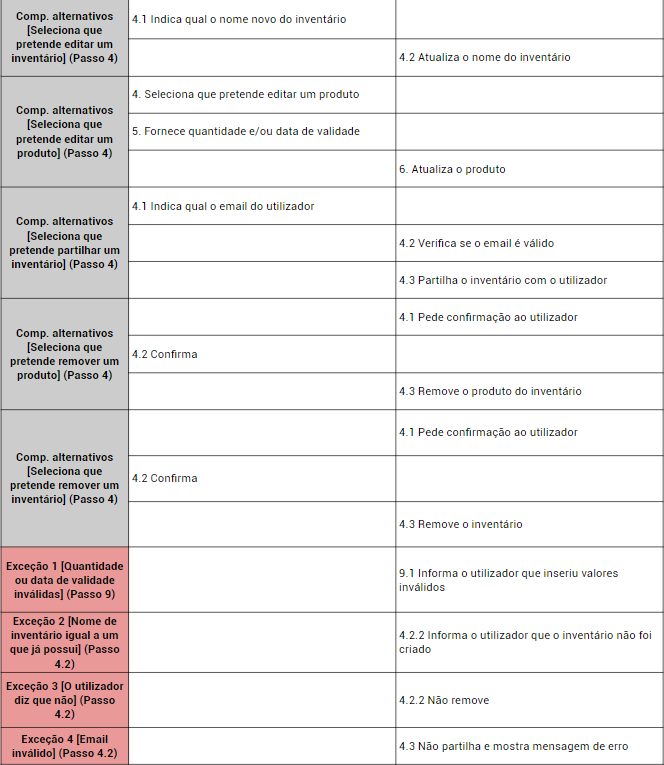
\includegraphics[width=\textwidth]{images/usecases/editar_iventarios_2.png}
        \end{figure}

    \section{Editar wishlists}
        \begin{figure}[H]
        \centering
            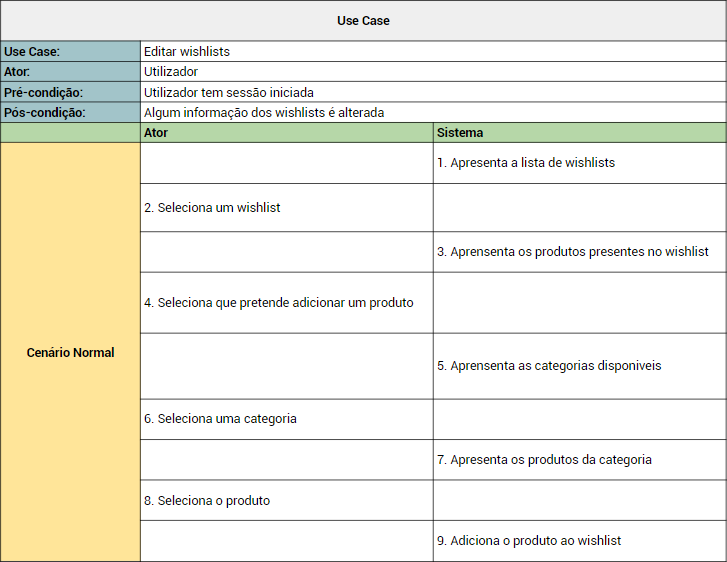
\includegraphics[width=\textwidth]{images/usecases/editar_whishlist_1.png}
            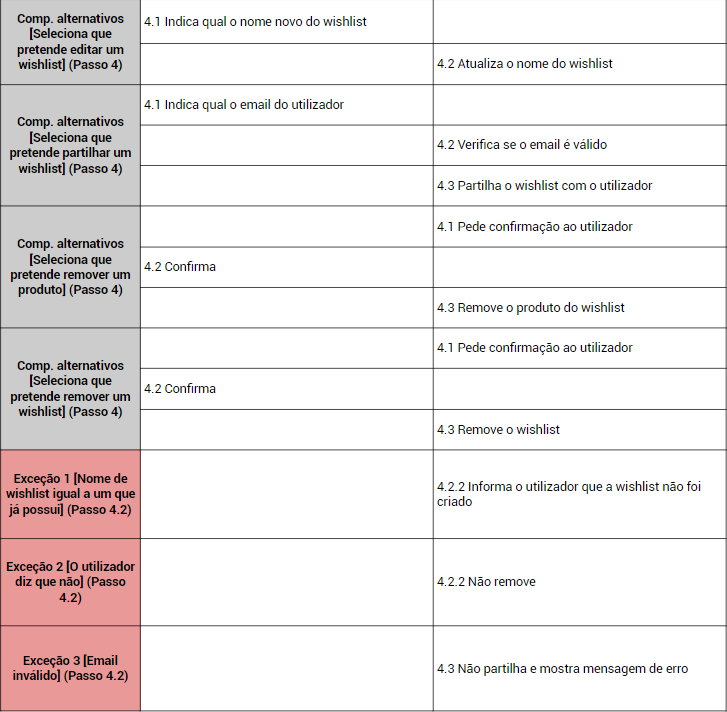
\includegraphics[width=\textwidth]{images/usecases/editar_whishlist_2.png}
        \end{figure}

    \section{Editar listas de compras}
        \begin{figure}[H]
        \centering
            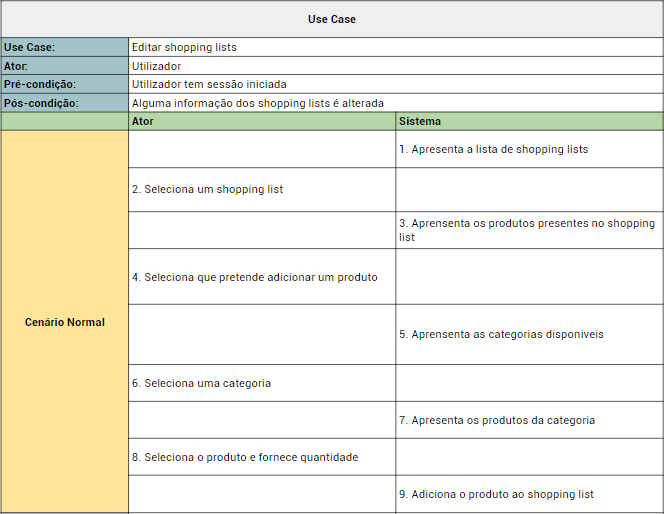
\includegraphics[width=\textwidth]{images/usecases/editar_shoppinglist_1.png}
            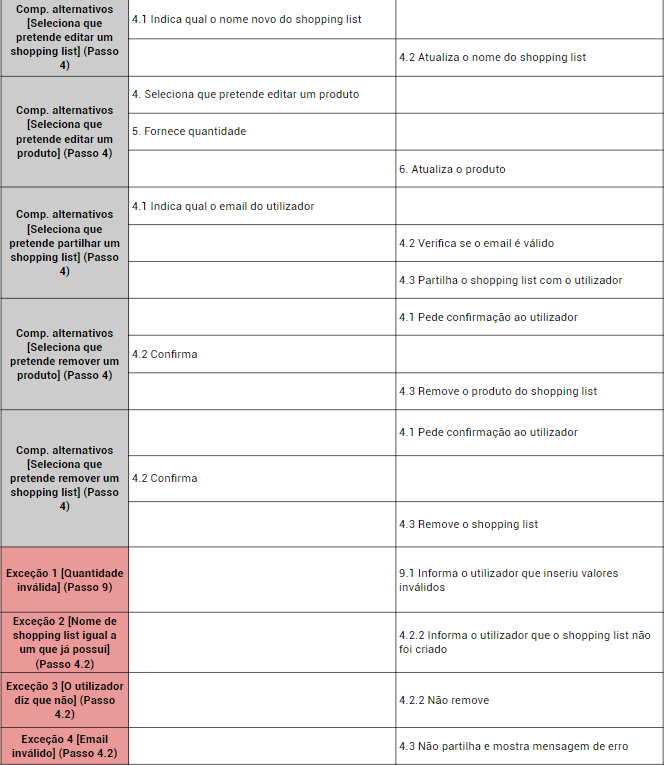
\includegraphics[width=\textwidth]{images/usecases/editar_shoppinglist_2.png}
        \end{figure}

    \section{Editar amigos}
        \begin{figure}[H]
        \centering
            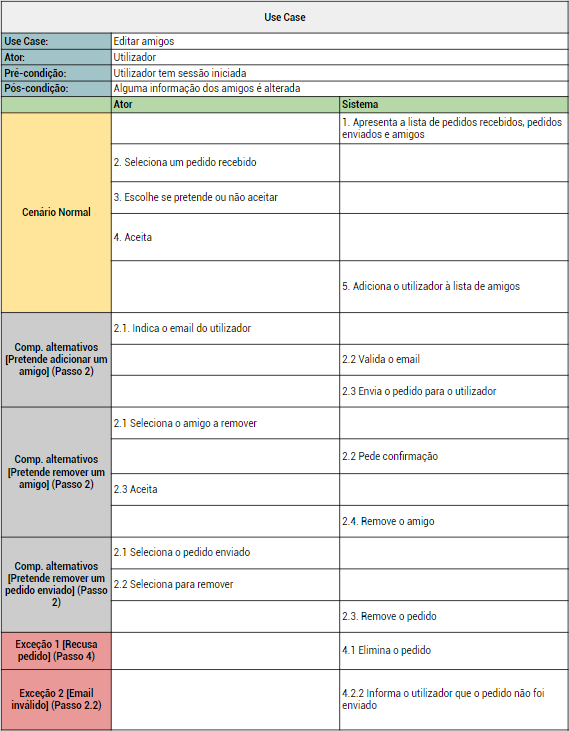
\includegraphics[width=\textwidth]{images/usecases/editar_amigos.png}
        \end{figure}

    \section{Pesquisar produtos}
        \begin{figure}[H]
        \centering
            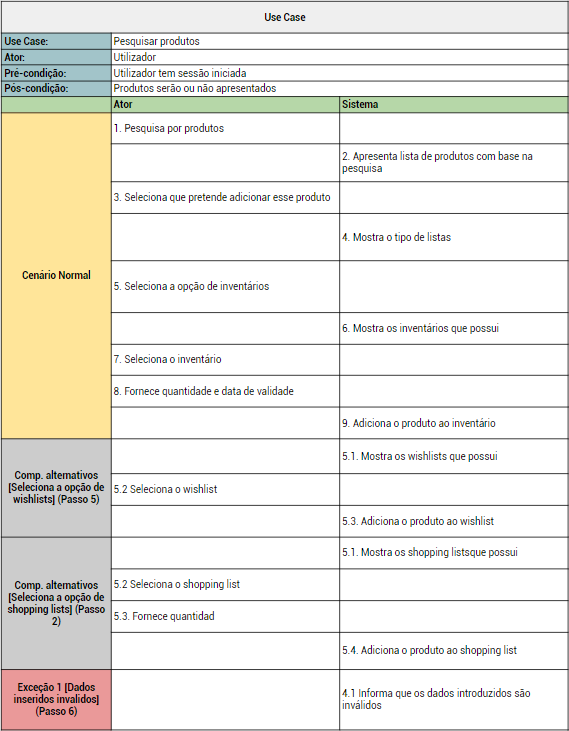
\includegraphics[width=\textwidth]{images/usecases/pesquisar_produto.png}
        \end{figure}

    \section{Ver receita}
        \begin{figure}[H]
        \centering
            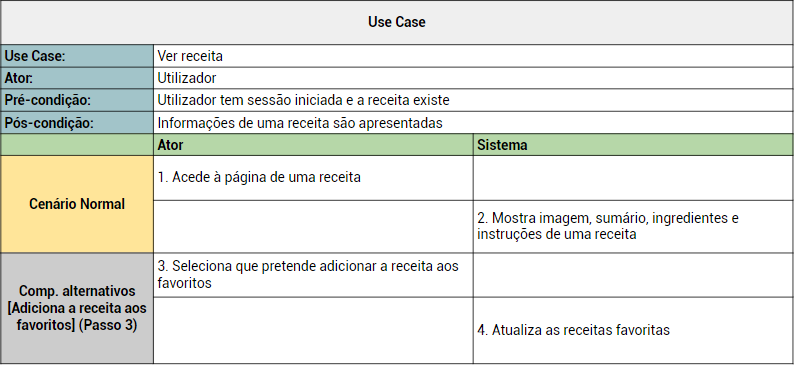
\includegraphics[width=\textwidth]{images/usecases/ver_receita.png}
        \end{figure}

\chapter{Arquitetura da Camada de Negócios}
    \section{Dicionário das Principais Classes}
        \subsection{User}
        Corresponde à representaão no sistema dos utilizadoeres registados,
        contendo a sua informação pessoal e credenciais de acesso.
        \subsection{Product}
        Representa a unidade básica de todas as dispensas, listas de compras e
        listas de favoritos. Contém informação do nome, categoria, preço e
        quantidades por embalagem. Existem classes referentes aos vários tipos
        de produtos, que herdam desta, e contêm informação extra para ser
        possível acomodar os diferentes tipos de listas presentes no programa.
        \subsection{Inventory}
        A classe Inventory representa uma lista de produtos de um utilizador, contendo
        informação sobre o seu dono, nome e produtos disponíveis nesta, e 
        com quem é partilhada. A lista de produtos tem que pertencer à super
        classe \textit{Product}, e vai ser isto que vai determinar a que
        corresponde o inventário em questão, se é uma dispensa, lista de
        favoritos ou de compras.
        \subsection{Recipe}
        Esta classe representa uma receita, contendo informação sobre o seu
        nome, resumo, ingredientes necessários à confeção e instruções de
        preparação.
    \section{Descrição da Arquitetura}
    Cada utilizador possui uma lista de dispensas, uma lista de listas de 
    produtos favoritos, uma lista de listas de compras e uma lista de receitas
    favoritas.
    Também existe a possibilidade de um utilizador partilhar as suas listas de
    produtos, tendo cada utilizador uma lista de inventários partilhados
    consigo.
    \section{Diagrama de Classes}
        \begin{figure}[H]
        \centering
                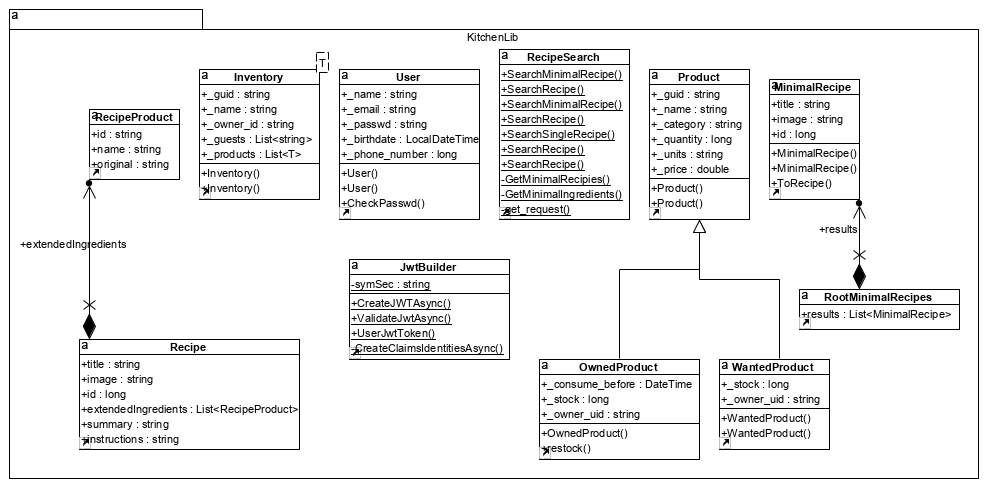
\includegraphics[width=\textwidth]{images/diagrama_de_classes.png}
        \end{figure}

    \section{Diagrama de ORM}
        \begin{figure}[H]
        \centering
            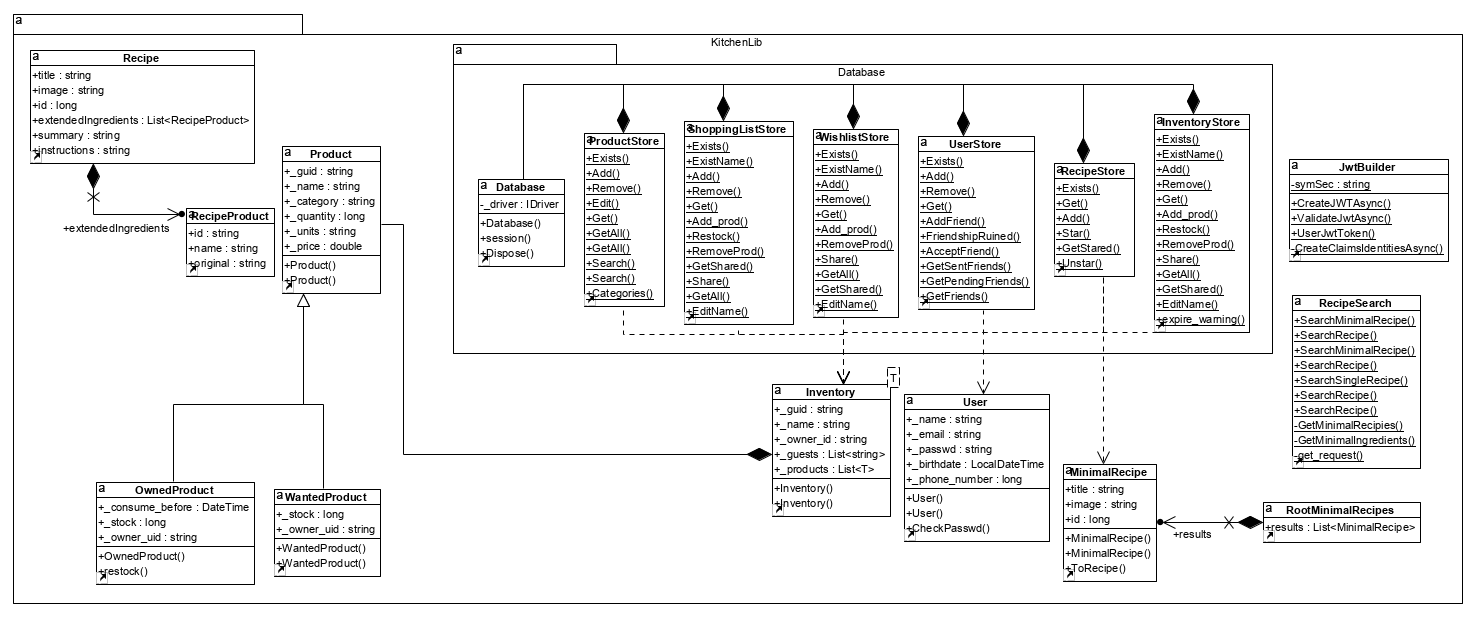
\includegraphics[width=\textwidth]{images/diagrama_de_ORN.png}
        \end{figure}

\chapter{Proposta de Interface}
    \begin{figure}[H]
    \centering
            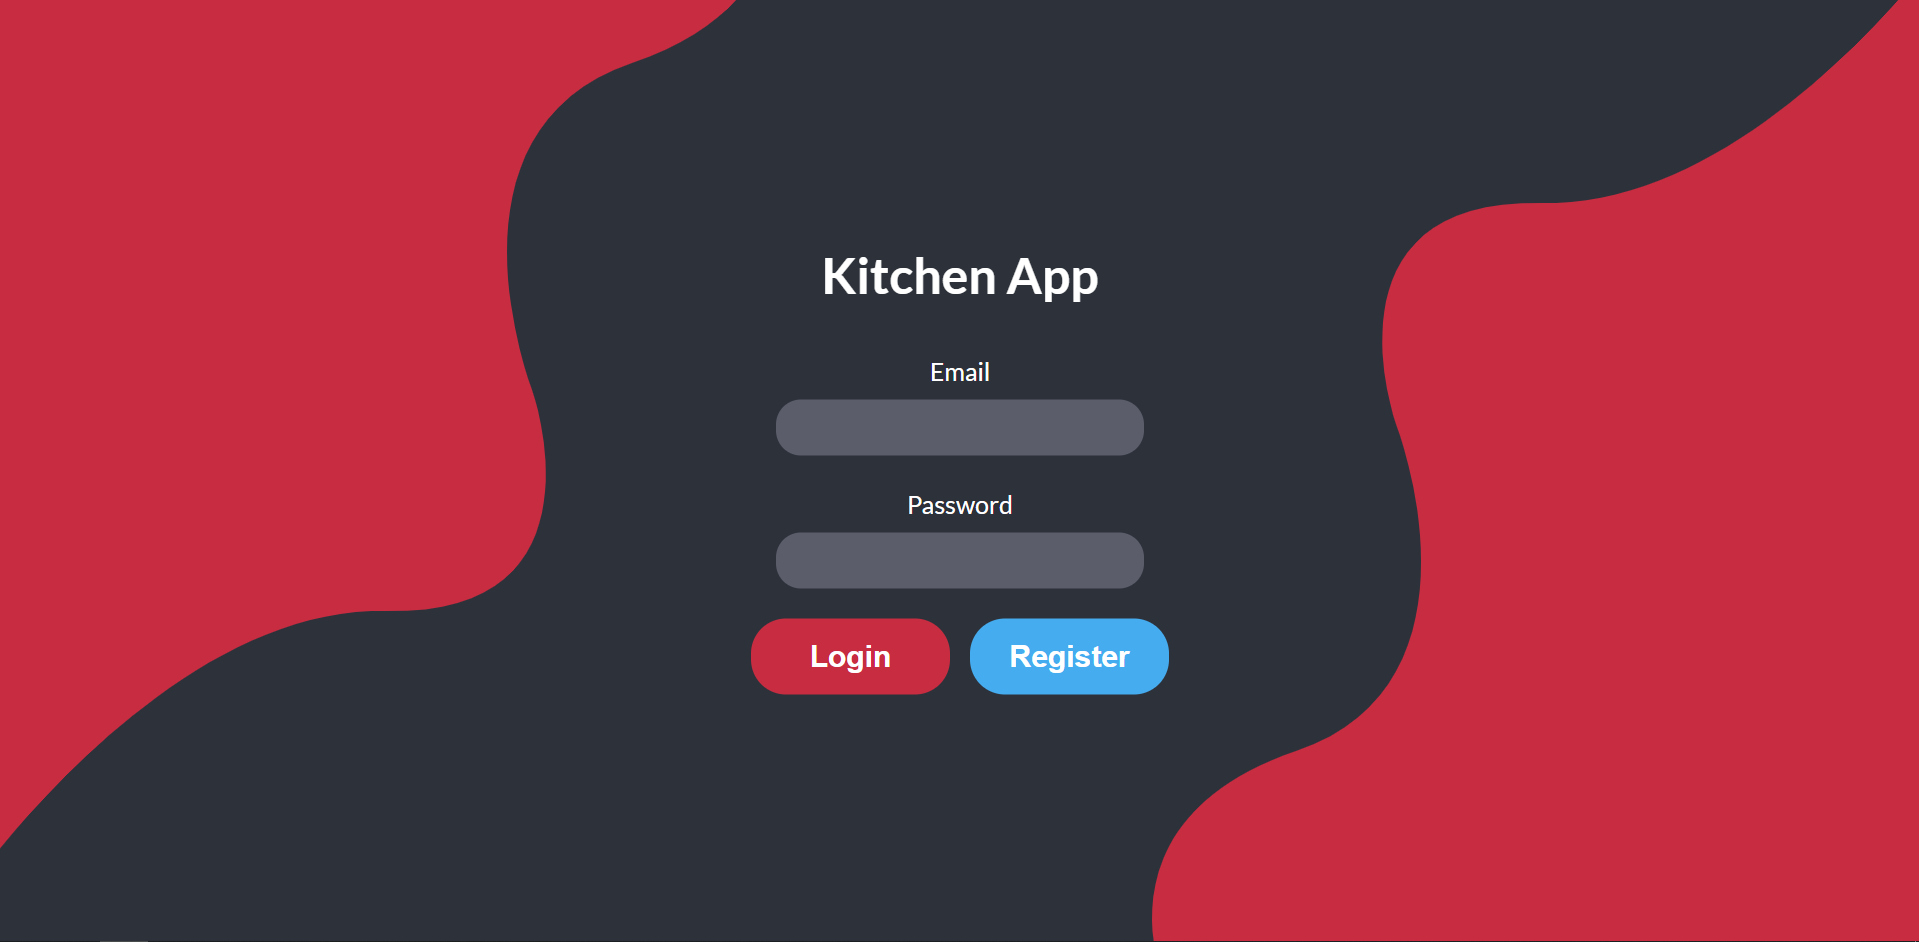
\includegraphics[width=0.9\textwidth]{images/mockup/login_desktop.png}
            \caption{Login no Desktop}
    \end{figure}
    \begin{figure}[H]
    \centering
            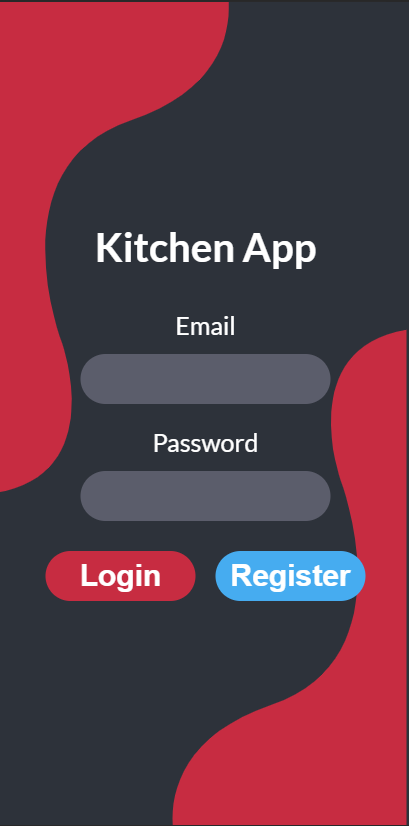
\includegraphics[width=0.4\textwidth]{images/mockup/login_mobile.png}
            \caption{Login em Mobile}
    \end{figure}
    \begin{figure}[H]
    \centering
            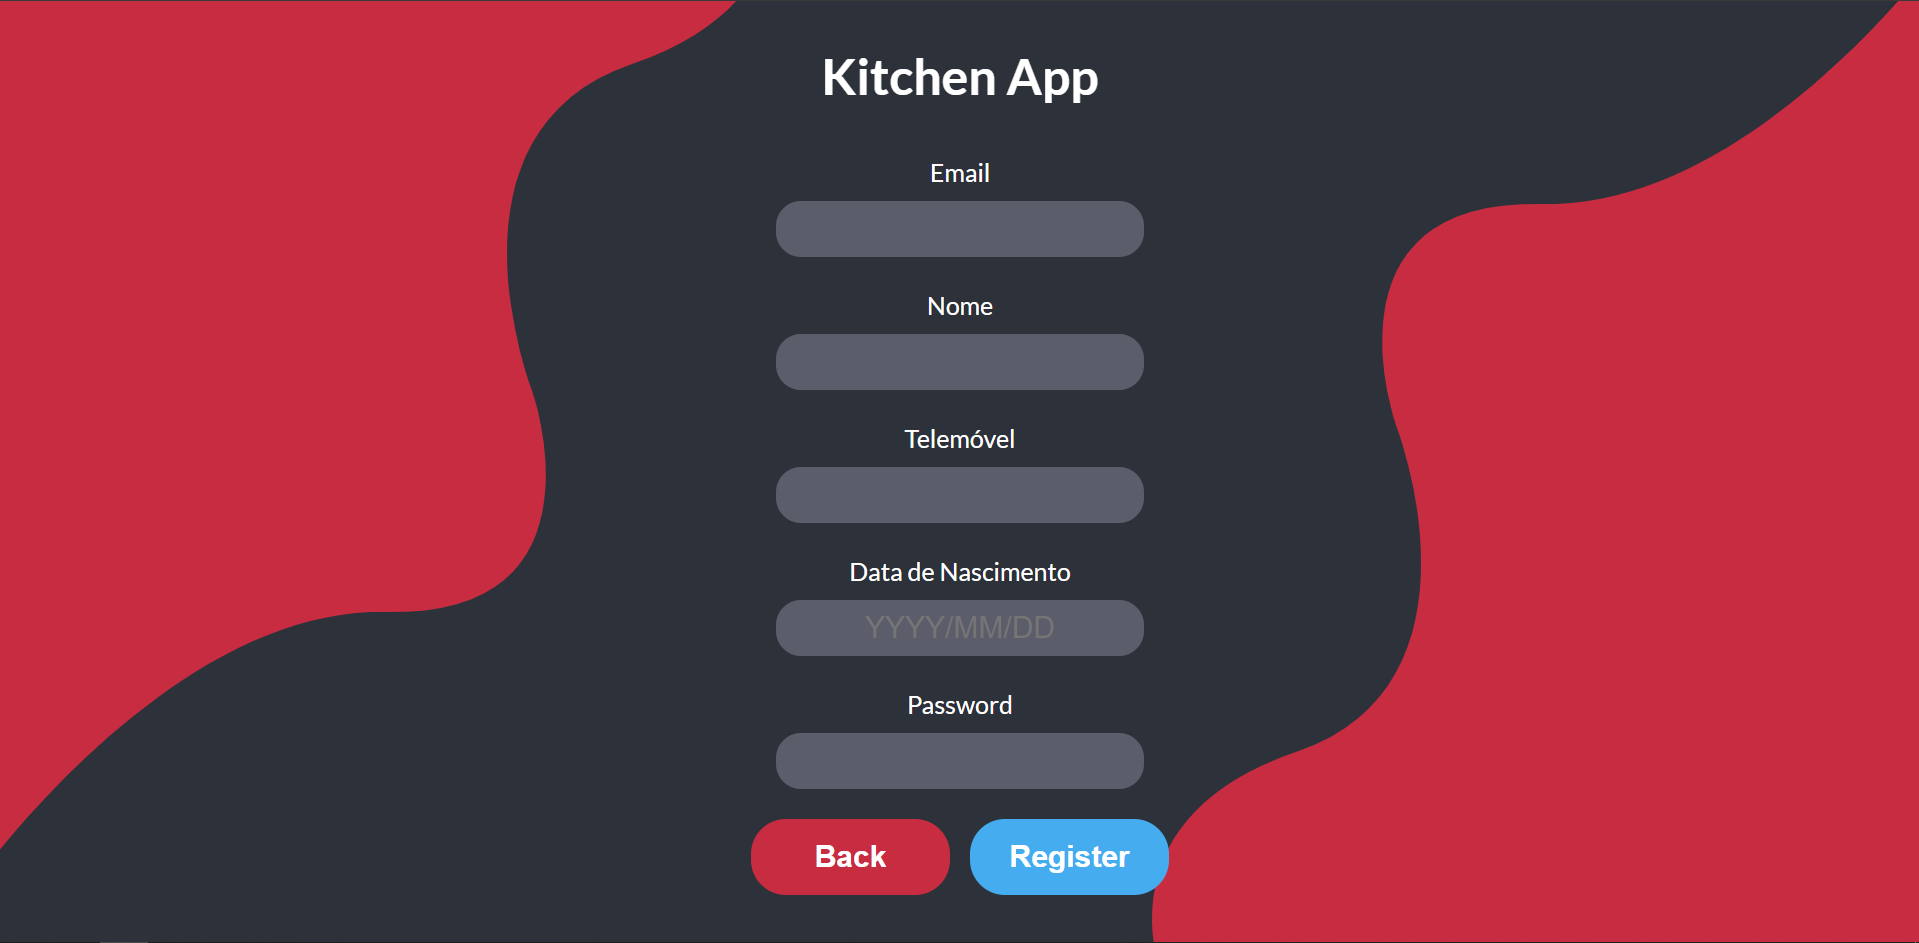
\includegraphics[width=0.9\textwidth]{images/mockup/register_desktop.png}
            \caption{Registo no Desktop}
    \end{figure}
    \begin{figure}[H]
    \centering
            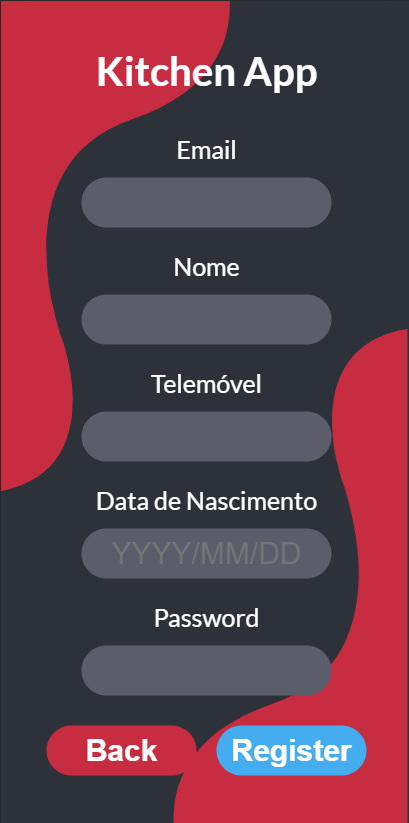
\includegraphics[width=0.4\textwidth]{images/mockup/register_mobile.png}
            \caption{Registo em Mobile}
    \end{figure}
    \begin{figure}[H]
    \centering
            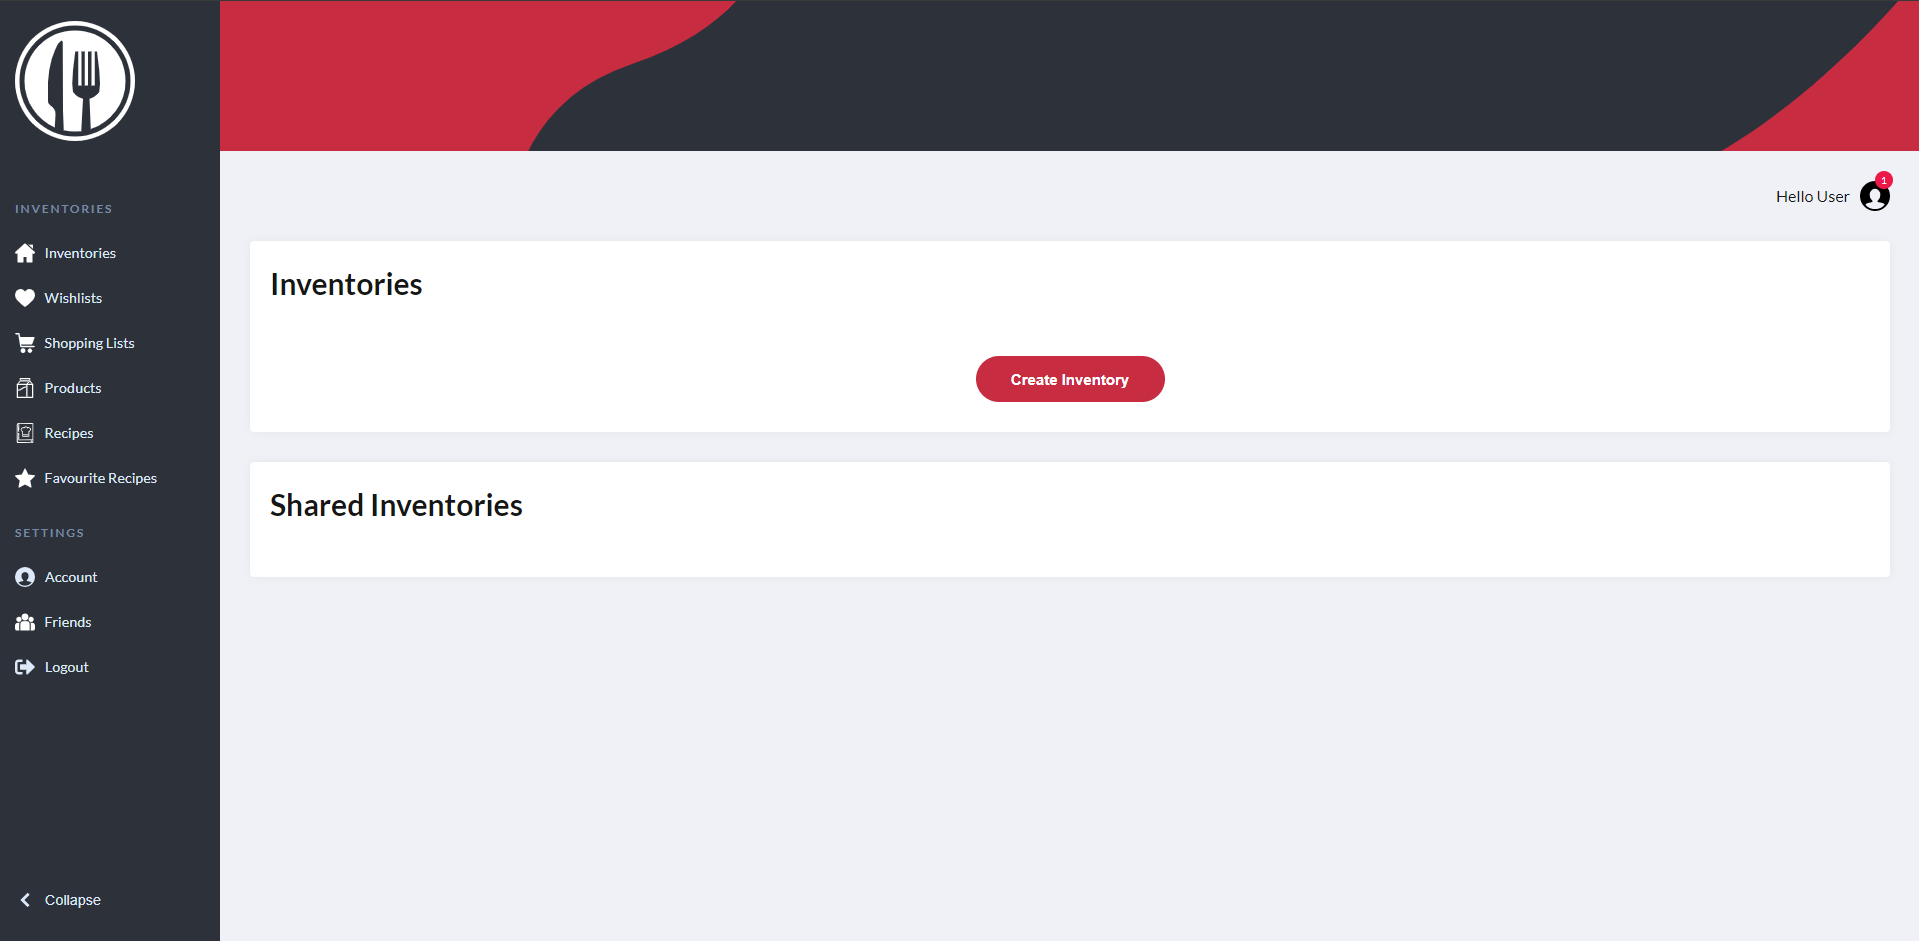
\includegraphics[width=0.9\textwidth]{images/mockup/dashboard_desktop.png}
            \caption{Dashboard no Desktop}
    \end{figure}
    \begin{figure}[H]
    \centering
            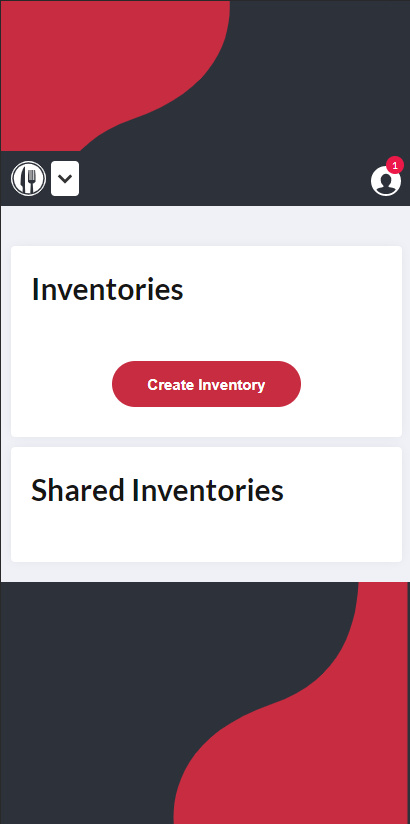
\includegraphics[width=0.4\textwidth]{images/mockup/dashboard_mobile.png}
            \caption{Dashboard em Mobile}
    \end{figure}
    

\chapter{Metodologia de Implementação}
O padrão arquitetural escolhido para a implementação da aplicação foi o MVC
(\textit{Model View Controller}), por forma a obter um conjunto de pequenos
componentes modulares de fácil integração, e assim facilitar o desenvolvimento 
em paralelo. De forma a tornar a implementação ainda mais modular, a componente
do controlador foi decomposta em pequenos controladores individuais, cada um
responsável por lidar com uma pequena parte da aplicação, como por exemplo,
lidar com as dispensas, ou com a autenticação.

A escolha deste padrão arquitetural proporciona também uma camada de abstação,
deixando a possibilidade de implementar a aplicação em mais do que uma
plataforma, sem fazer alterações ao préviamente feito.

A componente do modelo foi decomposta em camada de negócio e de dados, por forma
a garantir a consitência, integridade e disponibilidade dos dados da aplicação,
qualquer que seja a tecnologia utilizada para o suporte da base de dados.

\chapter{Ferramentas utilizadas na implementação}

A principal ferramenta utilizada para a implementação da aplicação apresentada
foi a \textit{framework} de desenvolvimento ASP.NET Core. Esta escolha foi
tomada graças à excelente documentação disponível e simplicidade de utilização.

Como gestor de base de dados escolhemos o \textit{Neo4j}, que utiliza um modelo
não relacional e que se enquadra com a disposição definida dos dados da
aplicação.

Para a criação da interface do produto final, foi utilizada a biblioteca
\textit{React}, assente na linguagem de programação \textit{JavaScript}, pela
sua popularidade e facilidade de utilização.

Para tornar o \textit{deployment} da aplicação o mais agnóstico da máquina onde
é feito, e para facilitar os testes feitos durante o processo de
desenvolvimento, foi utilizada a ferramenta \textit{Docker} e \textit{Docker
Compose}, na qual foram criados \textit{containers} contendo a aplicação, todas
as suas configurações, tornando o processo de correr a aplicação apenas um
comando, sem haver qualquer preocupação ao nível de \textit{networking}.

De forma a validar os pedidos chegados à aplicação, e encaminha-los para o
devido controlador, utilizamos como \textit{Reverse Proxy} a ferramenta
\textit{Nginx}.

Para garantir a disponibilidade da aplicação a qualquer hora, esta foi hospedada
na plataforma \textit{Azure}, tirando partido do esforço anterior de utilização
da ferramenta \textit{Docker}.

Por fim, foram utilizados diversos \textit{browsers}, como o \textit{Firefox} ou
o \textit{Brave}, em várias plataformas, para garantir a boa aparência da
interface apresentada ao utilizador final.

\chapter{Desenvolvimento do Projeto}
    \section{Conexão da Base de Dados}
    Após a instalação e configuração do motor de base de dados Neo4j, passamos à
    integração deste com a aplicação em desenvolvimento. Para o processo de
    conexão entre ambas as partes utilizamos o \textit{Neo4jDotNetDriver},
    pacote oficial deste motor de base de dados para a linguagem de programação
    em uso, \textit{C\#}.

    Como o Neo4j dispensa uma geração incial da base de dados, partimos para a
    escrita de queries que manipulasse esta, de forma a que, quando esta estiver
    povoada, se assemelhe ao inicialmente proposto.

    Para povoar a base de dados, optamos por apenas introduzir produtos, sendo
    contas de utilizadores criadas à medida que necessário.

    \section{Pesquisa e Sugestão de Receitas}
    Para complementar a funcionalidade chave desta aplicação, gestão de stocks
    de despensas, foi integrado na aplicação uma API externa, chamada
    \textit{Spoonacular}, capaz de fornecer receitas culinárias, permitindo uma
    pesquisa bastante detalhada sobre estas.

    Assim, implementamos na aplicação a capacidade de pesquisa de receitas por
    nome, e a capacidade de sugerir receitas com base no que existe numa
    despensa.

    \section{Gestão de Logins}
    Por forma a simplificar a gestão do utilizador que faz os pedidos,
    implementamos um sistema de tokens, assente no standard \textit{JSON Web
    Token} (\textit{JWT}), que contém informação sobre o utilizador, prazo de
    validade e também uma assinatura digital que marca a autenticidade do mesmo,
    não dando assim acessos indevidos às páginas privadas do utilizador. Este
    token é validado e renovado a cada pedido efetuado, e é transmitido num
    header do pedido \textit{HTTP}.

\chapter{Arquitetura Final do Projeto}
Após a implementação da aplicação, a arquitetura final tem o seguinte aspeto:
\begin{figure}[H]
    \centering
        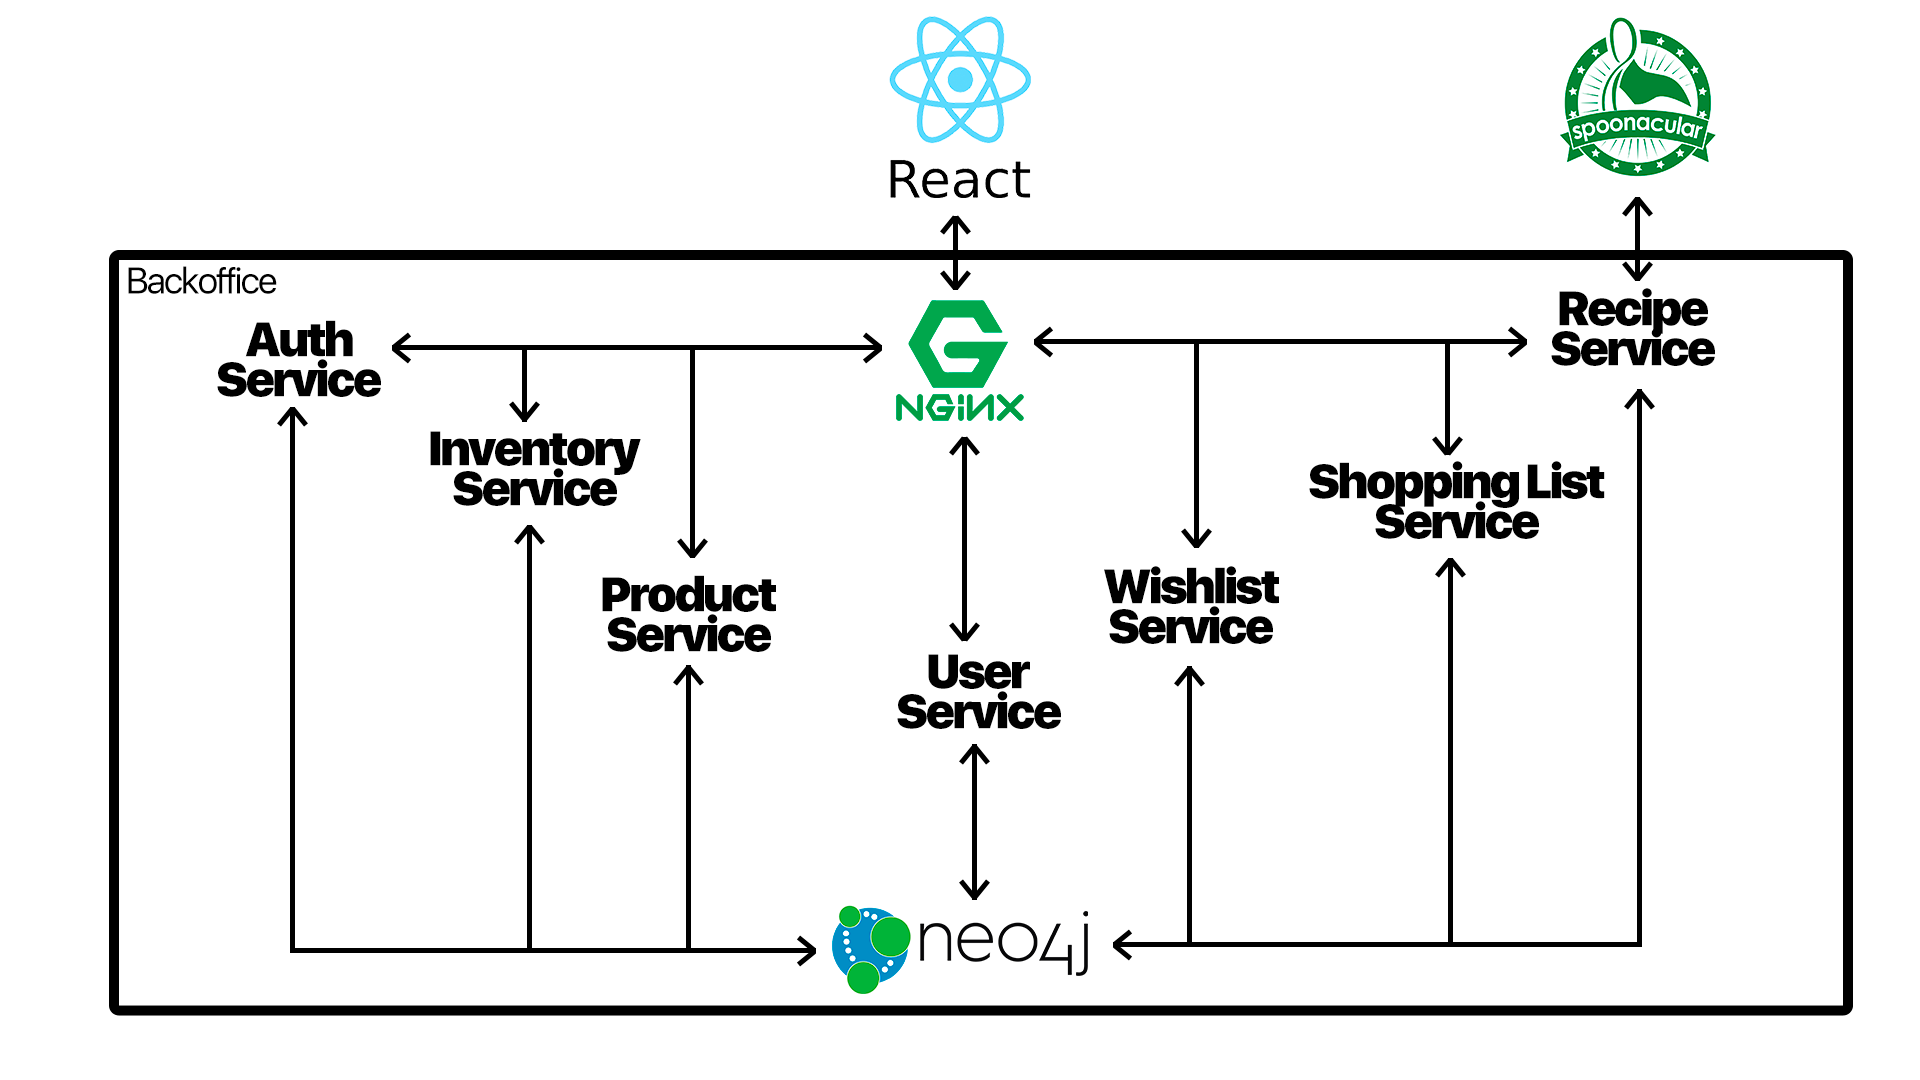
\includegraphics[width=\textwidth]{images/arquitetura.png}
        \caption{Arquitetura Final da Aplicação}
\end{figure}

No backoffice, os pedidos são efetuados pela \textit{Web API} definida e
documentada, e são atendidos pelo \textit{nginx}, e posteriormente 
encaminhados para o serviço referente ao pedido recebido. Caso sejam 
pedidos que necessitem autenticação, antes de encaminhados para o serviço 
correto, ainda passam pelo \textit{Auth Service}, responsável pela autenticação 
dos utilizadores. Apenas é exposta a ligação ao \textit{proxy} ao exterior,
sendo todas as restantes conexões aos serviços e base de dados feitas
internamente. Apenas um dos serviços faz conexões diretas ao exterior, sendo
este o referente às receitas, que faz pedidos à API externa integrada.

O frontend comunica com os backend com os mesmos métodos acima descritos,
sendo o backend completamente independente do frontend.

\chapter{Produto Final}

    Ao longo de várias semanas a nossa equipa desenvolveu o Kitchen App até que
    o produto de software final fosse o inicialmente idealizado. Abaixo, iremos
    demonstrar como a aplicação funciona no geral e onde se encontra e como
    estão implementadas as nossas funcionalidades.

    \section{Página inicial (Sem sessão iniciada)}
    A página de login é a inicial e principal quando não se está 
    autenticado. Redirecionados para esta página são os utilizadores que
    ou não se autenticaram ou então não possuem um token válido (exemplos destes 
    são os utilizadores que se encontram autenticados na aplicação há tempo
    suficiente para que o seu token perdesse a validade). Nesta página é 
    então possível um utilizador autenticar se ou aceder à página de registo.

    \begin{figure}[H]
        \centering
            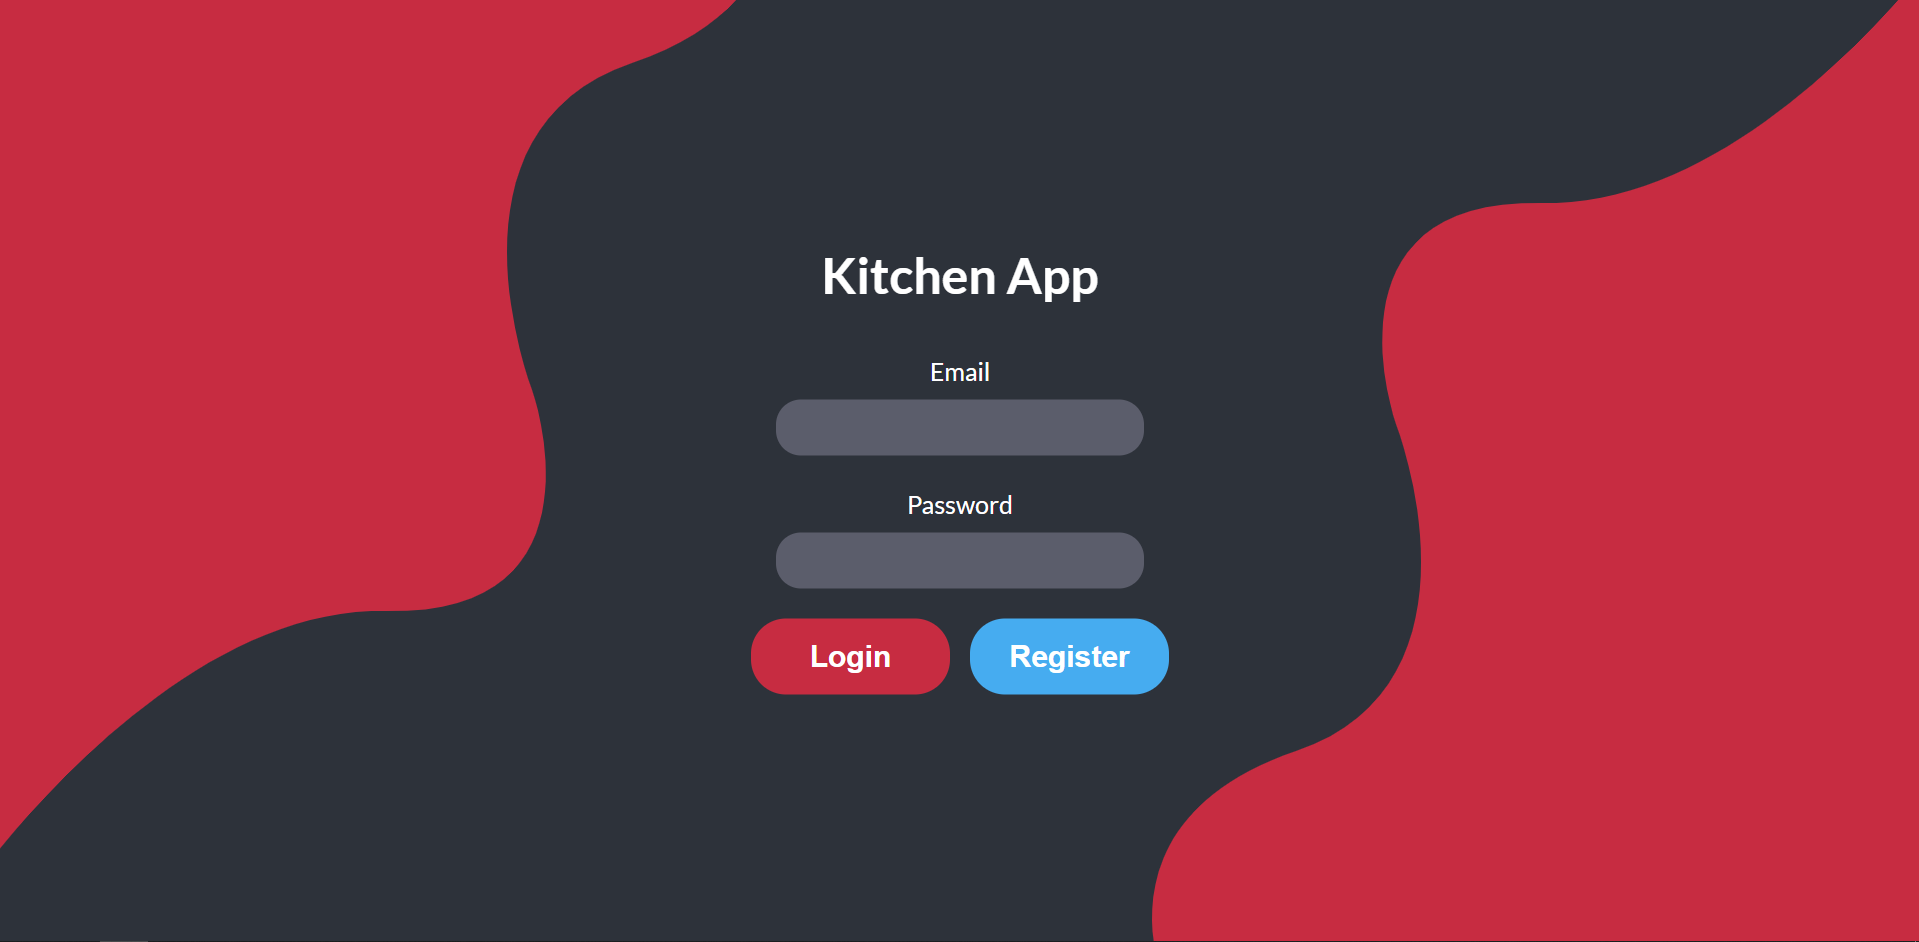
\includegraphics[width=\textwidth]{images/produto_final/login.png}
    \end{figure}

    Através então \textbf{da opção de Registo} é se direcionado para esta 
    página onde se é possível realizar o registo de um utilizador. Caso 
    não se pretenda realizar um registo podemos voltar para a página de login
    na opção \textbf{back}.

    \begin{figure}[H]
        \centering
            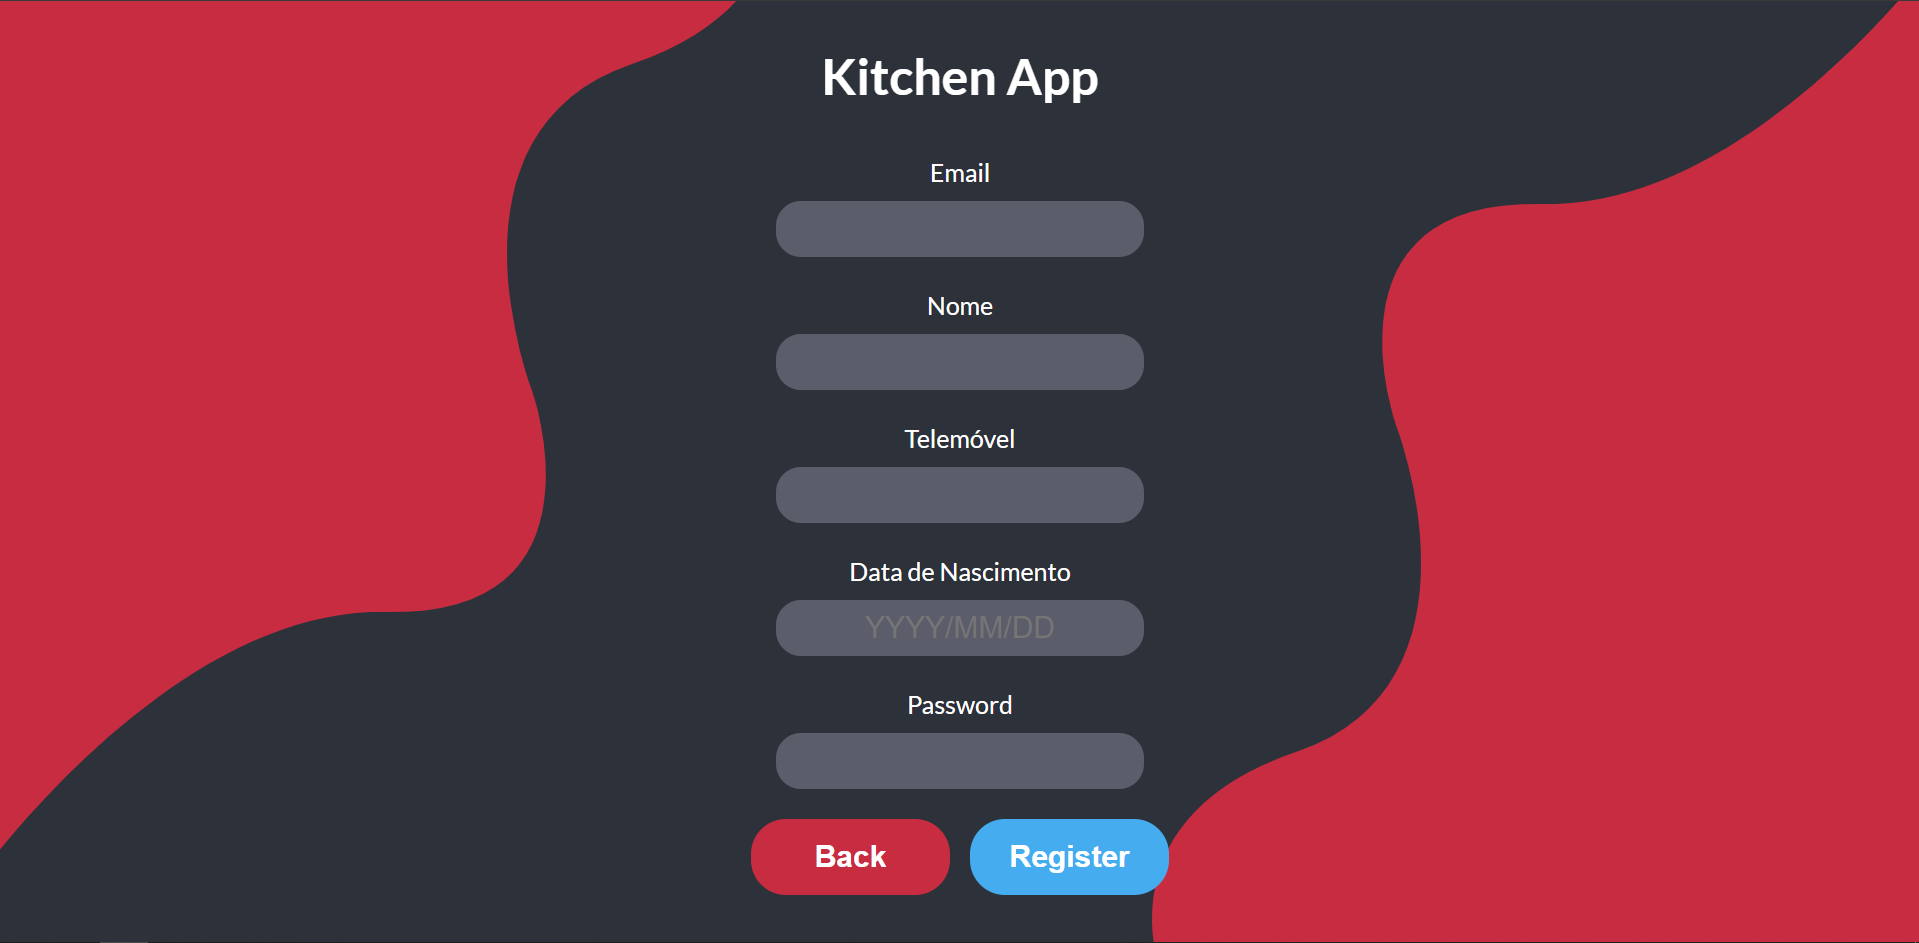
\includegraphics[width=\textwidth]{images/produto_final/registo.png}
    \end{figure}

    \section{Página inicial (com sessão iniciada)}

    Estando autenticado, é apresentado ao utilizador a sua \textbf{dashboard}.
    Nesta é possivel ver todos os \textbf{inventários} que o utilizador possui
    (próprios e partilhados), as \textbf{notificações} (serão mostradas mais 
    tarde) e todas as opções no \textbf{menu da esquerda} para nos ser 
    possível mover na aplicação (tanto as notificações como o menu lateral 
    esquerdo estão presentes em todas as páginas que é necessário 
    autenticação).

    \begin{figure}[H]
        \centering
            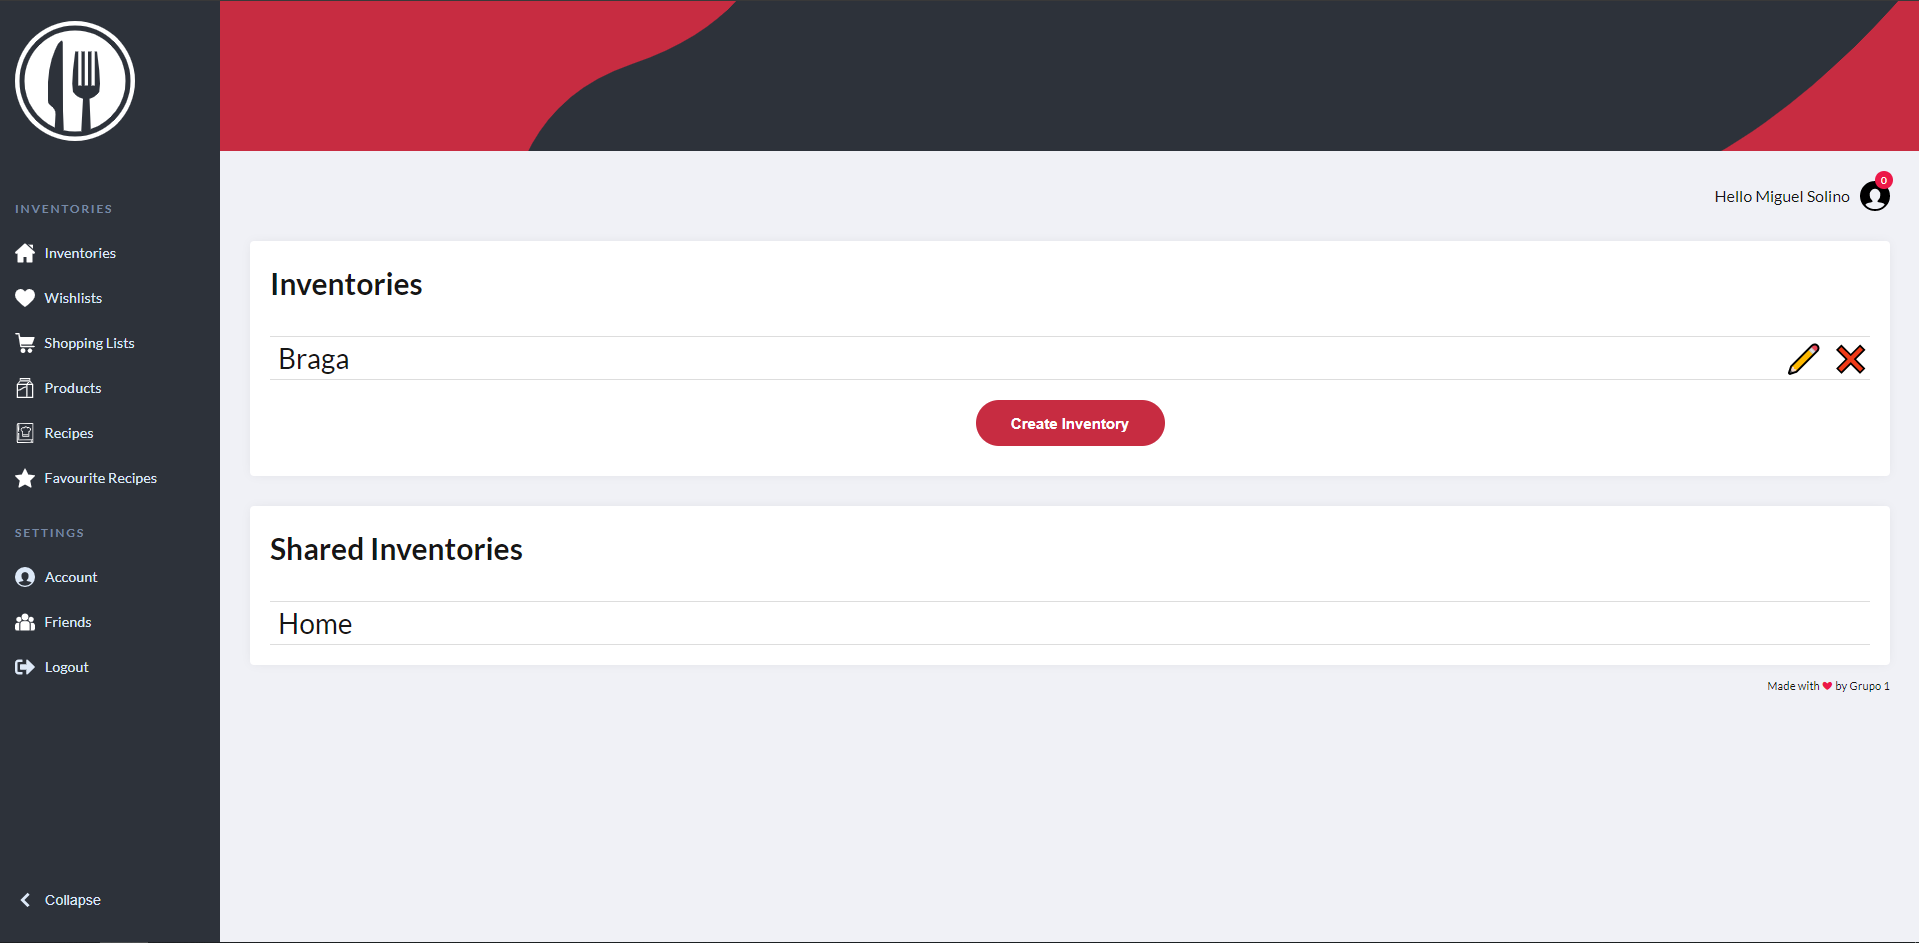
\includegraphics[width=\textwidth]{images/produto_final/inicial.png}
    \end{figure}

    \section{Inventário}

    Selecionando um inventário na página inicial é nos apresentada a página
    abaixo com todos os produtos que possui e as opções necessárias para 
    ser possível gerir o inventário e os produtos presentes. Nas figuras
    abaixo conseguimos ver o workflow de como se utiliza cada funcionalidade
    de um inventário.

    \begin{figure}[H]
        \centering
            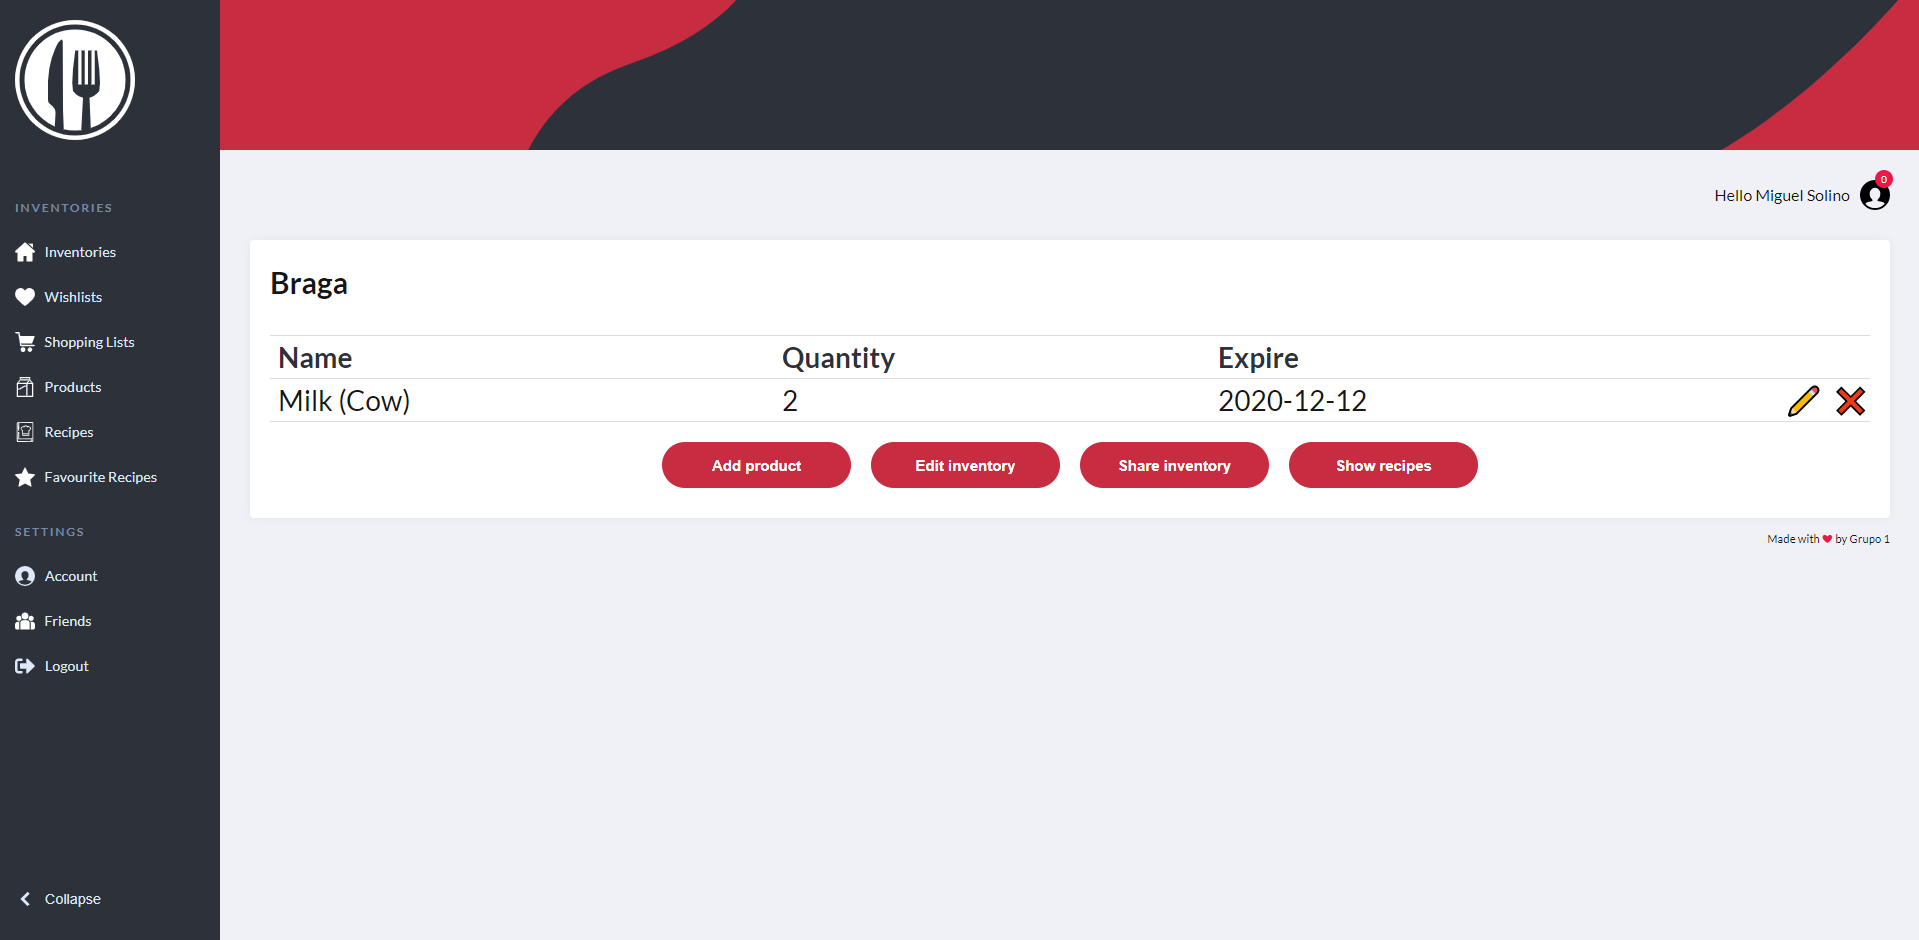
\includegraphics[width=\textwidth]{images/produto_final/iventario.png}
    \end{figure}

    \begin{figure}[H]
        \centering
            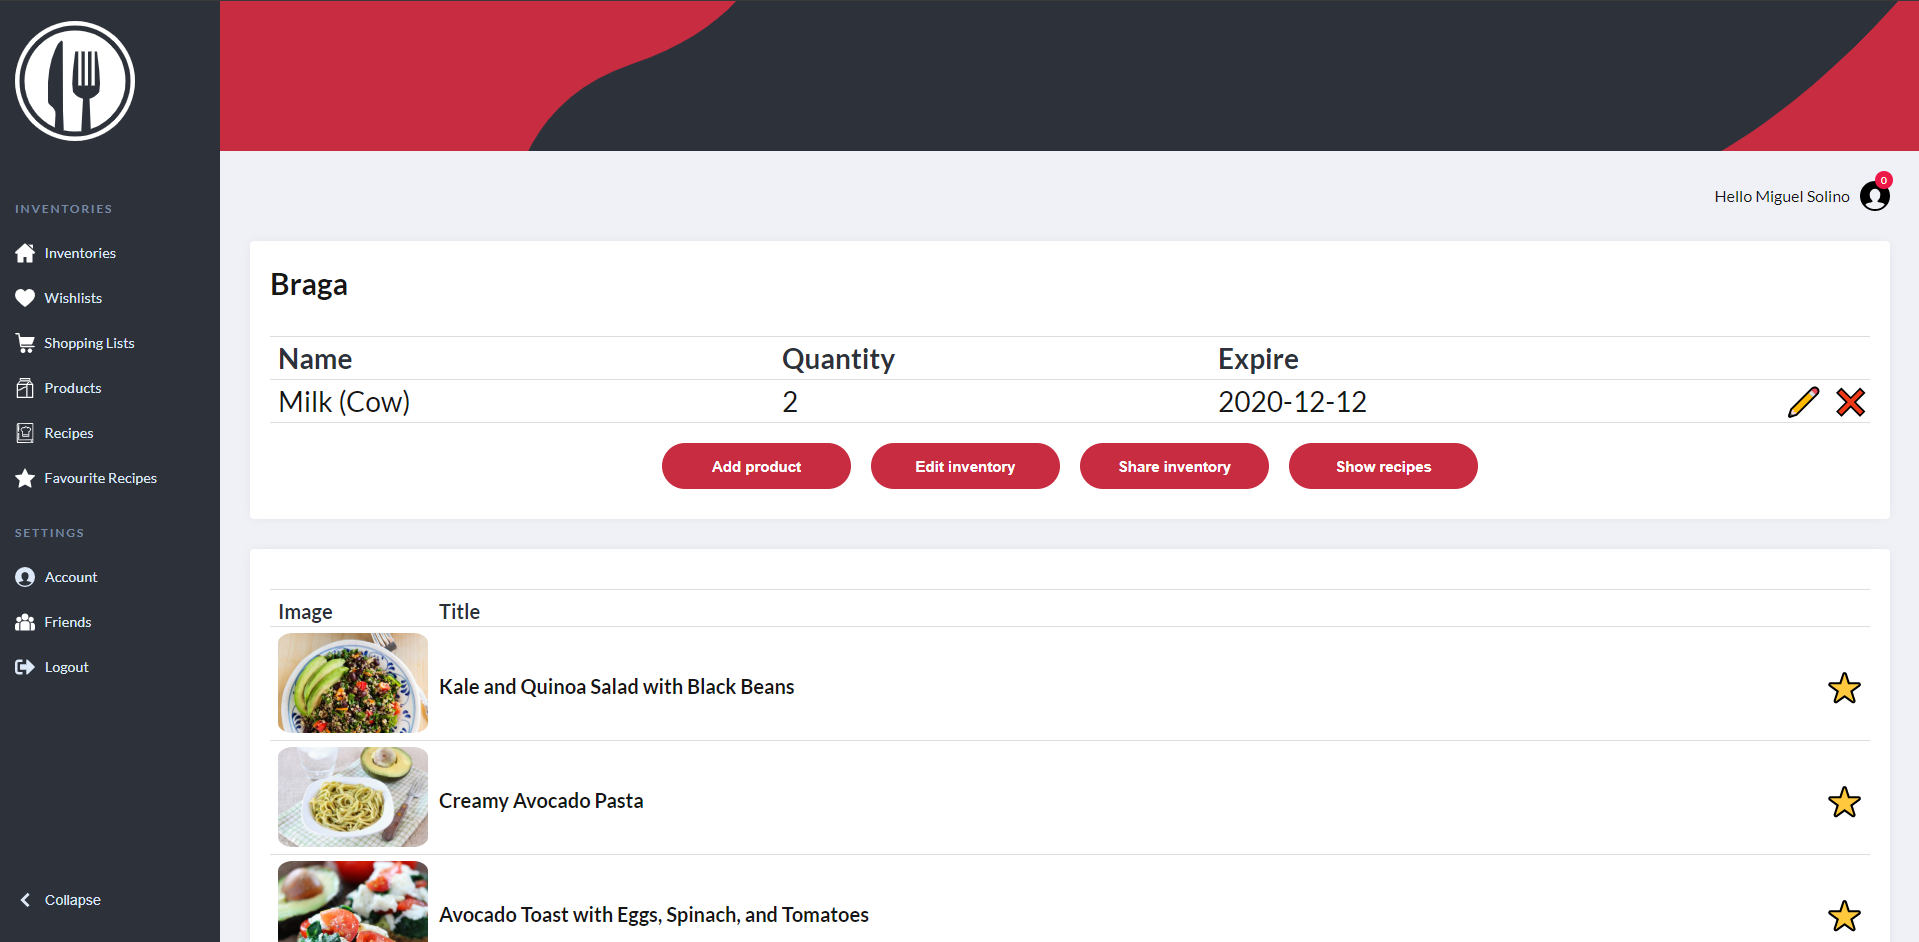
\includegraphics[width=\textwidth]{images/produto_final/iventario_receitas.png}
    \end{figure}

    \begin{figure}[H]
        \centering
            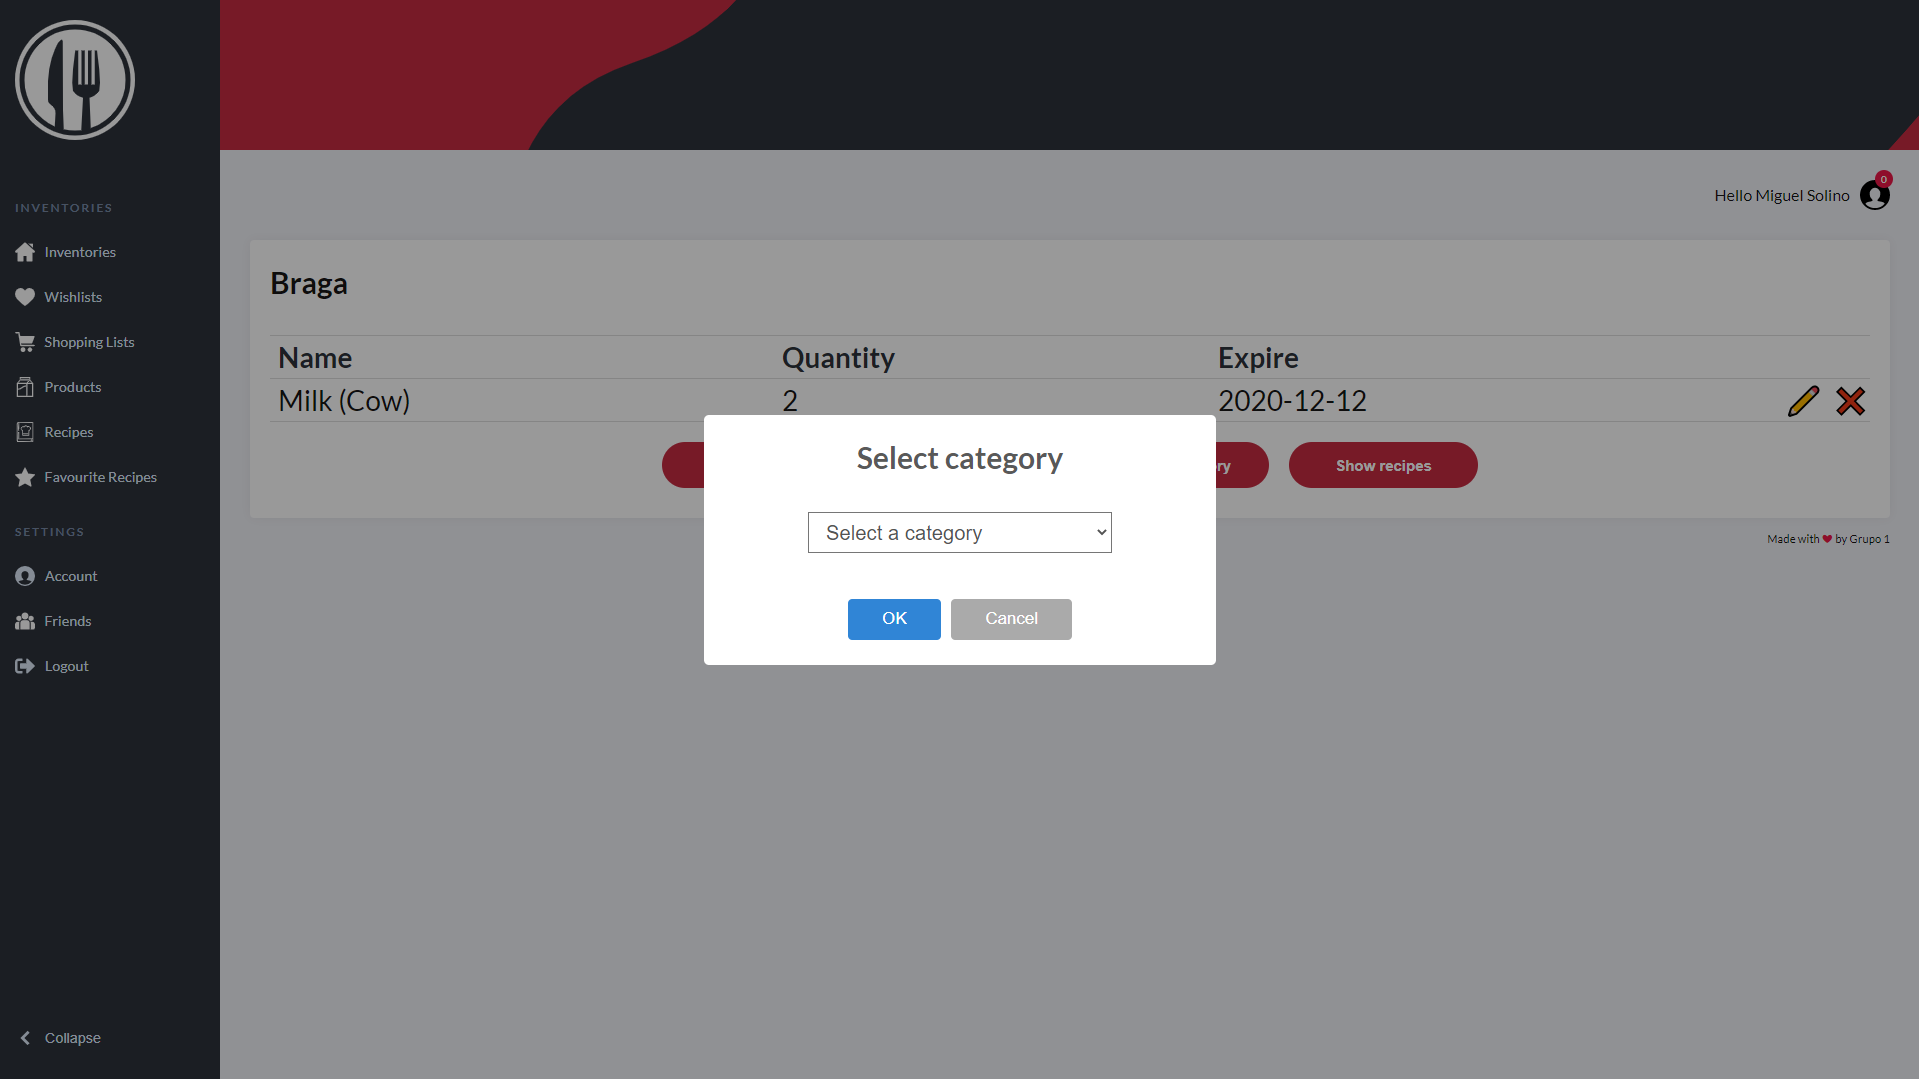
\includegraphics[width=\textwidth]{images/produto_final/inserir_produto_categoria.png}
    \end{figure}

    \begin{figure}[H]
        \centering
            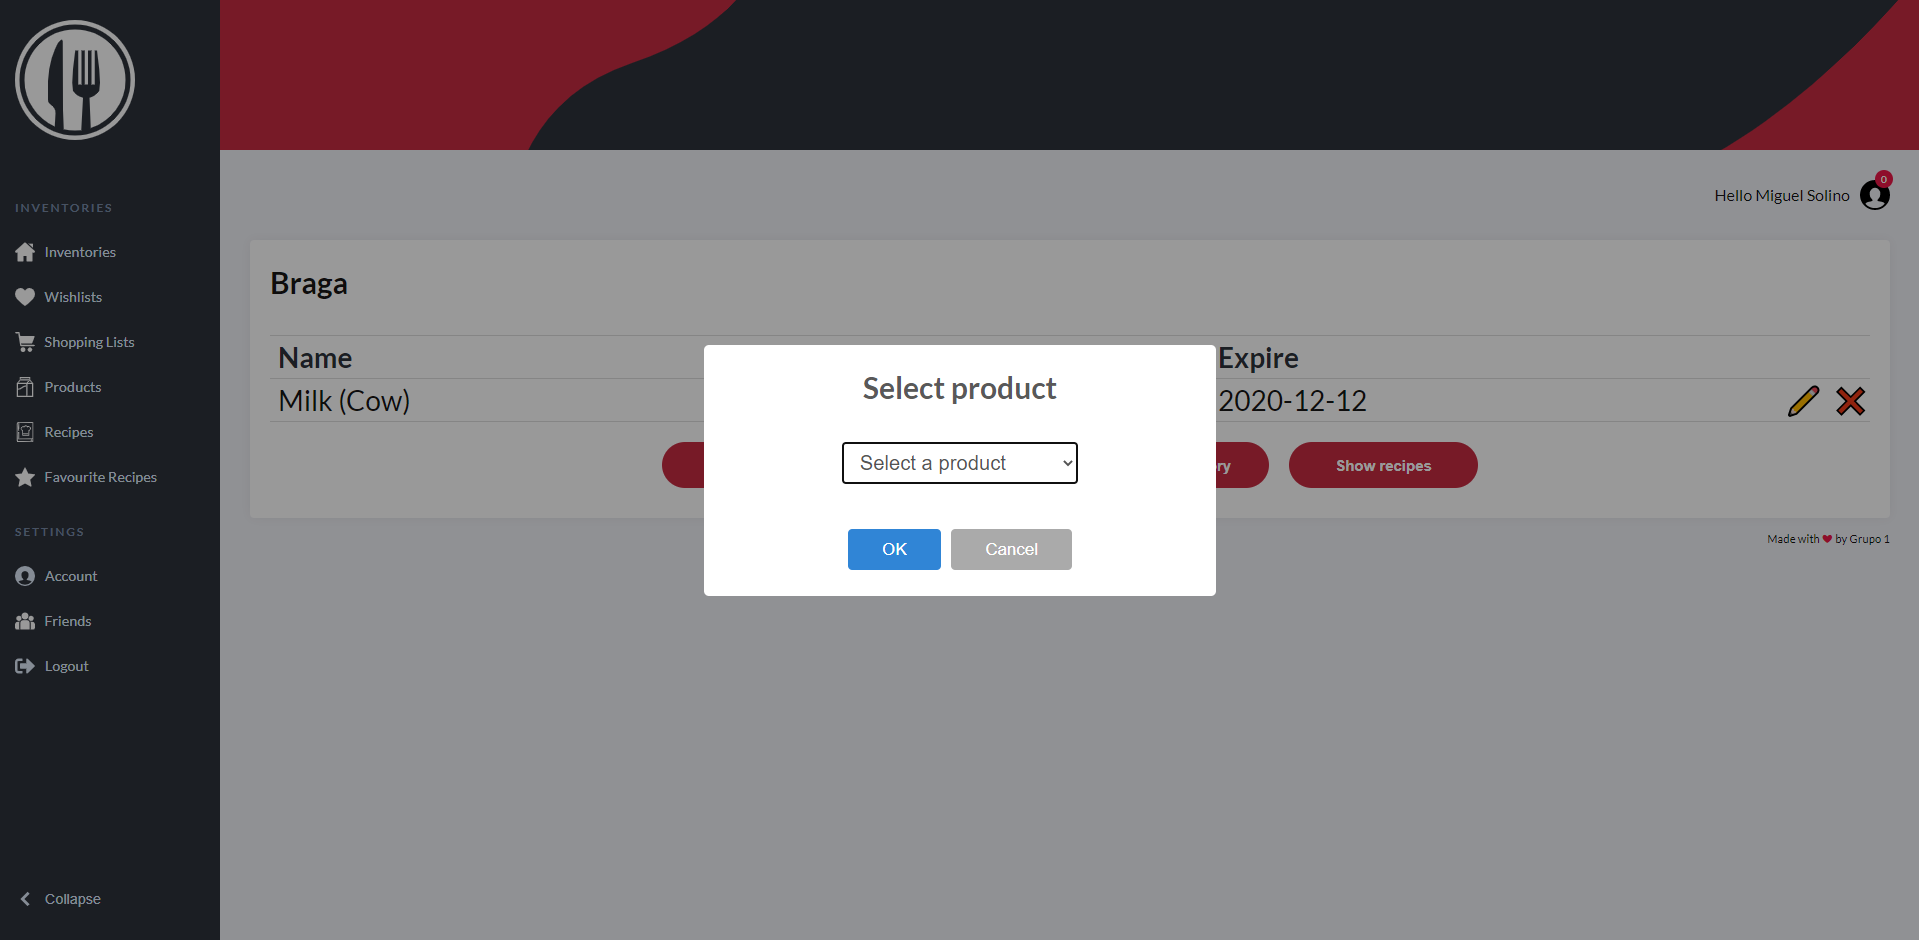
\includegraphics[width=\textwidth]{images/produto_final/inserir_produto_produto.png}
    \end{figure}

    \begin{figure}[H]
        \centering
            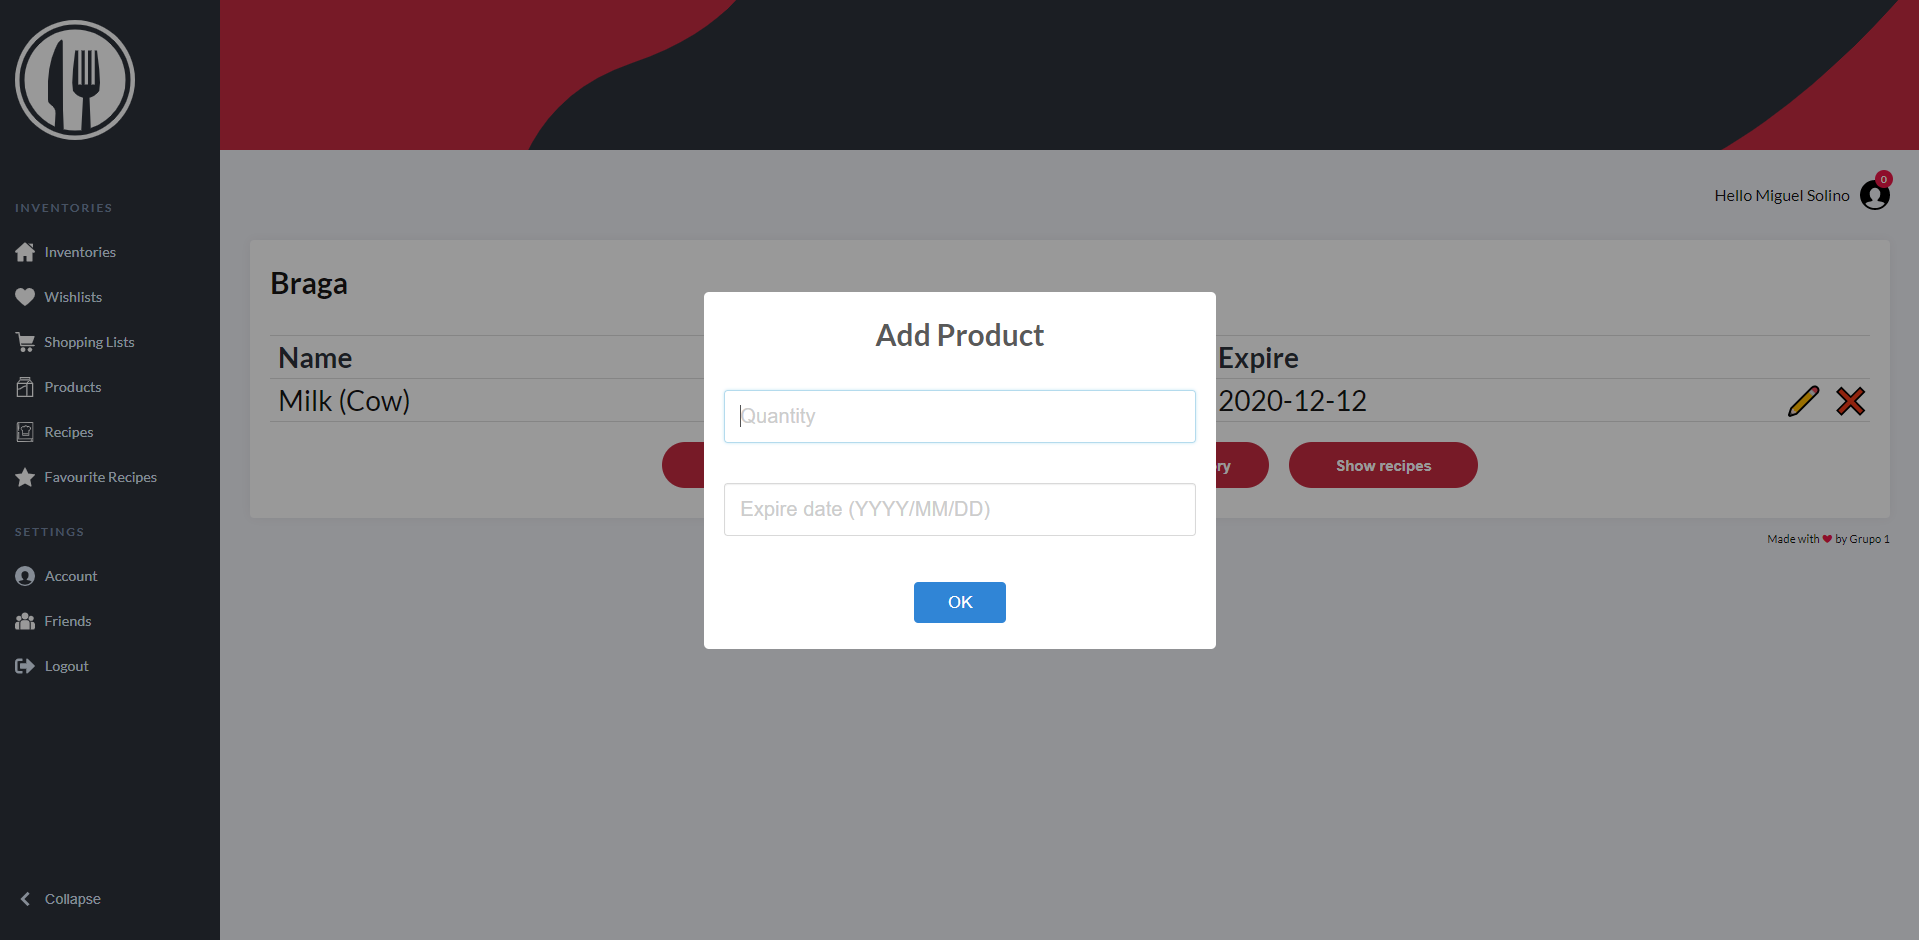
\includegraphics[width=\textwidth]{images/produto_final/inserir_produto_quantidade.png}
    \end{figure}

    \begin{figure}[H]
        \centering
            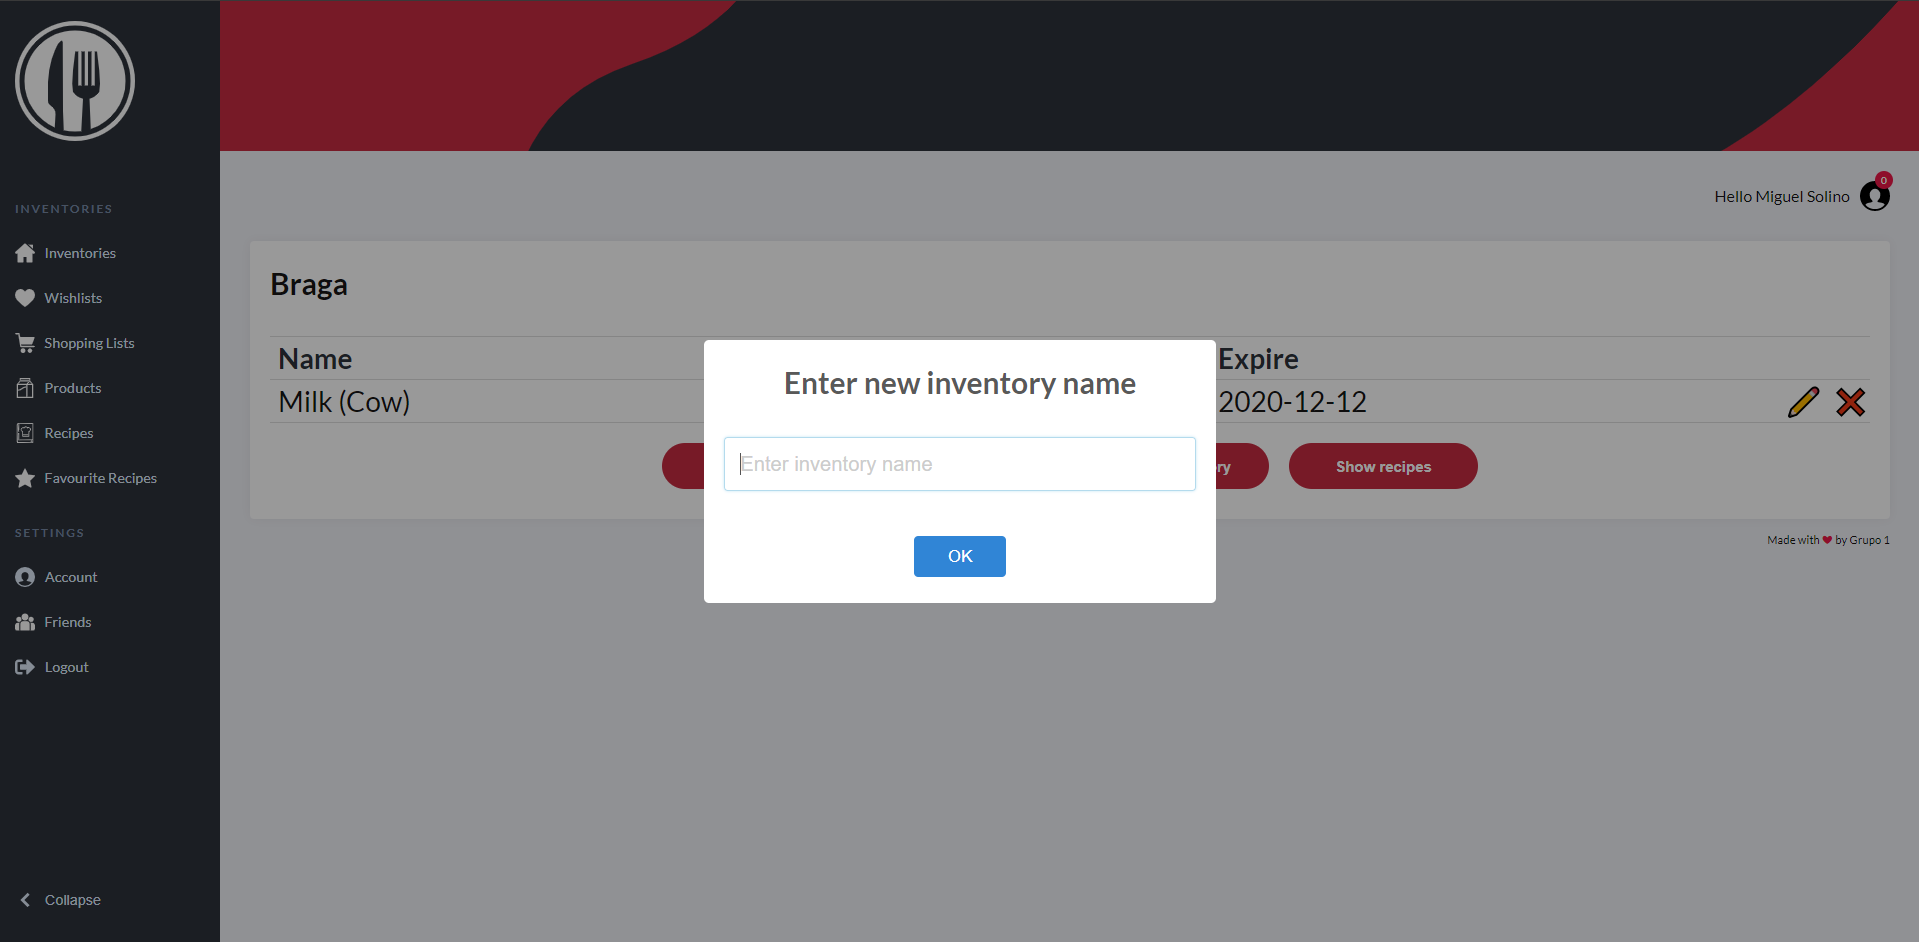
\includegraphics[width=\textwidth]{images/produto_final/alterar_nome_iventario.png}
    \end{figure}

    \begin{figure}[H]
        \centering
            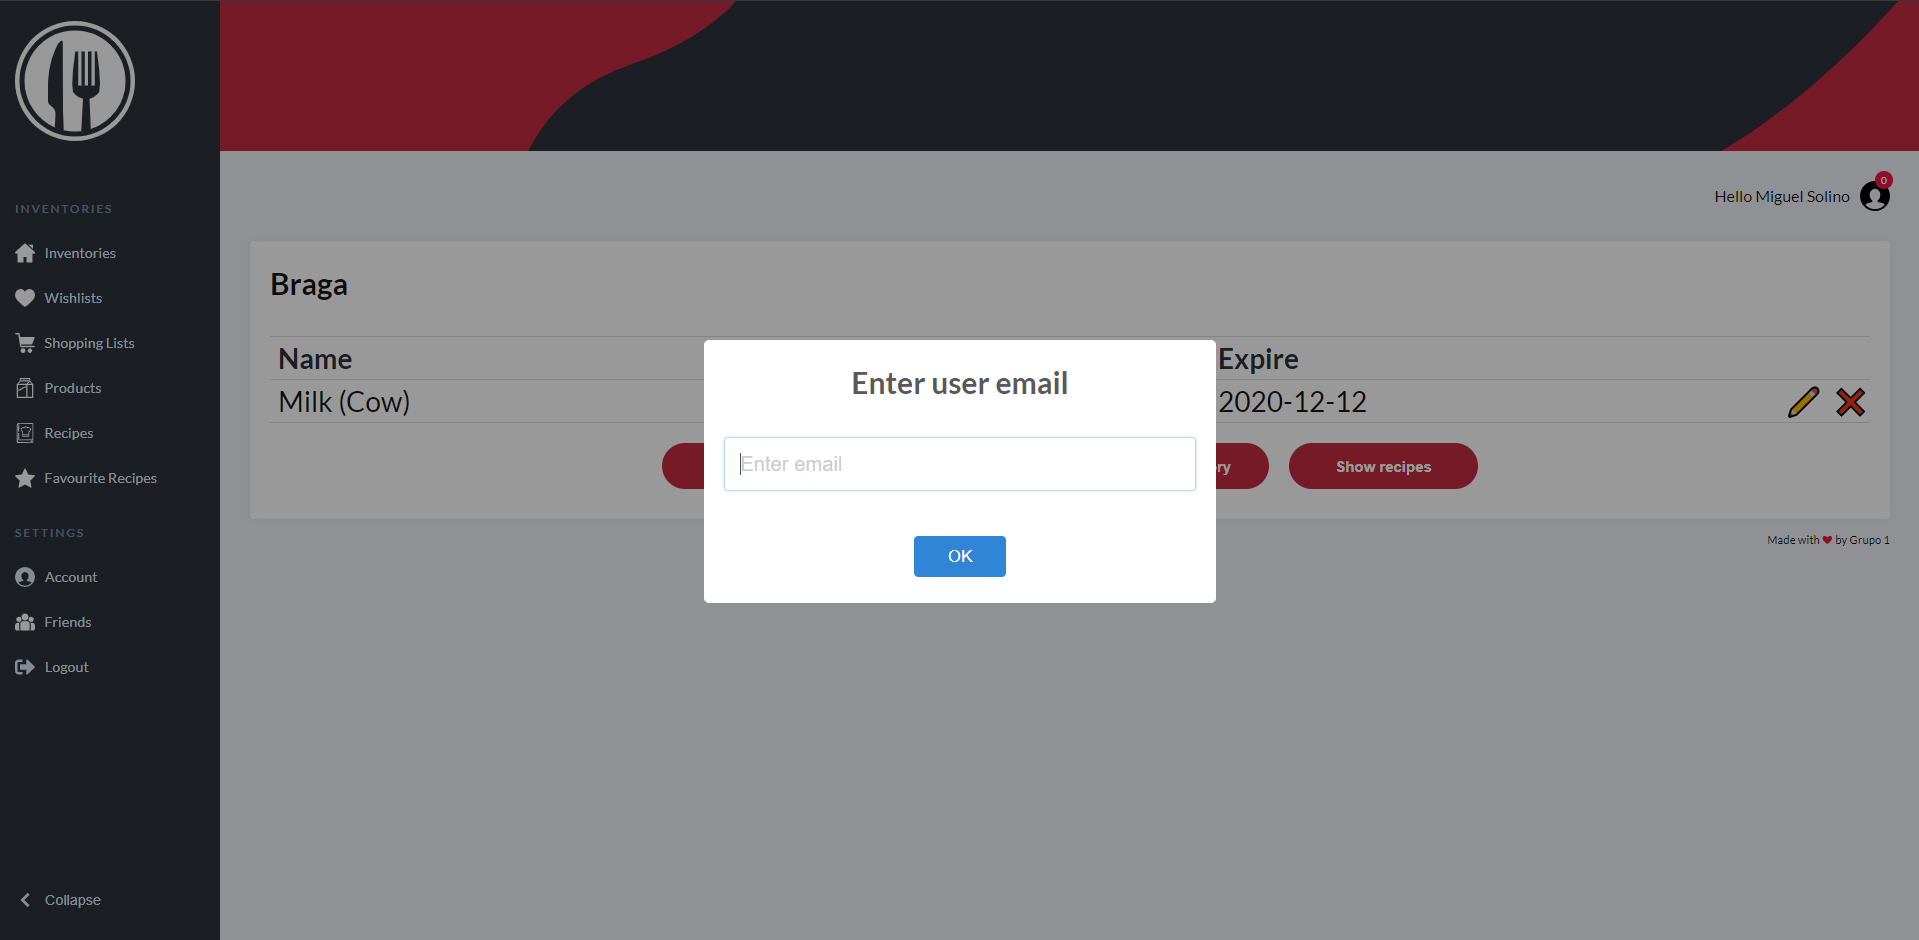
\includegraphics[width=\textwidth]{images/produto_final/partilhar_com_outro_utilizador.png}
    \end{figure}

    \begin{figure}[H]
        \centering
            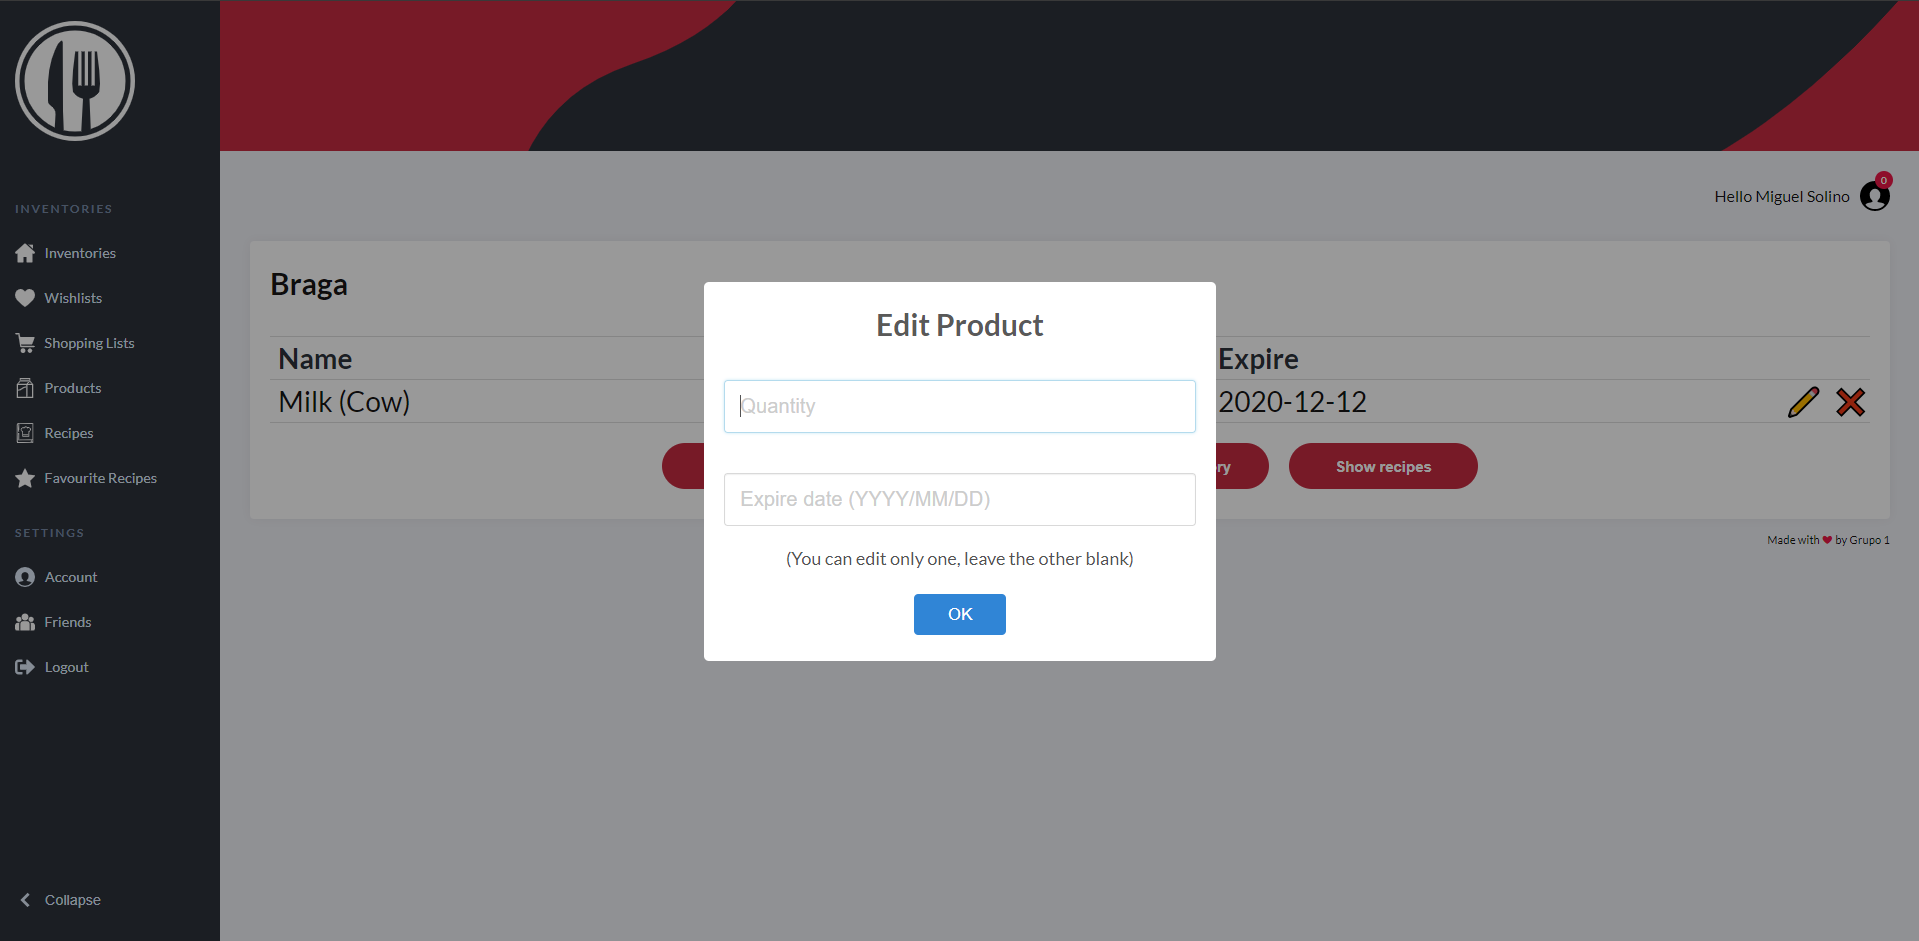
\includegraphics[width=\textwidth]{images/produto_final/editar_produto.png}
    \end{figure}

    \begin{figure}[H]
        \centering
            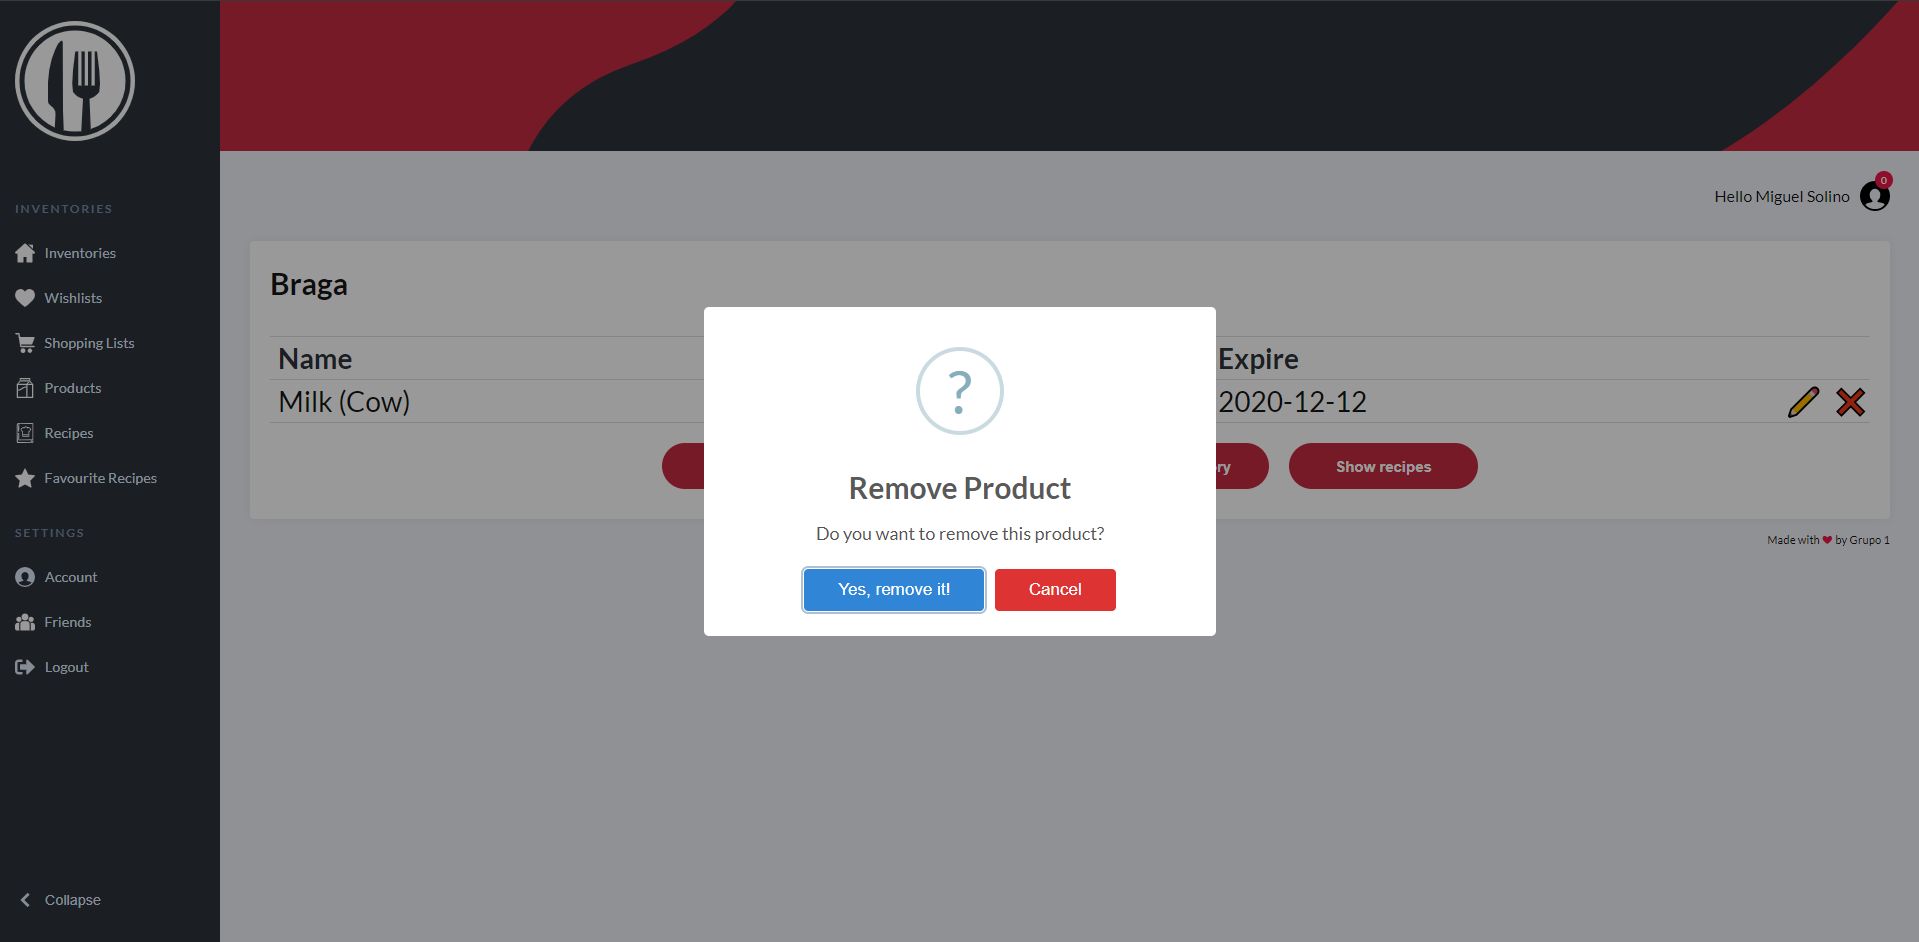
\includegraphics[width=\textwidth]{images/produto_final/eliminar_produto.png}
    \end{figure}

    \begin{figure}[H]
        \centering
            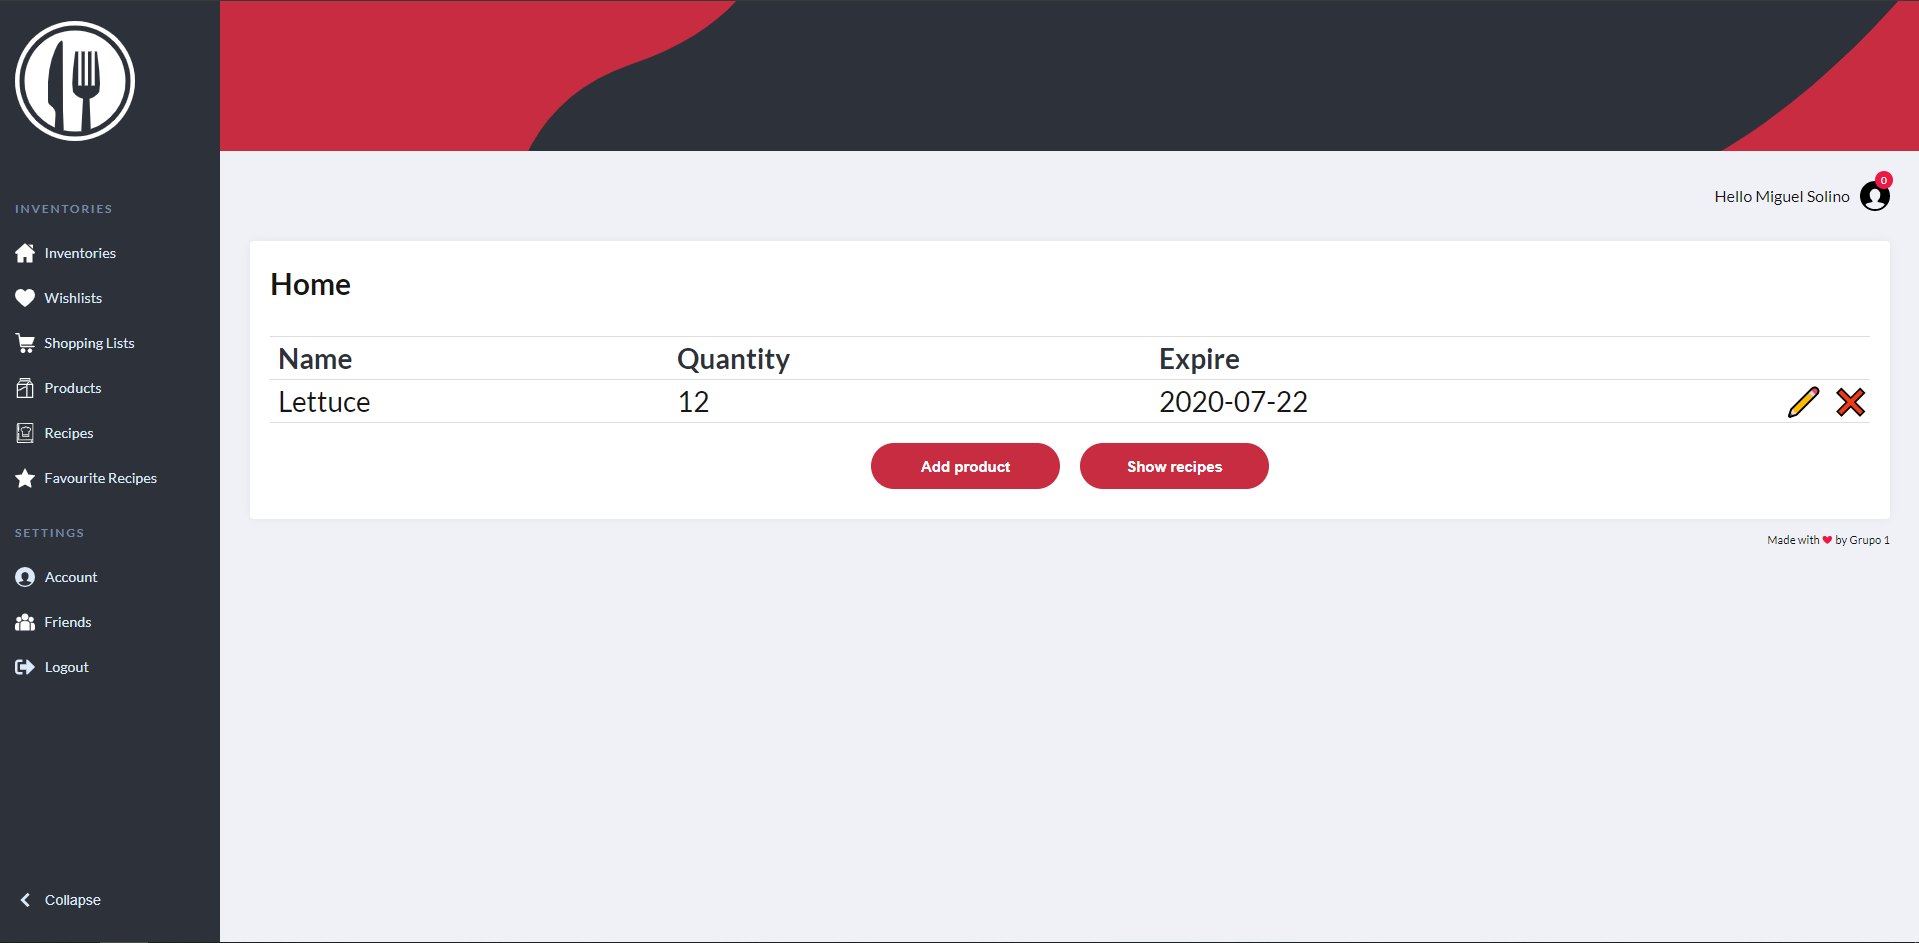
\includegraphics[width=\textwidth]{images/produto_final/pagina_iventario_partilhado.png}
    \end{figure}

    Os wishlists e as listas de compras não são apresentados aqui devido ao 
    design e as funcionalidades implementadas em cada um deles serem 
    minimamente semelhantes para não ser necessário apresentar capturas de 
    ecrã.

    \section{Produtos}

    Selecionando a opção dos \textbf{Products} do menu lateral somos
    redirecionados para esta página. Aqui é possível realizarmos uma 
    pesquisa dos produtos existentes na aplicação como também adicionar
    os mesmos a cada uma das listas existentes (despensas, wishlists e 
    listas de compras). Abaixo é apresentado o processo de como esta 
    página funciona.

    \begin{figure}[H]
        \centering
            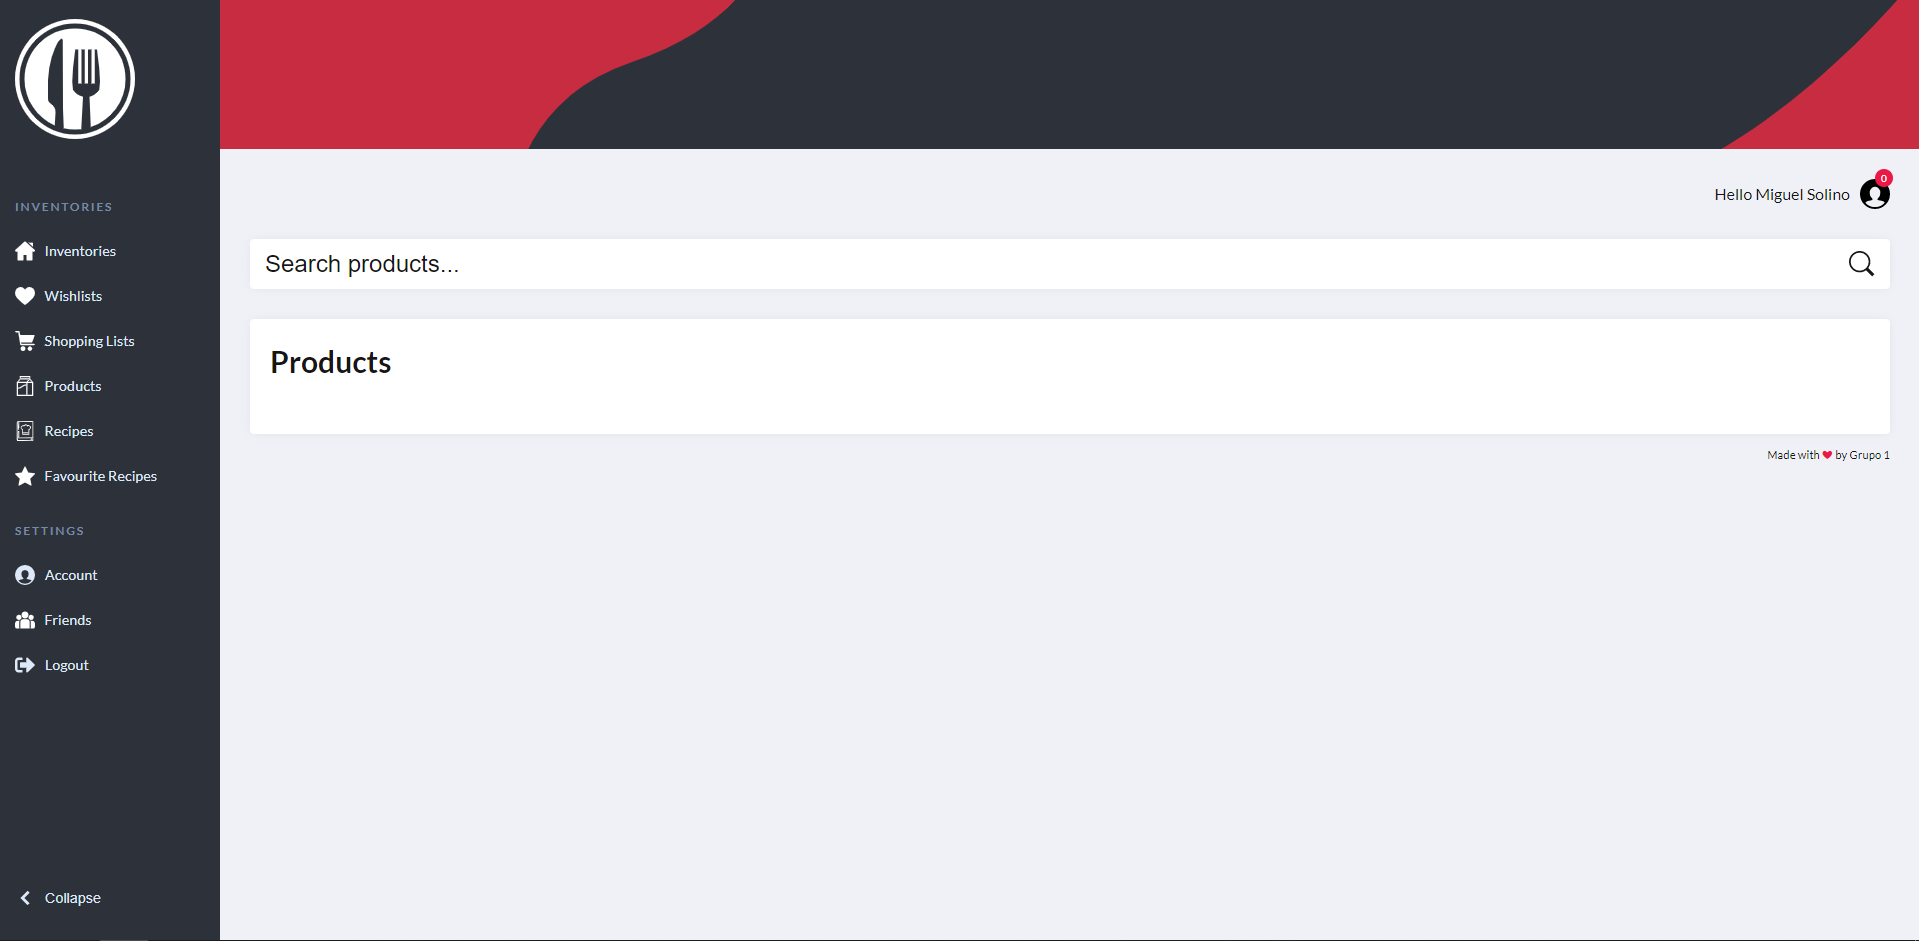
\includegraphics[width=\textwidth]{images/produto_final/procura_de_produtos.png}
    \end{figure}

    \begin{figure}[H]
        \centering
            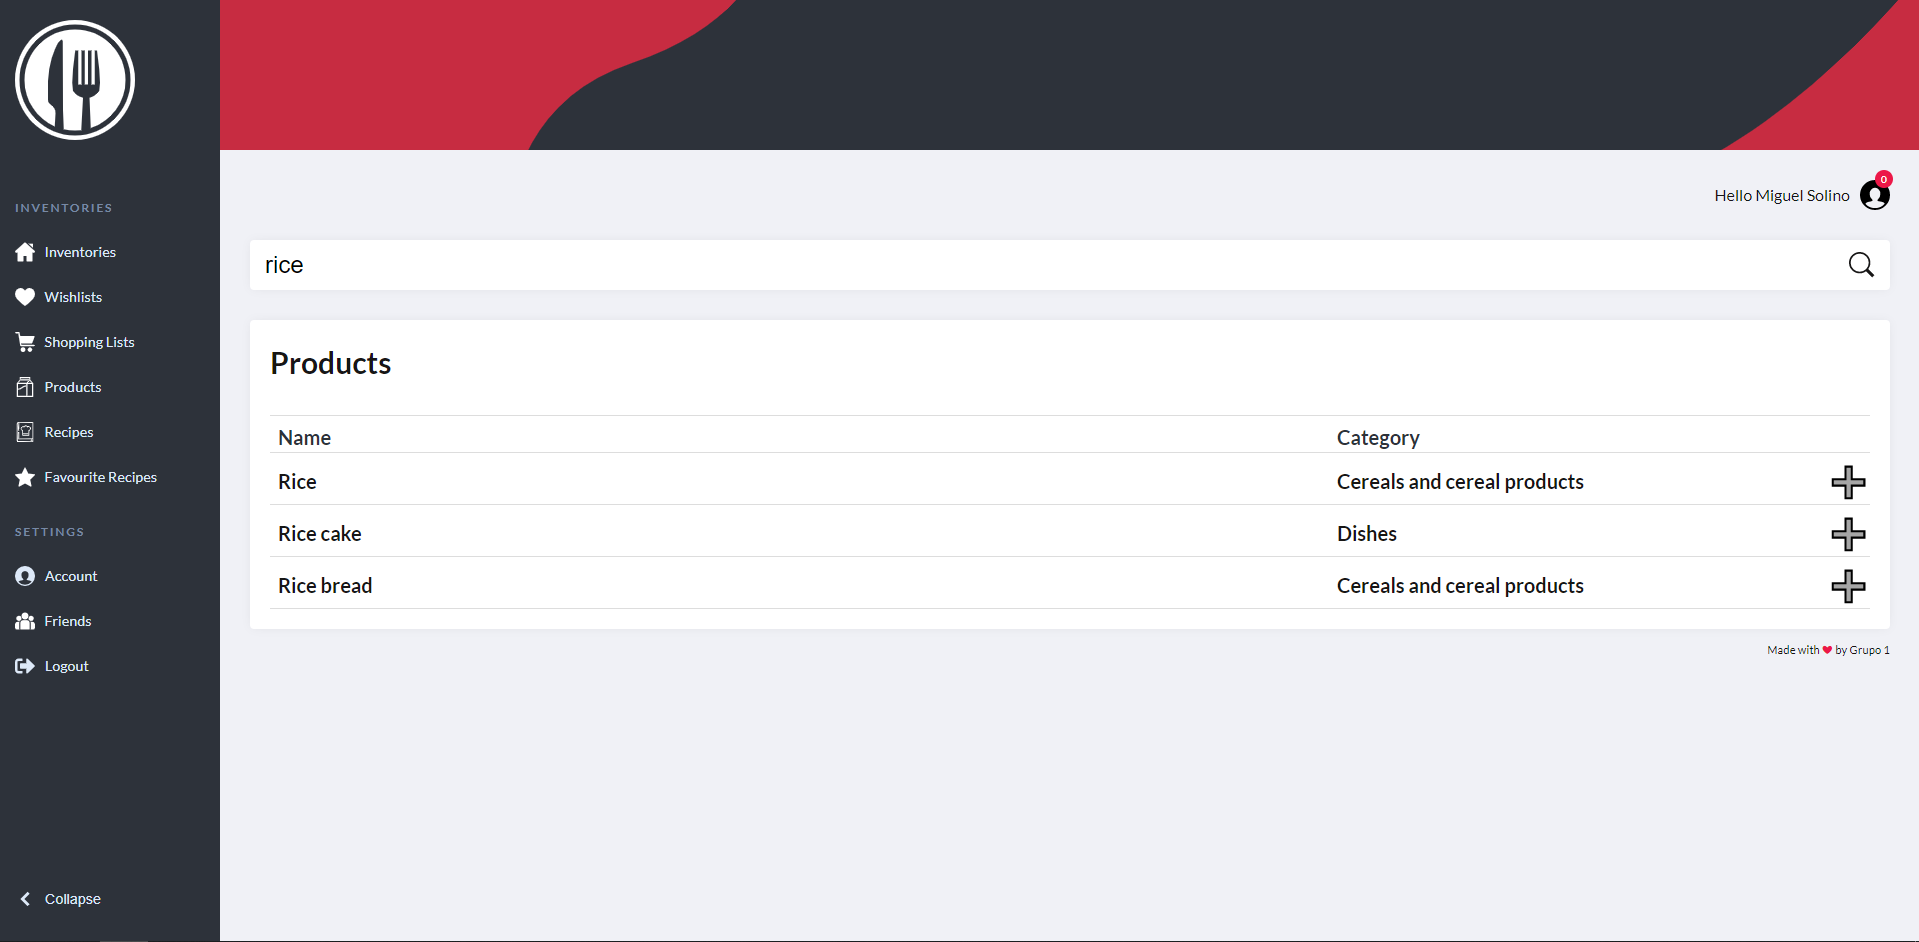
\includegraphics[width=\textwidth]{images/produto_final/procura_de_produtos_efetuada.png}
    \end{figure}

    \section{Receitas}

    Continuando agora para a opção de \textbf{Recipes} no menu lateral a 
    aplicação redireciona o utilizador para a página abaixo onde poderá,
    semelhante à página de procura de receitas, realizar uma pesquisa
    das receitas existentes na aplicação e escolher as que mais gostar
    como favoritas para mais tarde serem apresentadas e consultadas na
    página de receitas favoritas do utilizador.

    \begin{figure}[H]
        \centering
            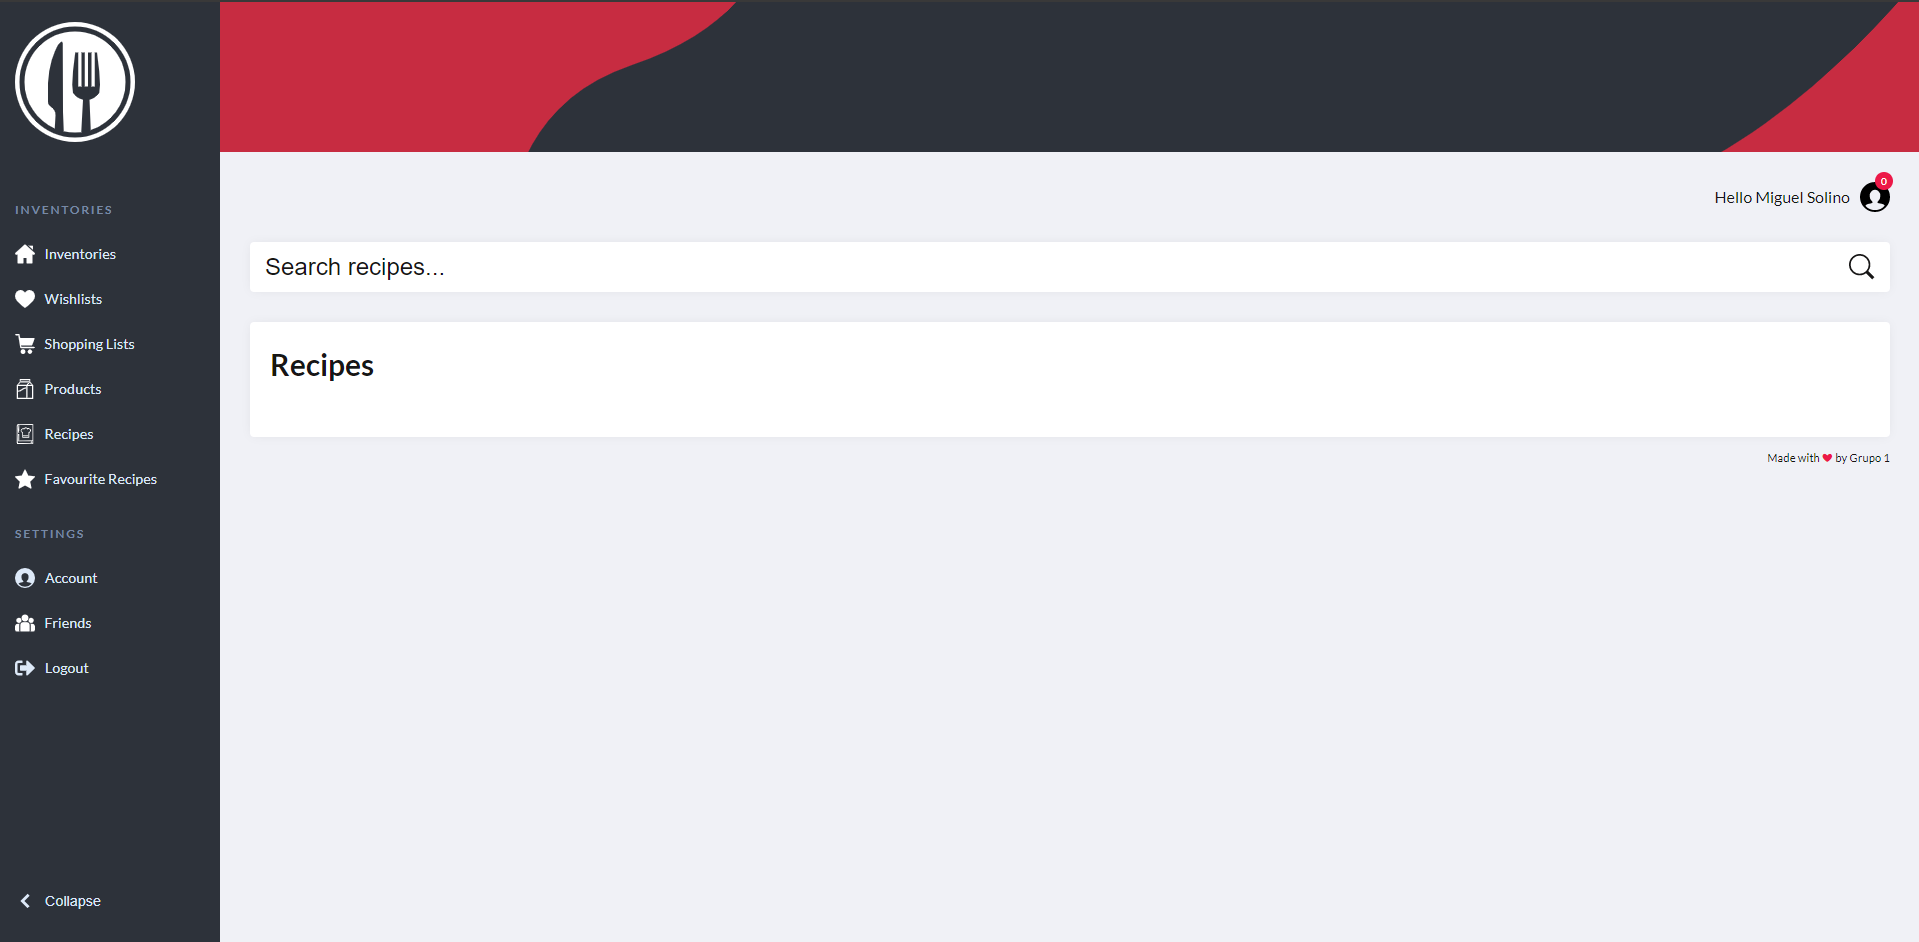
\includegraphics[width=\textwidth]{images/produto_final/procura_de_receitas.png}
    \end{figure}

    \begin{figure}[H]
        \centering
            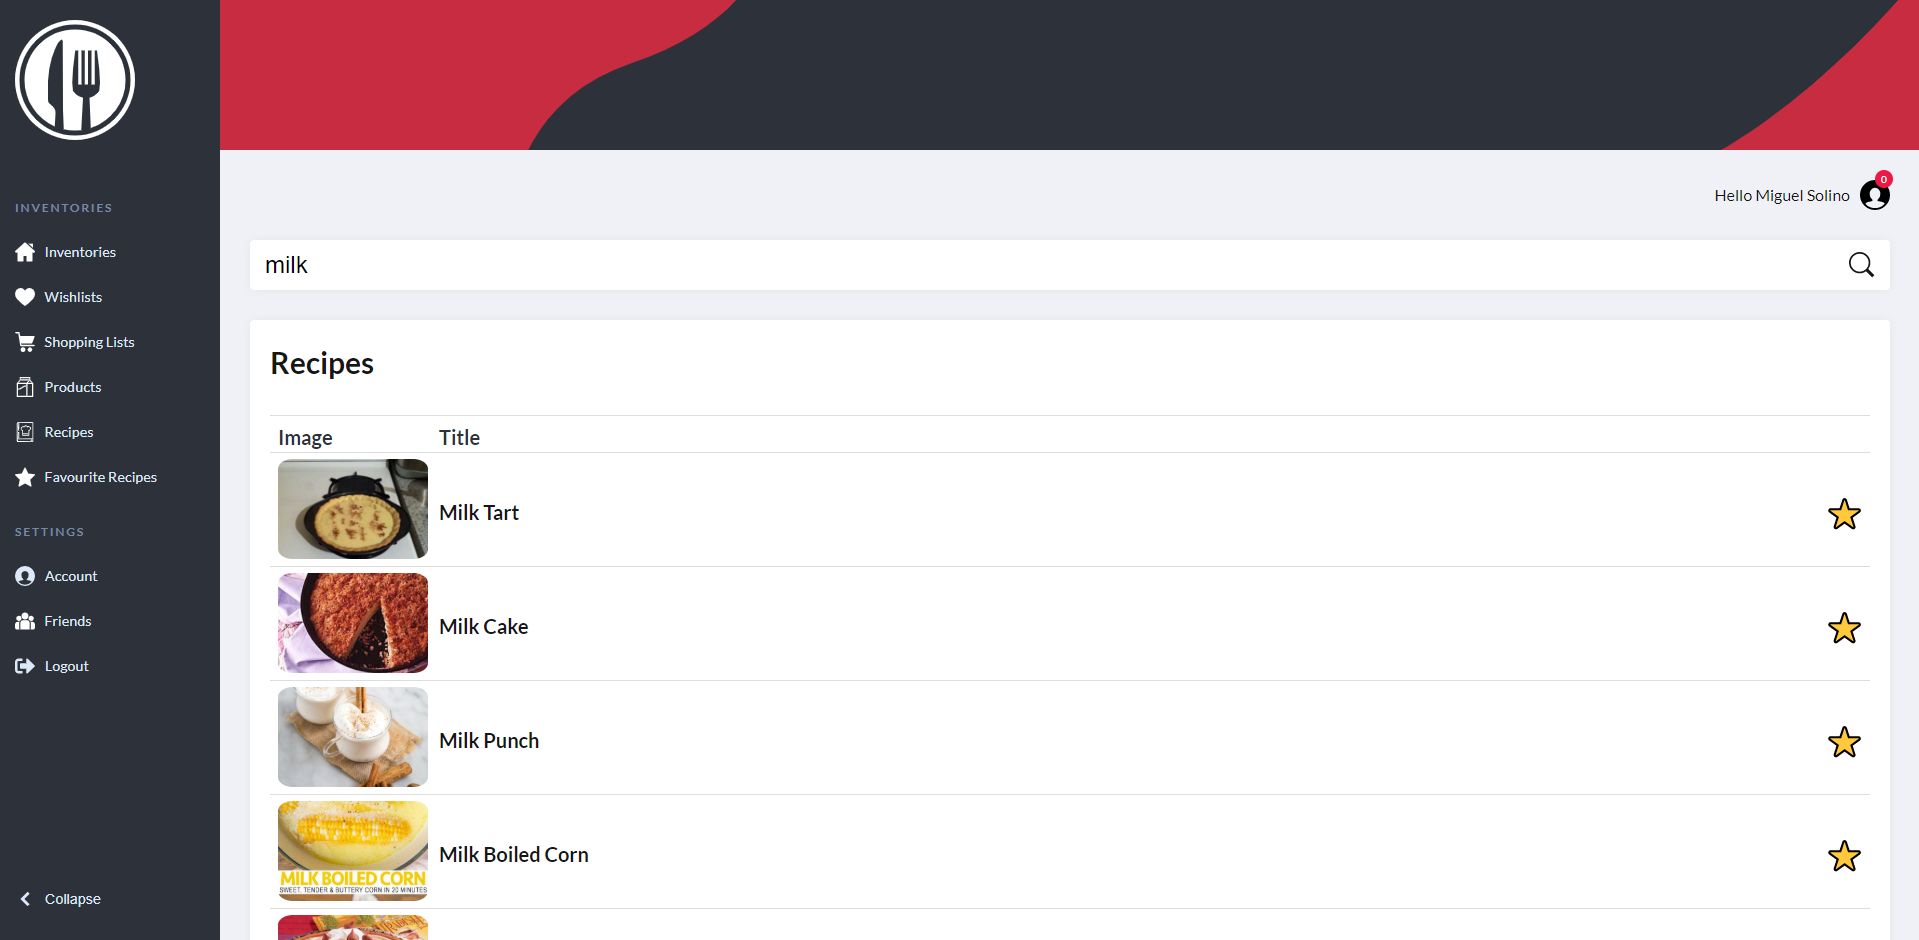
\includegraphics[width=\textwidth]{images/produto_final/procura_de_receitas_efetuadas.png}
    \end{figure}

    Selecionando uma receita da lista será possível ver os detalhes da
    da mesma (imagem, sumário, ingredientes e isntruções), como na 
    figura abaixo.

    \begin{figure}[H]
        \centering
            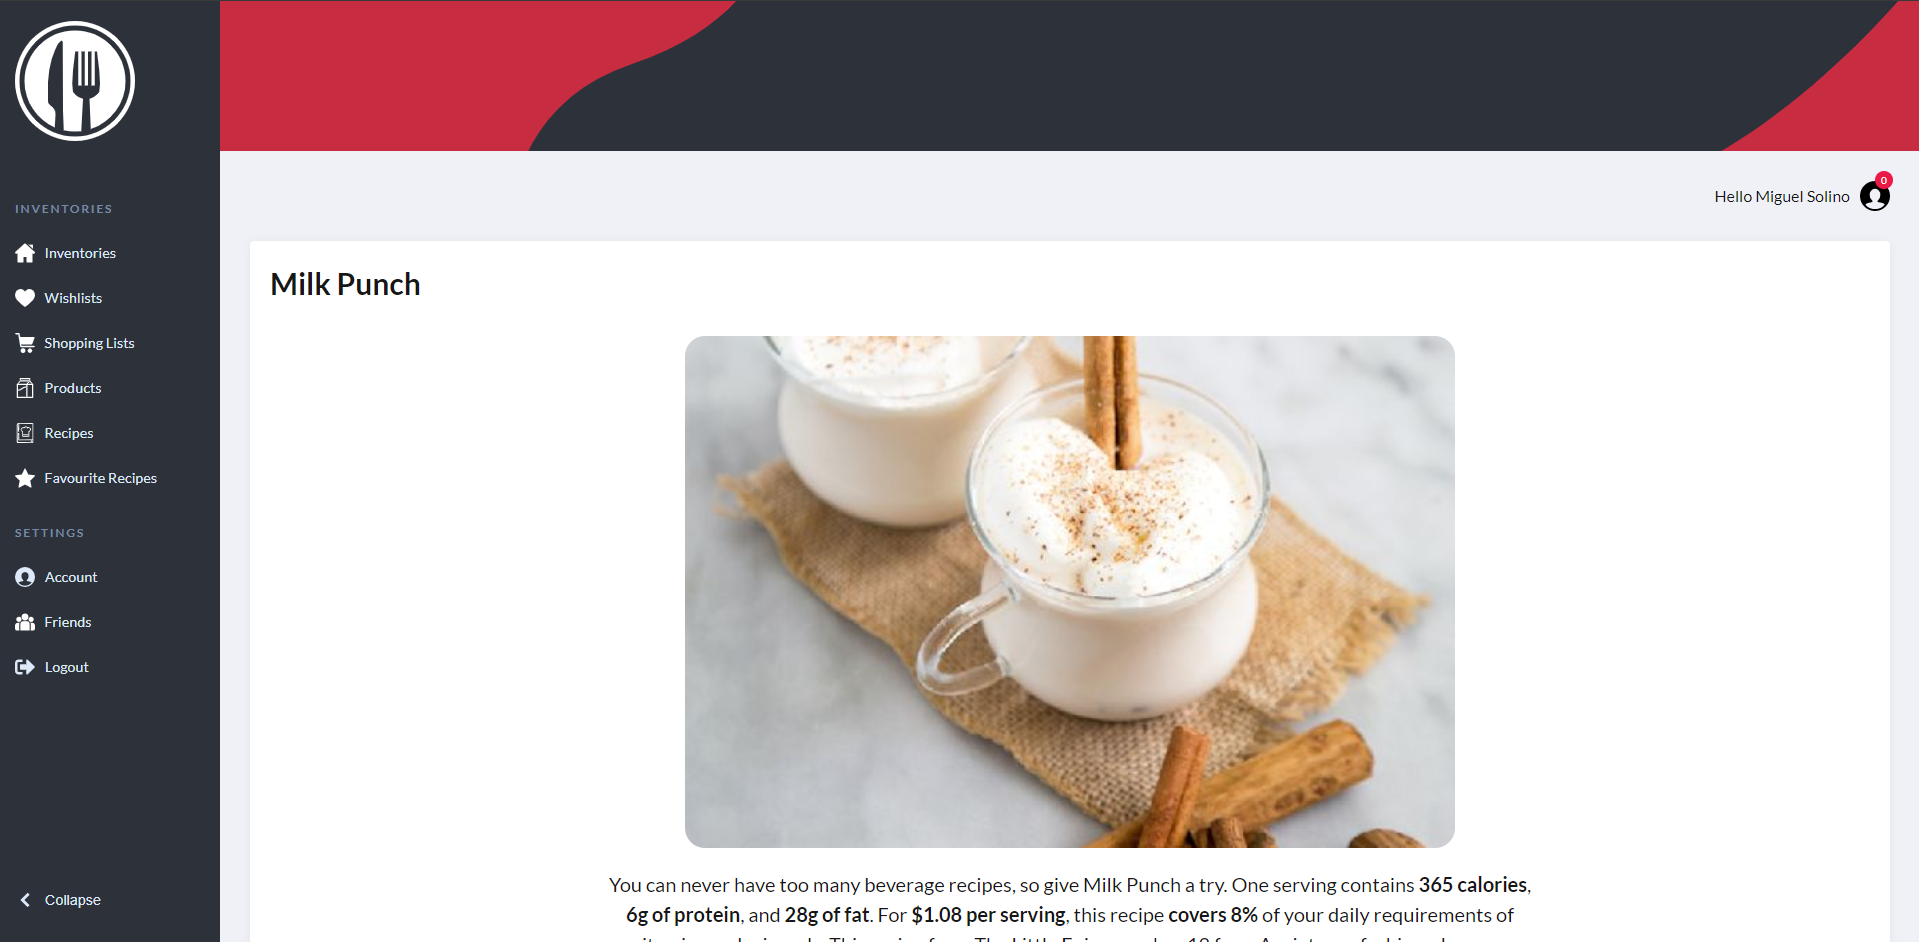
\includegraphics[width=\textwidth]{images/produto_final/receitas.png}
    \end{figure}

    \section{Receitas favoritas}
    Na secção anterior foi feita uma referência à pagina de receitas favoritas
    de um utilizador. Esta é acessível a partir da opção 
    \textbf{Favourite Recipes} do menu lateral e a página apresentada ao 
    utilizador é a figura abaixo. Aqui será possivel serem consultadas as
    receitas que o utilizador colocou como favoritas e remove-las.

    \begin{figure}[H]
        \centering
            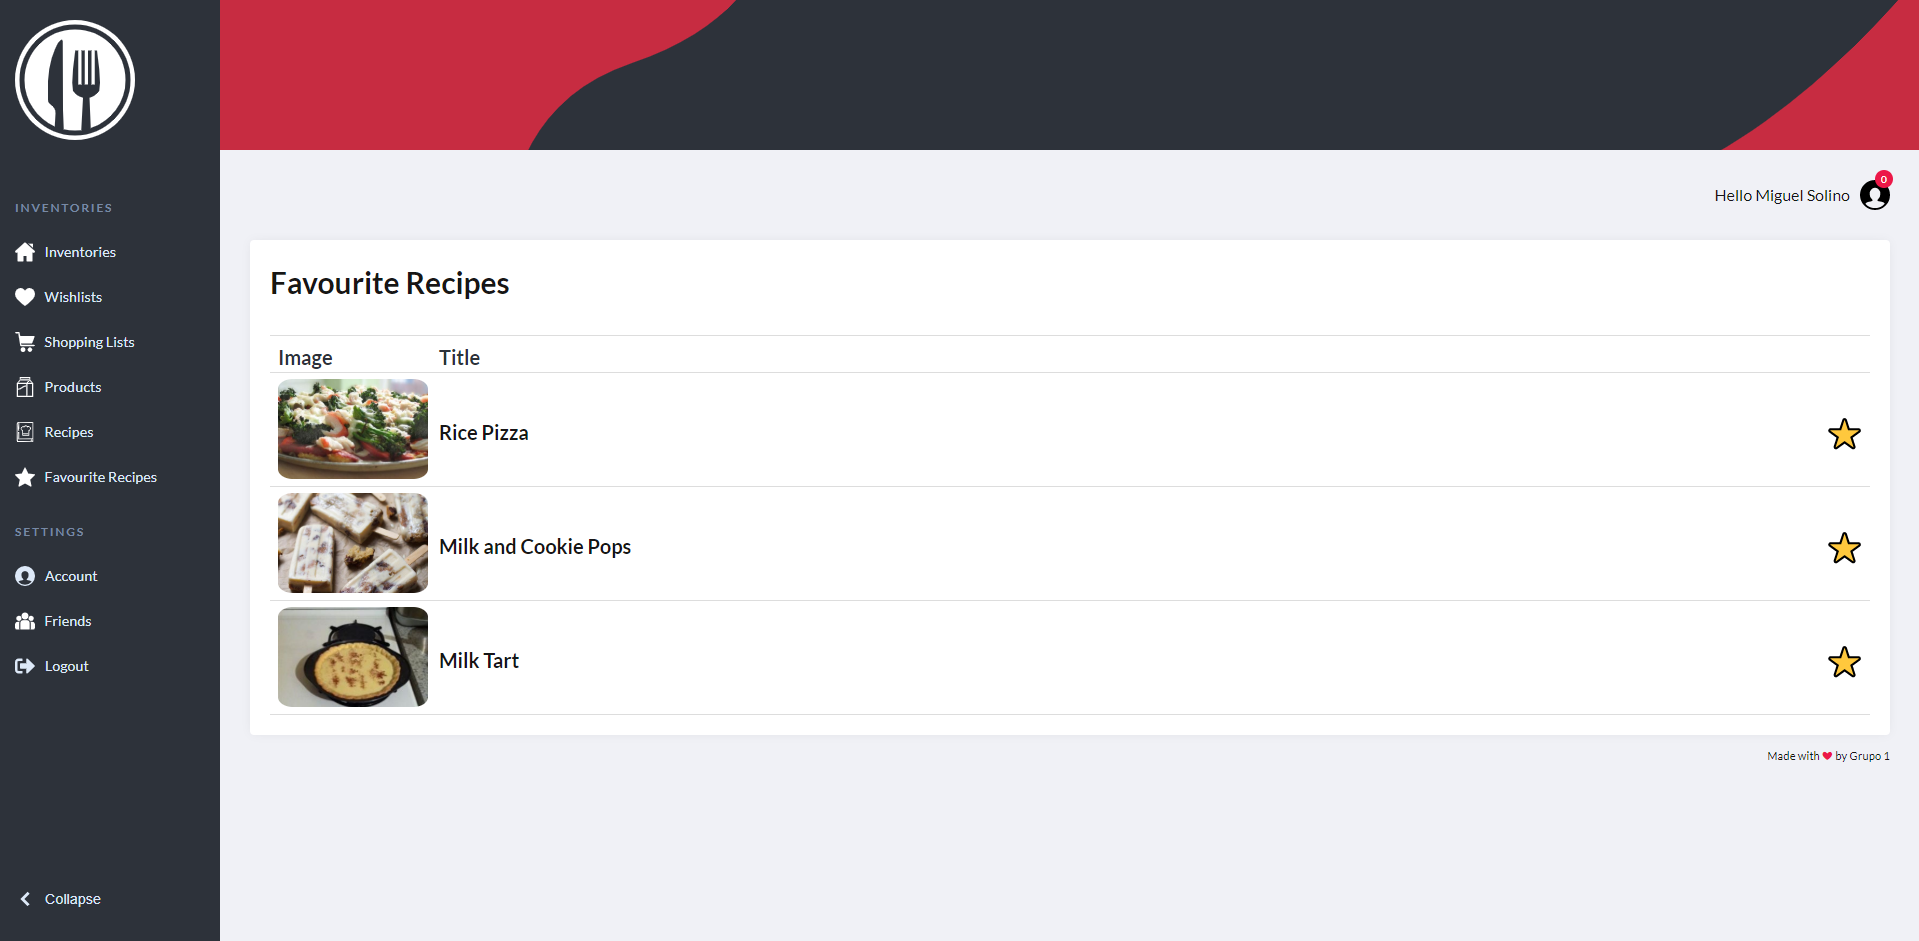
\includegraphics[width=\textwidth]{images/produto_final/receitas_favoritas.png}
    \end{figure}

    \section{Perfil}

    Passando à secção de \textbf{Settings} do menu lateral, e começando pelo 
    \textbf{Account}, é apresentado ao utilizador os seus dados, nomeadamente,
    nome, email, número de telemóvel e data de nascimento. Todos estes dados, 
    exceto o de email, são editáveis caso o utilizador os pretenda mudar.

    \begin{figure}[H]
        \centering
            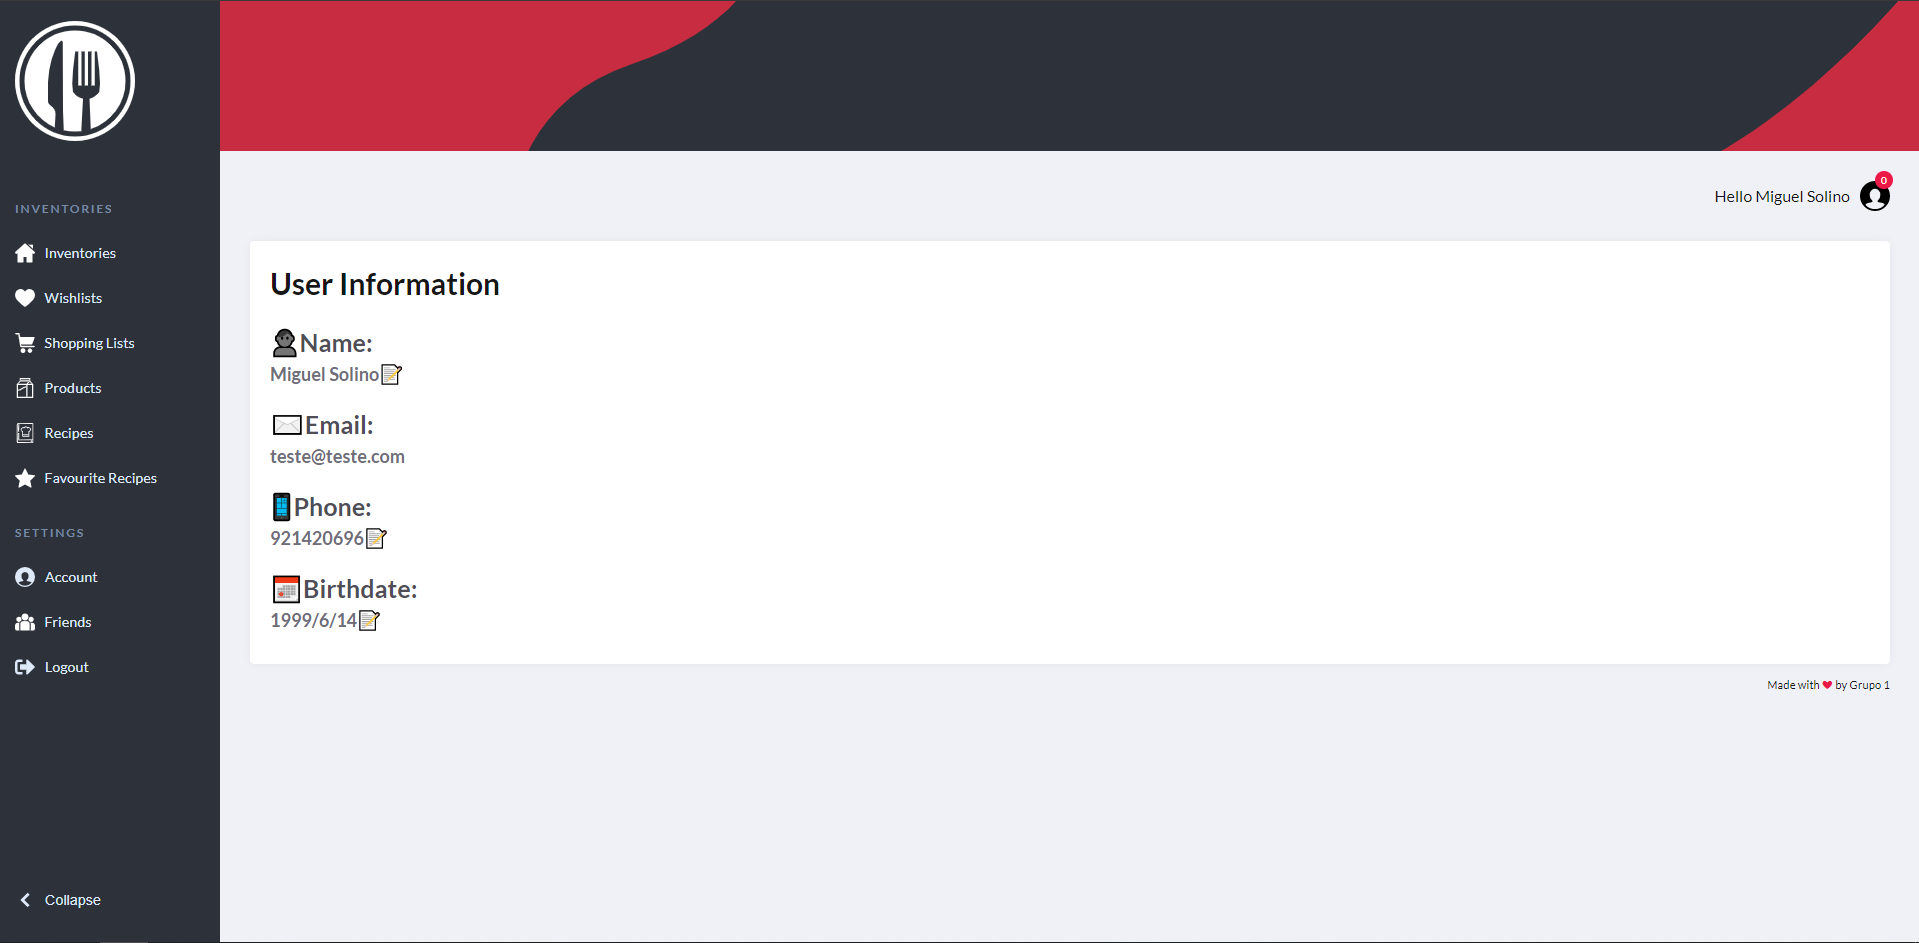
\includegraphics[width=\textwidth]{images/produto_final/pagina_de_perfil.png}
    \end{figure}

    \begin{figure}[H]
        \centering
            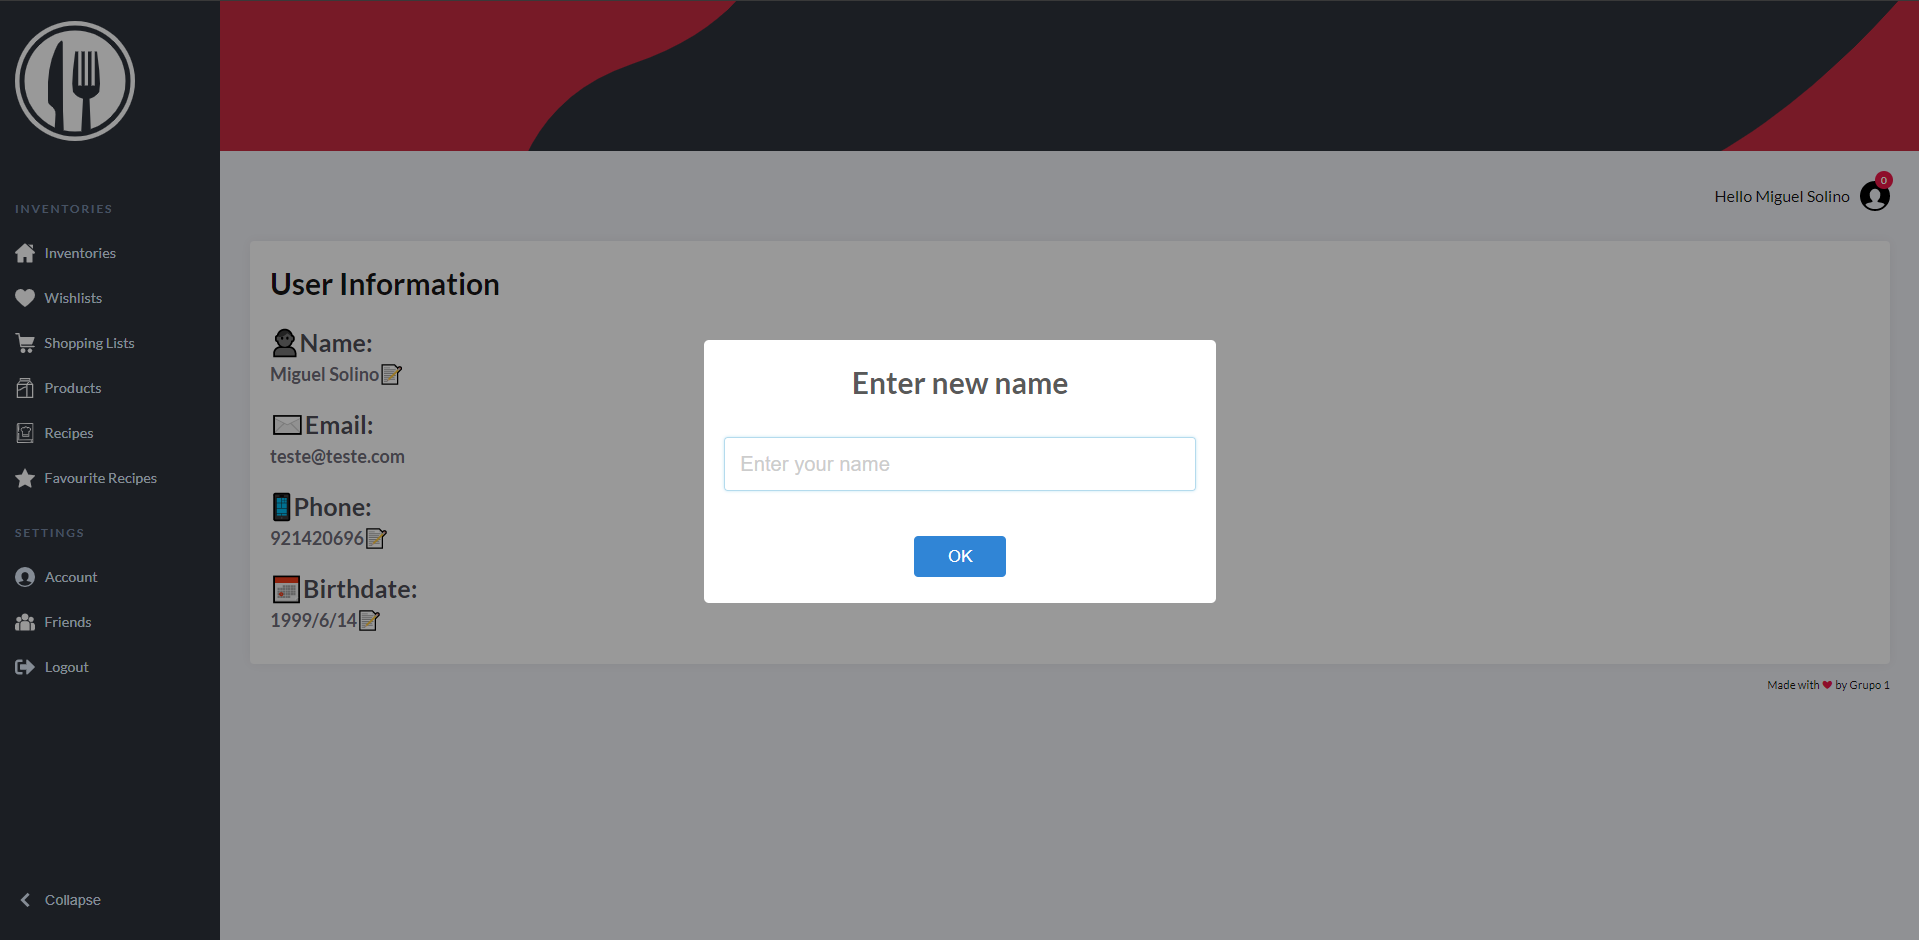
\includegraphics[width=\textwidth]{images/produto_final/alterar_nome_perfil.png}
    \end{figure}

    \begin{figure}[H]
        \centering
            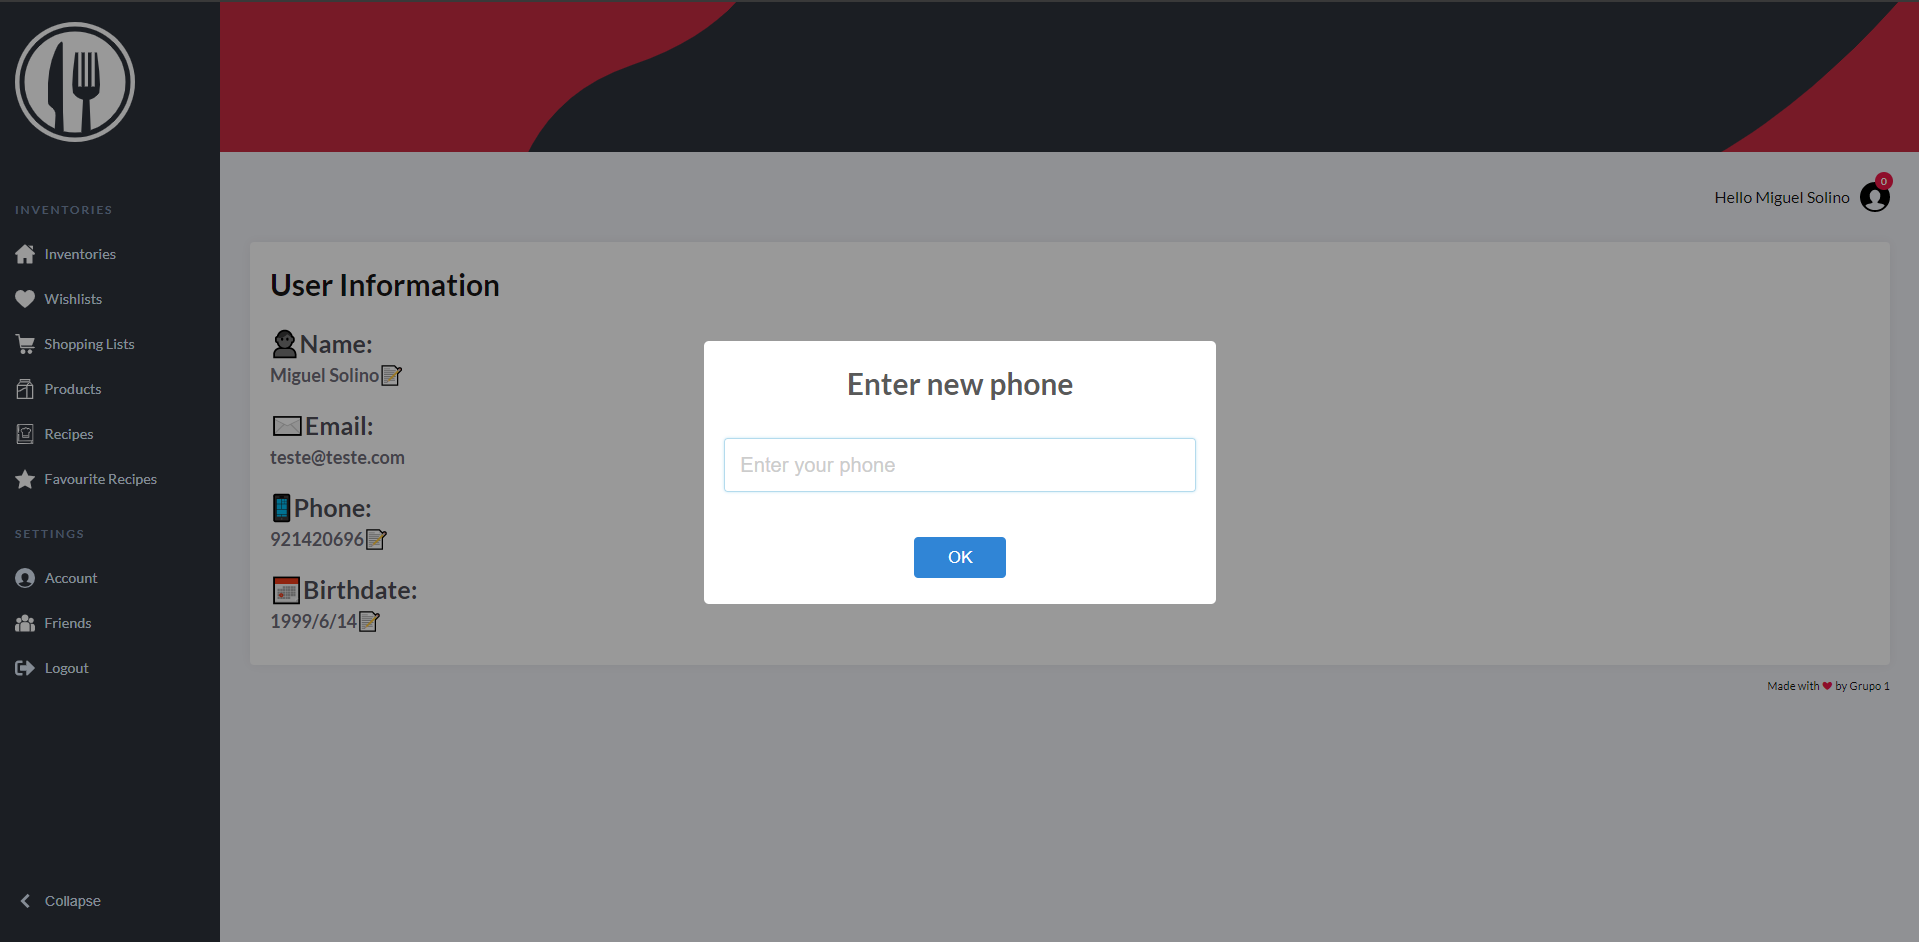
\includegraphics[width=\textwidth]{images/produto_final/alterar_numero_perfil.png}
    \end{figure}

    \begin{figure}[H]
        \centering
            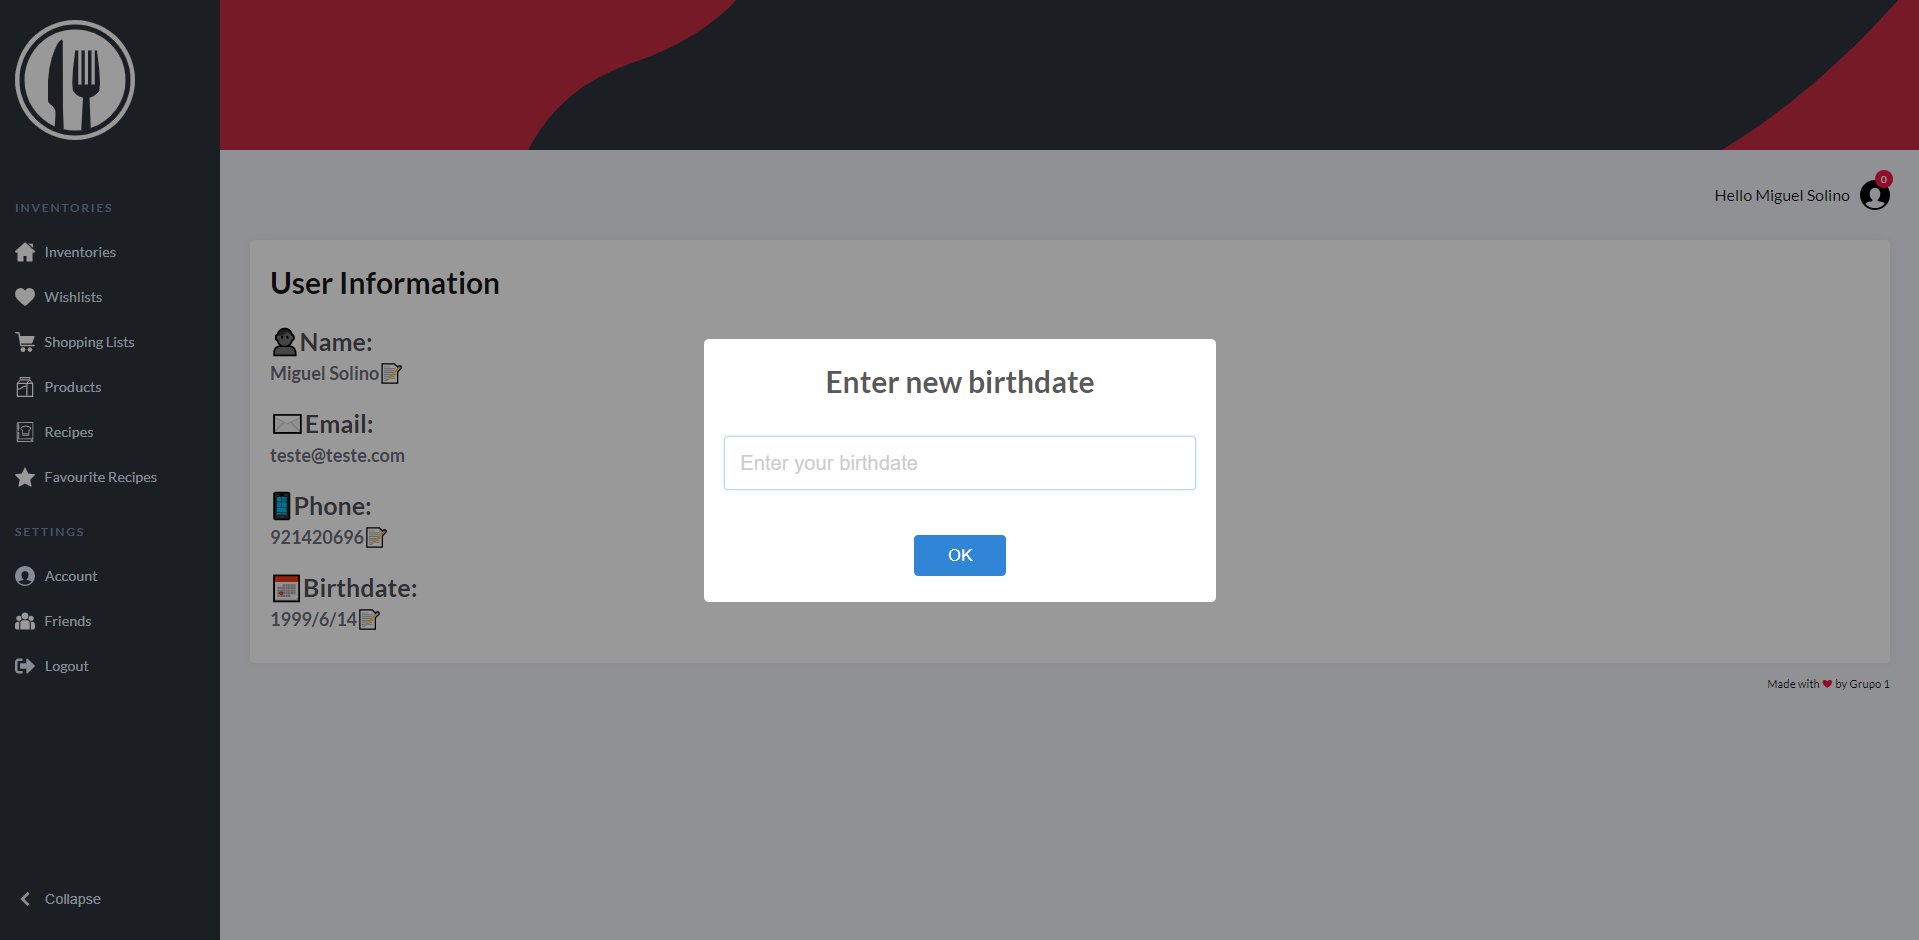
\includegraphics[width=\textwidth]{images/produto_final/alterar_nascimento_iventario.png}
    \end{figure}

    \section{Amigos}

    Na segunda opção da mesma secção, \textbf{Friends}, temos presente o botão
    que redireciona o utilizador para a sua página de amigos. Aqui é onde 
    se poderá adicionar e remover amigos e responder a pedidos de amizade
    recebidos. 

    \begin{figure}[H]
        \centering
            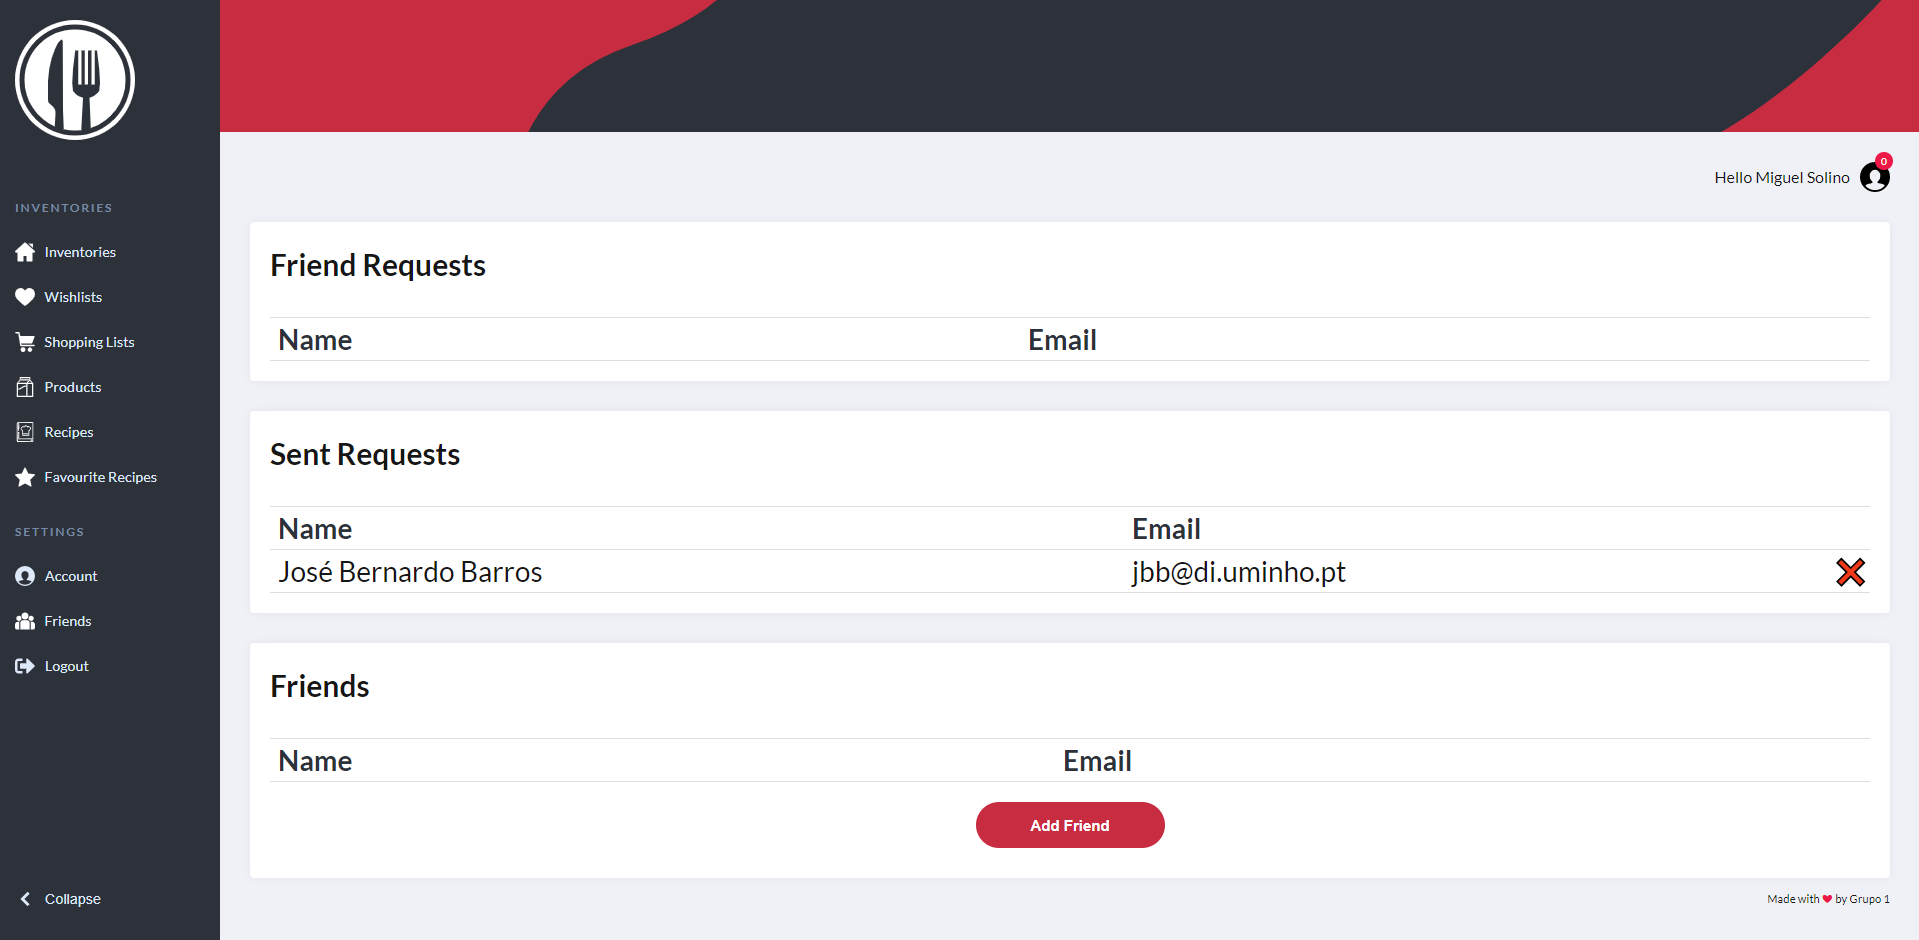
\includegraphics[width=\textwidth]{images/produto_final/pedido_amigos_enviado.png}
    \end{figure}

    \begin{figure}[H]
        \centering
            \includegraphics[width=\textwidth]{images/produto_final/adicionar_amigo.png}
    \end{figure}

    \begin{figure}[H]
        \centering
            \includegraphics[width=\textwidth]{images/produto_final/pedido_recebido.png}
    \end{figure}

    \begin{figure}[H]
        \centering
            \includegraphics[width=\textwidth]{images/produto_final/amigo_adicionado.png}
    \end{figure}

    \section{Popup Erro/Sucesso}

    Abaixo são apresentados exemplos de como são os popups de \textbf{Sucesso} 
    e \textbf{Erro} para as diferentes funcionalidades da aplicação.

    \begin{figure}[H]
        \centering
            \includegraphics[width=\textwidth]{images/produto_final/exemplo_erro.png}
    \end{figure}

    \begin{figure}[H]
        \centering
            \includegraphics[width=\textwidth]{images/produto_final/exemplo_sucesso.png}
    \end{figure}

    \section{Painel de Notificações}

    Finalmente, abaixo está o nosso painel de notificações que apresentará
    notificações quando o utilizador tiver pedidos de amizade por aceitar
    ou produtos dos inventários perto de ficarem fora de validade ou 
    já expirados.

    \begin{figure}[H]
        \centering
            \includegraphics[width=\textwidth]{images/produto_final/notificacoes.png}
    \end{figure}

\chapter{Conclusões}
    Conluindo, atingimos todos os objetivos propostos cumprindo todas as tarefas
    propostas entre cada \textit{sprint} e cumprir o calendário estipulado
    inicialmente no diagrama de Gantt.\\
    Para além do melhor domínio das novas tecnologias utilizadas na produção
    deste \textit{software} também ganhamos um melhor domínio sobre metodologias
    de desenvolvimento e organização de tarefas em equipa.\\
    Como trabalho futuro gostaríamos de desenvolver uma aplicação mobile
    facilitando a utilização do produto e assim expandir o público alvo.
    Gostaríamos também de trabalhar melhor a integração com a API externa \textit{spoonacular}.

\end{document}

